%% \documentclass[handout,t]{beamer} % HANDOUT
%% \documentclass[handout,notes=show,t]{beamer} % NOTES
\documentclass[t]{beamer} % SLIDES
\usepackage{etex}

\usetheme{DSM}
\usepackage{beamer-tools-dsm}

%%
%% some useful macros: mathematical notation etc.
%%

%% abbreviations for logic symbols
\renewcommand{\implies}{\Rightarrow}
\newcommand{\equivalent}{\Leftrightarrow}

%% abbreviations for common number spaces
\newcommand{\setN}[1][]{\mathbb{N}_{#1}} % allows \setN and \setN[0]
\newcommand{\setZ}{\mathbb{Z}}
\newcommand{\setQ}{\mathbb{Q}}
\newcommand{\setR}{\mathbb{R}}

%% sets and (sub-)sets defined by condition
\newcommand{\set}[1]{\{#1\}}
\newcommand{\setdef}[2]{\set{#1\,|\,#2}}
\newcommand{\bigset}[1]{\bigl\{#1\bigr\}}
\newcommand{\bigsetdef}[2]{\bigset{#1\bigm|#2}}
\newcommand{\setscale}[1]{\left\{#1\right\}}
\newcommand{\setdefscale}[2]{\setscale{#1\left|\,#2\right.}}

%% absolute value and norm
\newcommand{\abs}[1]{\lvert #1\rvert}
\newcommand{\bigabs}[1]{\bigl\lvert #1\bigr\rvert}
\newcommand{\absscale}[1]{\left\lvert #1\right\rvert}
\newcommand{\norm}[2][]{\lVert #2\rVert_{#1}}
\newcommand{\bignorm}[2][]{\bigl\lVert #2\bigr\rVert_{#1}}
\newcommand{\normscale}[2][]{\left\lVert #2\right\rVert_{#1}}

%% complement set (with optional index)
\newcommand{\compl}[1][]{\mathcal{C}^{#1}}

%% power set: \powerset{\Sigma^*}
\newcommand{\powerset}[1]{\mathcal{P}(#1)}

%% uparrow: a \ua b = direct dominance in ordered tree
\newcommand{\ua}{\uparrow}

%% left-right arrow: this $\lra$ that
\newcommand{\lra}{\leftrightarrow}

%% expanded engineering notation: 4.2\x\e+5
\newcommand{\e}[2]{10^{\ifthenelse{\equal{#1}{+}}{}{#1}#2}}
\newcommand{\x}{\cdot}

%% arg max & min: \argmax_{x\in C}, \argmin_{x\in C}
\newcommand{\argmax}{\mathop{\text{arg~max}}}
\newcommand{\argmin}{\mathop{\text{arg~min}}}

%% infinitesimal elements: \dx, \dy = \dX{y}, \dz
\newcommand{\dX}[1]{\,\mathit{d{#1}}}
\newcommand{\dx}{\dX{x}}
\newcommand{\dy}{\dX{y}}
\newcommand{\dz}{\dX{z}}

%%% Local Variables: 
%%% mode: latex
%%% TeX-master: ""
%%% End: 
  % basic mathematical notation
%%
%% some macros for typesetting text
%%

%% \OPEN ... \CLOSE; \OPEN[np] ... \CLOSE[np]
%% bold large brackets for labelled bracketing notation
\newcommand<>{\OPEN}[1][]{\only#2{$\boldsymbol{\bigl[}\text{}_{\text{\raisebox{-2pt}{\textsc{#1}}}}$}}
\newcommand<>{\CLOSE}[1][]{\only#2{$\text{}_{\text{\raisebox{-2pt}{\textsc{#1}}}}\boldsymbol{\bigr]}$}}

%% \textgap ("_" representing missing letter)
\newcommand{\textgap}{\mbox{\hspace{.4pt}\texttt{\bfseries\secondary{\textunderscore}}\hspace{.4pt}}}

%% \textstar, \textast (math \star and \ast symbols in text mode, with some extra spacing)
% \newcommand{\textstar}{$\mspace{.8mu}\star\mspace{.8mu}$}
% \newcommand{\textast}{$\ast$}

%% $\p{\ctext{abc}}$ (cited text in mathematical equations, e.g. n-gram probabilities)
\newcommand{\ctext}[1]{\text{\textcite{#1}}}

%% $\p{\btext{abc}}$ (normal black text even in coloured math environment)
\newcommand{\btext}[1]{\text{\foreground{#1}}} 

%% text subscripts and superscripts (can be used in math and text mode)
\newcommand{\tsup}[1]{\ensuremath{^{\text{#1}}}}
\newcommand{\tsub}[1]{\ensuremath{_{\text{#1}}}}

%%% Local Variables: 
%%% mode: latex
%%% TeX-master: ""
%%% End: 
  % some useful macros for plain text
%%
%% some useful macros: statistical notation
%%

%% \p{X=k};  \pC{X=k}{Y=l};  \bigp{X_i = k};   \pscale{\frac{Z}{S^2}};
%% probability P(X=k) and conditional probability P(X=k|Y=l), also with larger or scaled parentheses
%% \p[\theta]{X=k};  \pC[\text{interpolated}]{X=k}{Y=l};  ...
%% with optional subscripts (for model probability, null probability, etc.)
\newcommand{\p}[2][]{\mathop{\mathrm{Pr}_{#1}}(#2)}
\newcommand{\pscale}[2][]{\mathop{\mathrm{Pr}_{#1}}\!\left(#2\right)}
\newcommand{\bigp}[2][]{\mathop{\mathrm{Pr}_{#1}}\bigl(#2\bigr)}
\newcommand{\pC}[3][]{\p[#1]{#2\,|\,#3}} 
\newcommand{\pCscale}[3][]{\pscale[#1]{#2\left|\,#3\right.\!}} 
\newcommand{\bigpC}[3][]{\bigp[#1]{#2\!\bigm|\!#3}} 

%% \Exp{X};  \Var{X};  \Exp[0]{X};  \Var[0]{X};  
%% \bigExp{X}; \bigVar{X}; \Expscale{X};  \Varscale{X};
%% expectation E[X] and variance V[X], expectation and variance under null hypothesis, 
%% and variants with largeer or scaled brackets
\newcommand{\Exp}[2][]{\mathrm{E}_{#1}[#2]}
\newcommand{\Var}[2][]{\mathop{\mathrm{Var}}_{#1}[#2]}
\newcommand{\bigExp}[2][]{\mathrm{E}_{#1}\!\bigl[#2\bigr]}
\newcommand{\bigVar}[2][]{\mathop{\mathrm{Var}}_{#1}\bigl[#2\bigr]}
\newcommand{\Expscale}[2][]{\mathrm{E}_{#1}\left[#2\right]}
\newcommand{\Varscale}[2][]{\mathop{\mathrm{Var}}_{#1}\left[#2\right]}

%% \pihat = \hat{\pi}
%% sampling estimate for population probability \pi (may need fine-tuning)
\newcommand{\pihat}{\hat{\pi}}

%% \Entropy{X}, \Entropy{p}, \KL{p}{q}, \MI{X}{Y}
%% \bigEntropy{}, \Entropyscale{}, \bigKL{}{}, \KLscale{}{}, \bigMI{}{}, \MIscale{}{}
%% entropy, KL distance, conditional entropy and mutual information (with scaled variants)
\newcommand{\Entropy}[1]{H[{#1}]}
\newcommand{\bigEntropy}[1]{H\bigl[{#1}\bigr]}
\newcommand{\Entropyscale}[1]{H\left[{#1}\right]}
\newcommand{\KL}[2]{D({#1}\|{#2})}
\newcommand{\bigKL}[2]{D\bigl({#1}\bigm\|{#2}\bigr)}
\newcommand{\KLscale}[2]{D\left({#1}\left\|{#2}\right.\right)}
\newcommand{\MI}[2]{I[{#1};{#2}]}
\newcommand{\bigMI}[2]{I\bigl[{#1};{#2}\bigr]}
\newcommand{\MIscale}[2]{I\left[{#1};{#2}\right]}

%% \corr (correlation) and \cov (covariance) as mathop's
\newcommand{\corr}{\mathop{\mathrm{corr}}}
\newcommand{\cov}{\mathop{\mathrm{cov}}
}
%%% Local Variables: 
%%% mode: latex
%%% TeX-master: ""
%%% End: 
  % notation for probability theory and statistics
%%
%% convenience macros for linear algebra (vectors and matrices)
%%

%% \Vector[i]{x} ... vector variable with optional _superscript_ index in parentheses
%% \Vector[']{x} ... special case: ' superscript not enclosed in parentheses
%% \vx, \vy, \vz ... abbreviations for common vector names
\newcommand{\Vector}[2][]{\mathbf{#2}\ifthenelse{\equal{#1}{}}{}{^{(#1)}}}
\newcommand{\vx}[1][]{\Vector[#1]{x}}
\newcommand{\vy}[1][]{\Vector[#1]{y}}
\newcommand{\vz}[1][]{\Vector[#1]{z}}
\newcommand{\vu}[1][]{\Vector[#1]{u}}
\newcommand{\vv}[1][]{\Vector[#1]{v}}
\newcommand{\vw}[1][]{\Vector[#1]{w}}
\newcommand{\va}[1][]{\Vector[#1]{a}} % vectors of coefficients
\newcommand{\vb}[1][]{\Vector[#1]{b}} % for basis
\newcommand{\ve}[1][]{\Vector[#1]{e}} % for standard basis of R^n
\newcommand{\vm}[1][]{\Vector[#1]{m}} % row vectors of term-term matrix
\newcommand{\vn}[1][]{\Vector[#1]{n}} % normal vector
\newcommand{\vmu}[1][]{\Vector[#1]{\boldsymbol{\mu}}} % column vectors of term-term matrix
\newcommand{\vf}[1][]{\Vector[#1]{f}} % row vectors of term-context matrix
\newcommand{\vphi}[1][]{\Vector[#1]{\boldsymbol{\phi}}} % column vectors of term-context matrix
\newcommand{\vxi}[1][]{\Vector[#1]{\boldsymbol{\xi}}} % coordinate vector
\newcommand{\vnull}[1][]{\Vector[#1]{0}} % neutral element

%% \Span{\vb[1],\ldots,\vb[k]} ... span of set of vectors
%% \Rank{...} ... rank of set of vectors or matrix
%% \Det{...}, \det A ... determinant of a set of vectors / a matrix A
%% \Image{f}, \Kernel{f} ... image and kernel of a linear map
\newcommand{\Span}[1]{\mathop{\text{sp}}\left(#1\right)}
\newcommand{\Rank}[1]{\mathop{\text{rank}}\left(#1\right)}
\newcommand{\Det}[1]{\mathop{\text{Det}}\left(#1\right)}
%% \det is already defined in the standard library
\newcommand{\Image}[1]{\mathop{\text{Im}}\left(#1\right)}
\newcommand{\Kernel}[1]{\mathop{\text{Ker}}\left(#1\right)}

%% \dist[2]{\vx}{\vy} ... distance between two vectors (p-metric)
\newcommand{\dist}[3][]{d_{#1}\left(#2, #3\right)}
\newcommand{\bigdist}[3][]{d_{#1}\bigl(#2, #3\bigr)}

%% \sprod{\vu}{\vv} ... scalar product
\newcommand{\sprod}[2]{\left\langle #1, #2 \right\rangle}
\newcommand{\bigsprod}[2]{\bigl\langle #1, #2 \bigr\rangle}


%%% Local Variables: 
%%% mode: latex
%%% TeX-master: ""
%%% End: 
% convenience macros for vectors and matrices

%%%
%%% local configuration adjustments
%%%

%%% You can change pre-defined colours here, override built-in macros from the
%%% style definition and standard library, as well as define macros needed by
%%% all local documents.

%%% e.g. adjust counterpoint (dark green) for data projectors where greens are
%%% far too bright, as well as green component of light colour and pure green
%%% (of course, it's a better solution to adjust the gamma settings of your monitor)
%%
%% \definecolor{counterpoint}{rgb}{.1, .3, 0}
%% \definecolor{light}{rgb}{.45, .3, .55}
%% \definecolor{puregreen}{rgb}{0, .35, 0}

%% ----- extra packages we need to load

\usepackage{tikz}
\usepackage{alltt}              % code examples with nicely formatted comments
\usepackage{hieroglf}           % hieroglyph font for the archeology example
\usepackage{rotating}
\usepackage{multirow}
\usepackage[normalem]{ulem}
\usepackage{calc}

\usetikzlibrary{arrows.meta}
\usetikzlibrary{shadows}
\usetikzlibrary{matrix}
\usetikzlibrary{positioning}

%% ----- predefined TikZ styles

%% diagram:
%%   box[=colour]   ... shaded text box with drop shadow
%%   arrow[=colour] ... thick arrow between boxes
%%   ghost          ... invisible box (white)
\tikzstyle{diagram box}[secondary]=[
rectangle, rounded corners=1ex, inner sep=5pt, minimum height=4ex, minimum width=4ex,
thick, draw=#1, top color=#1!5!white, bottom color=#1!25!white, drop shadow]

\tikzstyle{diagram dark box}[secondary]=[
rectangle, rounded corners=1ex, inner sep=5pt, minimum height=4ex, minimum width=4ex,
thick, draw=#1, text=white, top color=#1!70!white, bottom color=#1, drop shadow]

\tikzstyle{diagram ghost}=[
rectangle, rounded corners=1ex, inner sep=5pt, minimum height=4ex, minimum width=4ex,
thick, draw=white, color=white]

\tikzstyle{diagram arrow}[secondary]=[
->, >={Latex[width=4pt, length=4pt]}, ultra thick, color=#1]

%% matrix: **EXPERIMENTAL**
%%   fixed matrix[=grid]  ... matrix with fixed distances between cells
%%   cell matrix[=size]   ... cells with fixed size (as long as contents fit)
%%   bmatrix[=margin]     ... bracketed matrix with margin adjustment (margin = cell margin)
%%   nmatrix[=matrix]     ... plain matrix, but use same margin adjustment as bmatrix
%%   cellbox[=colour]     ... draw cell node as coloured box (must be applied as node style)
%%   boxnodes[=colour]    ... draw all cell nodes in cellbox style
%%   debug matrix         ... show node and matrix frames
\tikzstyle{fixed matrix}[1cm]=[
row sep={#1,between origins}, column sep={#1,between origins}, nodes={anchor=base}]
\tikzstyle{bmatrix}[4pt]=[
left delimiter={[}, right delimiter={]}, inner sep=1pt, outer xsep=-#1, nodes={inner sep=#1}]
\tikzstyle{nmatrix}[4pt]=[
inner sep=1pt, nodes={inner sep=#1}] % without delimiters, but adjusted spacing
\tikzstyle{cell matrix}[5mm]=[
nodes={minimum size=#1, text depth={0.3 * #1}, text height={0.7 * #1}, inner sep=0pt, anchor=center}]
\tikzstyle{cellbox}[primary]=[
fill=#1!40!white, draw=#1, line width=1pt]
\tikzstyle{boxnodes}[primary]=[
nodes={cellbox=#1}]
\tikzstyle{debug matrix}=[nodes={draw=red, thin}, draw=green, thin]

%% hacked latex dots that can be scaled properly, with some vertical adjustment
%% \scaleDots[<raise>]{<factor>}{<dots-command>}
%% \scaleVdots[<factor>]  ...  \vdots scaled by <factor>
%% \scaleDdots[<factor>]  ...  \ddots scaled by <factor>
%% \scaleCdots[<factor>]  ...  \cdots scaled by <factor>
\newcommand{\scaleDots}[3][0ex]{\scalebox{#2}{\raisebox{#1}{\normalsize\ensuremath{#3}}}}
\newcommand{\scaleVdots}[1][1]{\scaleDots[-0.5ex]{#1}{\vdots}}
\newcommand{\scaleCdots}[1][1]{\scaleDots{#1}{\cdots}}
\newcommand{\scaleDdots}[1][1]{\scaleDots[-0.3ex]{#1}{\ddots}}

%% ----- general copyright message (authors may change between versions of the tutorial)
\newcommand{\dsmcopyright}{%
  Copyright \textcopyright\ 2009--2026 Evert, Lapesa, Lenci \& Baroni | 
  Licensed under CC-by-sa version 3.0}


%% ----- automatically show TOC reminder at beginning of each subsection
\AtBeginSubsection[]
{
  \begin{frame}
    \frametitle{Outline}
    \tableofcontents[current,currentsubsection]
  \end{frame}
}

%% ----- some useful macros for the SIGIL course

%% \begin{Rcode} .. \end{Rcode}
\newenvironment{Rcode}[1][]{%
  \setbeamercolor{block title}{fg=counterpoint,bg=counterpoint!15!white}%
  \setbeamercolor{block body}{bg=counterpoint!5!white}\small%
  \begin{block}{#1}\begin{alltt}\ungap[1]}{%
      \ungap[1]\end{alltt}\end{block}} % \end{alltt} ... to deconfuse emacs

%% use \sbox{\Rbox} ... \usebox{\Rbox} to insert arbitray latex into Rcode environment
\newsavebox{\Rbox}

%% > plot(x,y)      \REM{this produces a scatterplot}
\newcommand{\REM}[2][\small]{\textsf{#1\color{primary}\# #2}}

%% nice colour for R output: \begin{Rout} .. \end{Rout}
\newenvironment{Rout}[1][\footnotesize]{%
  \begin{footnotesize}#1\color{secondary}\bfseries}{%
    \color{black}\mdseries\end{footnotesize}}

%% symbols for centroid vector and singular value matrix 
%% \newcommand{\vmu}[1][]{\boldsymbol{\mu}\ifthenelse{\equal{#1}{}}{}{^{(#1)}}}
\newcommand{\Msigma}{\boldsymbol{\Sigma}}

%% rotated column labels for table (to fit long text into narrow columns
\newcommand{\rotLabel}[2][60]{\begin{rotate}{#1}#2\end{rotate}}

%% allow very long matrices for row vectors
\setcounter{MaxMatrixCols}{20}
 % local adjustments to configuration and macros

\definecolor{nicegreen}{rgb}{0.00, 0.45, 0.15}
\definecolor{niceblue}{rgb}{0.00, 0.35, 0.65}
\definecolor{nicered}{rgb}{0.65, 0.25, 0.30}

%%%%%%%%%%%%%%%%%%%%%%%%%%%%%%%%%%%%%%%%%%%%%%%%%%%%%%%%%%%%%%%%%%%%%% 
%% Titlepage

\title[DSM Tutorial -- Part 3]{Distributional Semantic Models}
\subtitle{Part 3: Evaluation -- is my DSM ``good''?}
\author[\textcopyright\ Evert/Lapesa/Lenci/Baroni]{%
  Stephanie Evert\inst{1}\\
  {\small with  Gabriella Lapesa\inst{2}, Alessandro Lenci\inst{3}, and Marco Baroni\inst{4}}}
\institute[CC-by-sa]{%
  \inst{1}Friedrich-Alexander-Universität Erlangen-Nürnberg, Germany\\
  \inst{2}Heinrich-Heine-Universität Düsseldorf \& GESIS, Germany\\
  \inst{3}University of Pisa, Italy\\
  \inst{4}ICREA / Universitat Pompeu Fabra Barcelona, Italy
}

\date[wordspace.collocations.de]{
  \href{http://wordspace.collocations.de/doku.php/course:start}{\primary{\small http://wordspace.collocations.de/doku.php/course:start}}\\
  \light{\tiny \dsmcopyright}}

\begin{document}

\showLogo
\frame{\titlepage}
\hideLogo

%%%%%%%%%%%%%%%%%%%%%%%%%%%%%%%%%%%%%%%%%%%%%%%%%%%%%%%%%%%%%%%%%%%%%% 

\section*{Outline}
\frame{ 
  \frametitle{Outline}
  \tableofcontents
}

%%%%%%%%%%%%%%%%%%%%%%%%%%%%%%%%%%%%%%%%%%%%%%%%%%%%%%%%%%%%%%%%%%%%%% 
\section{Introduction}

\begin{frame}[c]
  \frametitle{The problem}
  ``The distributional hypothesis, as motivated by the works of Zellig Harris, is a strong methodological claim with a weak semantic foundation. It states that differences of meaning correlate with differences of distribution, but it neither specifies \secondary{what kind of distributional information we should look for}, nor \primary{what kind of meaning differences it mediates}.''
  \citep[37]{Sahlgren:08}
\end{frame}

\begin{frame}
  \frametitle{The solution}
  \framesubtitle{Which kind of meaning differences does my DSM capture (if any)?}
  
  \pause
  \begin{enumerate}
  \item Parameter manipulation
    \begin{itemize}
    \item \secondary{What kind of information should we look for?}
    \item after Part 2, we are all experts and know how many different options we have! 
    \item[]
    \end{itemize}
  \item<2-> \textbf{Evaluation} (task + datasets)
    \begin{itemize}
    \item \primary{What kind of meaning differences do we capture?}
    \item for example, in an evaluation on a nearest neighbours task, our definition of ``what a good neighbor is'' is given by the dataset
    \item[]
    \end{itemize}
  \item<3-> \textbf{Interpretation} of the evaluation results
    \begin{itemize}
    \item crucial issue, often disregarded or oversimplified
    \end{itemize}		
  \end{enumerate}	 
\end{frame}


%%%%%%%%%%%%%%%%%%%%%%%%%%%%%%%%%%%%%%%%%%
\subsection{Tasks \& datasets}

\begin{frame}
  \frametitle{Tasks \& datasets}
  \begin{itemize} 
  \item \hh{Tasks} are experimental setups to test DSM representations
    \begin{itemize} 
    \item \textbf{classification (multiple choice)}: given a target word, pick the ``best'' from a set of candidates (whatever best means)
    \item \textbf{correlation}: do DSM similarities match scores that quantify semantic simliarity/relatedness (ratings, reaction times)?   
    \item \textbf{categorisation}: do DSM similarities  group words in a ``reasonable'' way?
    \item []
    \end{itemize}
  \item<2-> \hh{Datasets} are the external ``ground truth'' and contribute the semantic ``nuance'' to the evaluation
    \begin{itemize} 
    \item collected ad-hoc for DSM evaluation or already existing,\\
      e.g.\ TOEFL, similarity ratings, experimental items from psycholinguistic experiments
    \item[]
    \end{itemize}
  \end{itemize}
  \onslide<2->
    \h{\{Task + Dataset\} as operationalisation of a hypothesis}, e.g.\\
    DSM similarity as synonymy $\rightarrow$  multiple choice task + TOEFL
\end{frame}

\begin{frame}
  \frametitle{Tasks}
  \framesubtitle{Instrinsic \vs extrinsic tasks}
  \bigskip	

  \begin{itemize}
  \item \hh{Intrinsic evaluation}: the semantic representations
    produced by the DSM are evaluated \textit{directly} 
    \begin{itemize}
    \item The DSM is the \textit{only factor} responsible for the performance
    \item[]
    \end{itemize}
  \item \hh{Extrinsic evaluation}: the DSM representations are input to further tasks whose performance is then evaluated, e.g.
    \begin{itemize}
    \item DSM vectors as input of a machine learning classifier\\ \so accuracy of the classifier
    \item DSM vectors to improve a machine translation system\\ \so BLEU score of the MT
    \end{itemize}
  \end{itemize}
\end{frame}

\begin{frame}
  \frametitle{Datasets}
  \framesubtitle{Reminder: the many facets of DSM similarity}

  \ungap[1]
  \begin{itemize}
  \item \primary{Attributional similarity} -- two words sharing a large number of salient features (attributes)
    \begin{itemize}
    \item synonymy (\emph{car/automobile})
    \item hyperonymy (\emph{car/vehicle)}
    \item co-hyponymy (\emph{car/van/truck})
    \end{itemize}

  \item \primary{Semantic relatedness} \citep{Budanitsky:Hirst:06} -- two words semantically associated without necessarily being similar
    \begin{itemize}
    \item function (\emph{car/drive})
    \item meronymy (\emph{car/tyre})
    \item location (\emph{car/road})
    \item attribute (\emph{car/fast})
    \end{itemize}

  \item \primary{Relational similarity} \citep{Turney:06} -- similar relation between pairs of words (analogy)
    \begin{itemize}
    \item \emph{policeman}$\,:\,$\emph{gun} $\;::\;$ \emph{teacher}$\,:\,$\emph{book}
    \item \emph{mason}$\,:\,$\emph{stone} $\;::\;$ \emph{carpenter}$\,:\,$\emph{wood}
    \item \emph{traffic}$\,:\,$\emph{street} $\;::\;$ \emph{water}$\,:\,$\emph{riverbed}
    \end{itemize}
  \end{itemize}
\end{frame}

\begin{frame}
  \frametitle{Datasets for intrinsic evaluation}
  \framesubtitle{of attributional similarity and semantic relatedness}
  
  \ungap[1]
  \begin{itemize}
  \item<1-> \primary{Synonym identification}
    \begin{itemize}
    \item TOEFL test \citep{Landauer:Dumais:97}
    \end{itemize}
  \item<2-> \primary{Modeling semantic similarity} judgments
    \begin{itemize}
    \item RG norms \citep{Rubenstein:Goodenough:65}
    \item WordSim-353 \citep{Finkelstein:etc:02}
    \item MEN \citep{Bruni:Tran:Baroni:14}, SimLex-999 \citep{Hill:Reichart:Korhonen:15}
    \end{itemize}
  \item<3-> \primary{Noun categorisation}
    \begin{itemize}
    \item ESSLLI 2008 dataset
    \item Almuhareb \& Poesio \citep[AP,][]{Almuhareb:06}
    \end{itemize}
  \item<4-> \primary{Semantic priming}
    \begin{itemize}
    \item Hodgson dataset \citep{Pado:Lapata:07}
    \item Semantic Priming Project \citep{Hutchinson:etc:13}
    \end{itemize}
  \item<5-> \primary{Analogies} \& \primary{semantic relations} (intrinsic \& extrinsic, ML)
    \begin{itemize}\small
    \item Google \citep{Mikolov:etc:13}, BATS \citep{Gladkova:Drozd:Matsuoka:16}
    \item BLESS \citep{Baroni:Lenci:11}, CogALex \citep{Santus:etc:16}
    \end{itemize}
  \end{itemize}
\end{frame}

\begin{frame}[fragile]
  \frametitle{Give it a try \ldots}
  
  \begin{itemize}
  \item The \texttt{wordspace} package contains pre-compiled DSM vectors
    \begin{itemize}
    \item based on a large Web corpus (9 billion words)
    \item L4/R4 surface span, log-transformed $G^2$, SVD dim.\ red.
    \item targets = lemma + POS code (e.g.\ \texttt{white\_J})
    \item compatible with evaluation tasks included in package
    \end{itemize}
  \end{itemize}

\begin{Rcode}
library(wordspace)

M <- DSM_Vectors
nearest.neighbours(M, "walk_V")\begin{Rout}
    amble_V    stroll_V   traipse_V    potter_V     tramp_V 
       19.4        21.8        21.8        22.6        22.9 
  saunter_V    wander_V    trudge_V leisurely_R   saunter_N 
       23.5        23.7        23.8        26.2        26.4\end{Rout}
\REM{you can also try \emph{white}, \emph{apple} and \emph{kindness}}
\end{Rcode}
\end{frame}


%%%%%%%%%%%%%%%%%%%%%%%%%%%%%%%%%%%%%%%%%%%%%%%%%%%%%%%%%%%%%%%%%%%%%% 
\section{Evaluation of attributional similarity}

%%%%%%%%%%%%%%%%%%%%%%%%%%%%%%%%%%%%%%%%%%
\subsection{Multiple choice}

\begin{frame}[fragile]
  \frametitle{The TOEFL synonym task}

  \begin{itemize}
  \item The TOEFL dataset (80 items)
    \begin{itemize}
    \item Target: \emph{show}\\
      Candidates: \emph{\alert<2->{demonstrate}, publish, repeat,  postpone}
    \item<2-> Target \emph{costly}\\
      Candidates: \emph{beautiful, complicated, \alert<3->{expensive}, popular}
    \item[]
    \end{itemize}   
  \item<3-> DSMs and TOEFL
    \begin{enumerate}
    \item take vectors of the target ($\Vector{t}$) and of the candidates
      ($\Vector{c}_1 \dots \Vector{c}_n$)
    \item measure the distance between $\Vector{t}$ and $\Vector{c}_i$, with
      $1 \leq i \leq n$ 
    \item select $\Vector{c}_i$ with the shortest distance in space from $\Vector{t}$
    \end{enumerate}
  \end{itemize}

  \vfill
\begin{Rcode}
 \REM{ask your course instructor for non-public data package}
> library(wordspaceEval)
> head(TOEFL80)    
\end{Rcode}
\end{frame}


\begin{frame}[fragile]
  \frametitle{Humans \vs machines on the TOEFL task}

  \ungap[1]
  \begin{itemize}
  \item Average foreign test taker: 64.5\%
  \item<2-> Macquarie University staff (Rapp 2004):
    \begin{itemize}
    \item Average of 5 non-natives: 86.75\%
    \item Average of 5 natives: \primary{97.75\%}
    \end{itemize}
  \item<3-> Distributional semantic models (\href{https://aclweb.org/aclwiki/Similarity_(State_of_the_art)}{ACL wiki}) 
    \begin{itemize}
    \item Term-Document: LSA \citep{Landauer:Dumais:97}: 64.4\%
    \item Dependency-filtered \citep{Pado:Lapata:07}: 73.0\%
    \item Depedency-typed \citep{Baroni:Lenci:10}: 76.9\%
    %\item Rapp's (\citeyear{Rapp:04a}) SVD-based model, lemmatized BNC: 92.5\%
    \item Term-term \citet{Bullinaria:Levy:12}: \primary{100.0\%}\\
      (after aggressive parameter optimisation)
    \end{itemize}
  \end{itemize}

  \vfill
\begin{Rcode}[And you?]
> eval.multiple.choice(TOEFL80, M)
\end{Rcode}
\end{frame}


\subsection{Prediction of similarity ratings}

\begin{frame}[fragile]
  \frametitle{Semantic similarity judgments}
  \ungap[1.5]
  \begin{columns}
    \begin{column}{0.5\textwidth}
      \begin{exampleblock}{RG65}
        \textbf{65 pairs, rated from 0 to 4}
        \textit{gem -- jewel}: 3.94 \\
        \textit{grin -- smile}:  3.46 \\
        \textit{fruit -- furnace}: 0.05 \\
      \end{exampleblock}
    \end{column}
    % 
    \begin{column}{0.5\textwidth}         
      \begin{exampleblock}  {WordSim353}
        \textbf{353 pairs, rated from 1 to 10}
        \textit{announcement -- news}: 7.56 \\
        \textit{weapon -- secret}:  6.06 \\
        \textit{travel -- activity}: 5.00 \\
      \end{exampleblock}
    \end{column}
    % 
  \end{columns}
  \smallskip
  \begin{itemize}
  \item DSMs \vs\ Ratings: operationalisation
    \begin{enumerate}
    \item for each test pair $(w_1, w_2)$, take vectors $\Vector{w}_1$ and $\Vector{w}_2$
    \item measure the distance (e.g.\ cosine) between $\Vector{w}_1$ and $\Vector{w}_2$
    \item measure (Pearson) correlation between vector distances and average similarity judgments \citep{Pado:Lapata:07}
    \end{enumerate}
  \end{itemize}
  
  \vfill
\begin{Rcode}
> RG65[seq(0,65,5), ]
> head(WordSim353) \REM{extension of Rubenstein-Goodenough}
\end{Rcode}
\end{frame}  

\begin{frame}
  \frametitle{Semantic similarity judgments: example}
  \ungap[1]
  \begin{center}
    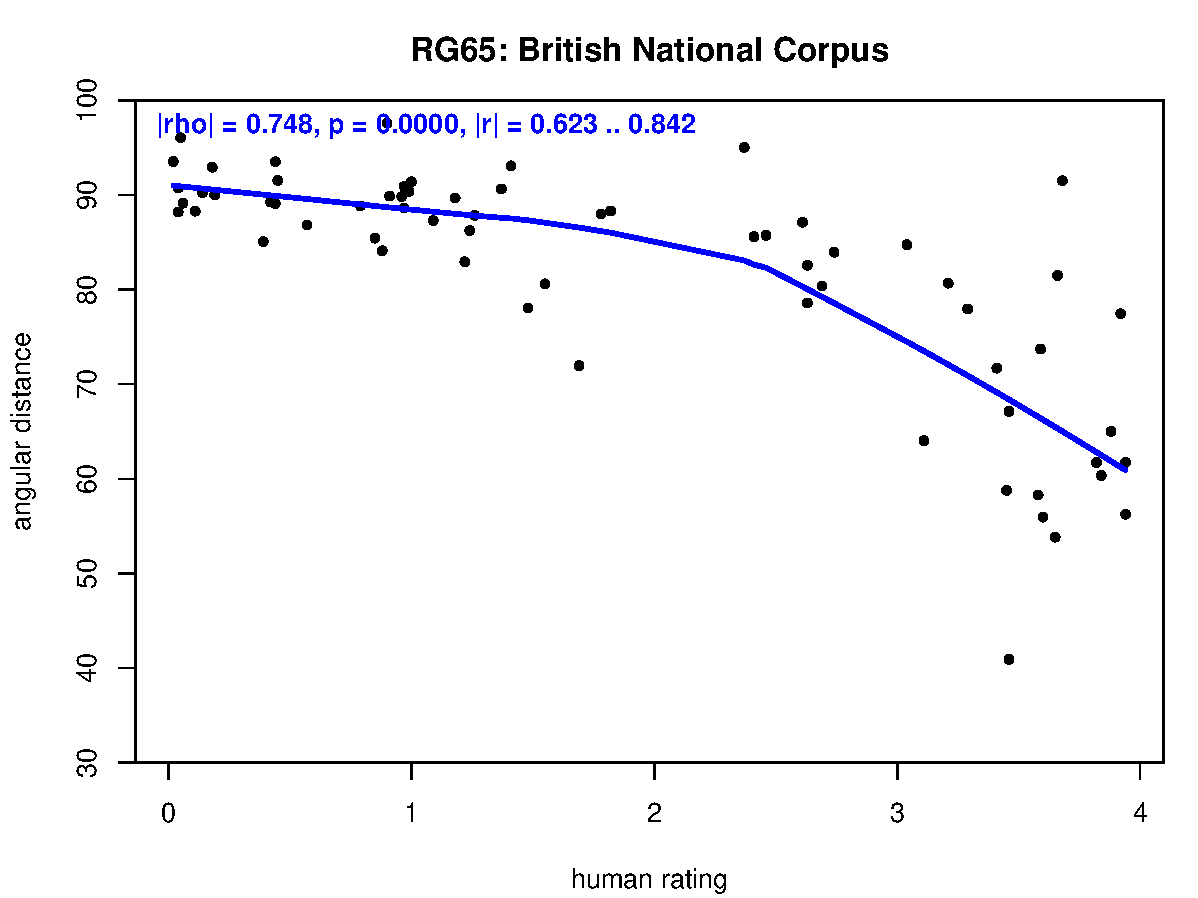
\includegraphics[width=10cm]{img/bnc_rg65}
  \end{center}
\end{frame}

\begin{frame}[fragile]
  \frametitle{Semantic similarity judgments: results}

  Results on RG65 task (Pearson):
  \begin{itemize}
  \item Dependency-filtered, BNC: Padó and Lapata (\citeyear{Pado:Lapata:07}): 0.62
  \item Dependency-filtered, Web data \citep{Herdagdelen:Erk:Baroni:09}
    \begin{itemize}
    \item without SVD reduction: 0.69
    \item with SVD reduction: 0.80
    \end{itemize}
  \item Dependency typed \citep{Baroni:Lenci:10}: 0.82
  \item Term-term + some magic \citep{Hassan:Mihalcea:11}: 0.86
  \end{itemize}

  \vfill
\begin{Rcode}[And you?]
> eval.similarity.correlation(RG65, M, convert=FALSE)\begin{Rout}
       rho  p.value missing     r r.lower r.upper
RG65 0.687 2.61e-10       0 0.678    0.52   0.791\end{Rout}
> plot(eval.similarity.correlation( \REM{cosine similarity}
       RG65, M, convert=FALSE, details=TRUE))
\end{Rcode}
\end{frame}


%%%%%%%%%%%%%%%%%%%%%%%%%%%%%%%%%%%%%%%%%%
\subsection{Noun categorisation}

\begin{frame}
  \frametitle{Noun categorisation}

  \begin{itemize}
  \item In \primary{categorisation tasks}, subjects are typically asked to assign experimental items -- objects, images, words -- to a given category or group items belonging to the same category
    \begin{itemize}
    \item categorisation requires an understanding of the relationship between the items in a category
    \end {itemize}
  \item Categorisation is a basic cognitive operation and a precondition of many further semantic tasks
    \begin{itemize}
    \item \primary{inference}
      \begin{itemize}
      \item if X is a CAR then X is a VEHICLE
      \end{itemize}
    \item \primary{compositionality}
      \begin{itemize}
      \item $\lambda y: \text{FOOD}\; \lambda x:\text{ANIMATE} \; \bigl[ eat(x,y) \bigr]$
      \end{itemize}
    \end{itemize}
  \item ``Chicken-and-egg'' problem for relationship of categorisation and similarity (cf.\ Goodman 1972, Medin et al.\ 1993)
  \end{itemize}
\end{frame}

\begin{frame}
  \frametitle{Noun categorisation: datasets}

  \ungap[1.5]
  \begin{columns}
    \begin{column}{0.5 \textwidth}
      \begin{exampleblock}{ESSLLI08 (on focus today)}
        \textbf{44 nouns, 6 classes} \\
        \textit{potato} $\Longrightarrow$ \textsc{green}  \\
        \textit{hammer} $\Longrightarrow$ \textsc{tool}  \\
        \textit{car} $\Longrightarrow$ \textsc{vehicle} \\
        \textit{peacock} $\Longrightarrow$ \textsc{bird}     
      \end{exampleblock}
      \begin{exampleblock}{Almuhareb \& Poesio}
        \textbf{402 nouns, 21 classes} \\
        \textit{day} $\Longrightarrow$ \textsc{time}   \\
        \textit{kiwi} $\Longrightarrow$ \textsc{fruit}  \\
        \textit{kitten} $\Longrightarrow$ \textsc{animal} \\
        \textit{volleyball} $\Longrightarrow$ \textsc{game}
      \end{exampleblock}
    \end{column}
    \begin{column}{0.5 \textwidth}
      \begin{exampleblock}{BATTIG set\phantom{p()} }
        \textbf{82 nouns, 10 classes} \\
        \textit{chicken} $\Longrightarrow$ \textsc{bird}   \\
        \textit{bear} $\Longrightarrow$ \textsc{land\_mammal}  \\
        \textit{pot} $\Longrightarrow$ \textsc{kitchenware} \\
        \textit{oak} $\Longrightarrow$ \textsc{tree}\phantom{p} 
      \end{exampleblock}
      \begin{exampleblock}{MITCHELL set \phantom{ \&}}
        \textbf{60 nouns, 12 classes} \\
        \textit{ant} $\Longrightarrow$ \textsc{insect}   \\
        \textit{carrot} $\Longrightarrow$ \textsc{vegetable}  \\
        \textit{train} $\Longrightarrow$ \textsc{vehicle} \\
        \textit{cat} $\Longrightarrow$ \textsc{animal}
      \end{exampleblock}
    \end{column}
  \end{columns}
\end{frame}

\begin{frame}[fragile]
  \frametitle{Noun categorisation: the ESSLLI 2008 dataset}

  Dataset of 44 concrete nouns (ESSLLI 2008 Shared Task)
  \begin{itemize}
  \item 24 natural entities
    \begin{itemize}
    \item 15 animals: 7 birds (\emph{eagle}), 8 ground animals (\emph{lion})
    \item 9 plants: 4 fruits (\emph{banana}), 5 greens (\emph{onion})
    \end{itemize}
  \item 20 artifacts
    \begin{itemize}
    \item 13 tools (\emph{hammer}), 7 vehicles (\emph{car})
    \item[]
    \end{itemize}
  \item<2-> DSMs operationalise categorisation as a \primary{clustering task}
    \begin{enumerate}
    \item for each noun $w_i$ in the dataset, take its vector $\vw_i$
    \item use a \primary{clustering method} to group similar vectors $\vw_i$
    \item evaluate whether clusters correspond to gold-standard semantic
      classes (purity, entropy, \ldots)
    \end{enumerate}
  \end{itemize}

  \vfill
\begin{Rcode}
> ESSLLI08_Nouns[seq(1,40,5), ]
\end{Rcode}
\end{frame}


\begin{frame}
\frametitle{Noun categorisation: example}
\ungap[1]
\begin{center}
  \only<beamer:1| handout:0>{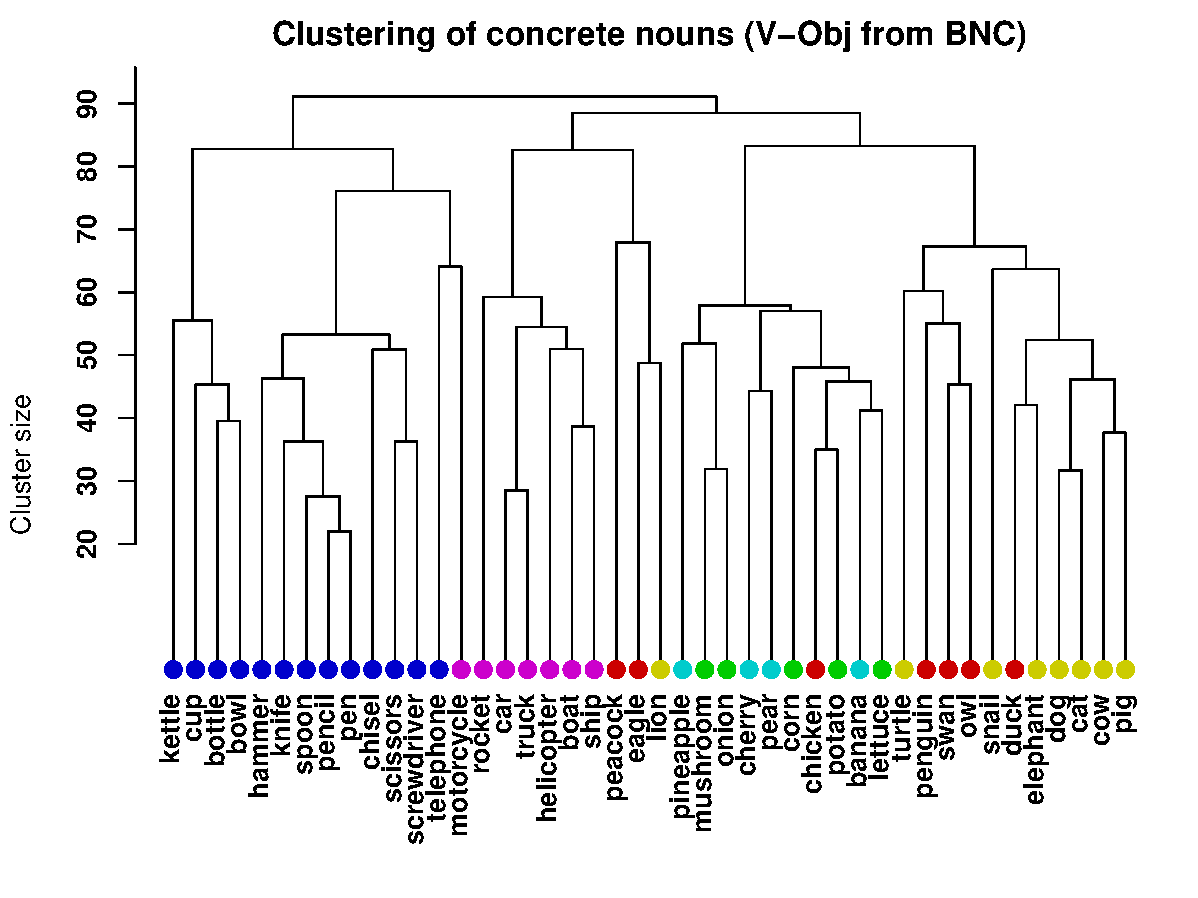
\includegraphics[width=8cm]{img/vobj_clustering}}%
  \only<beamer:2-| handout:1>{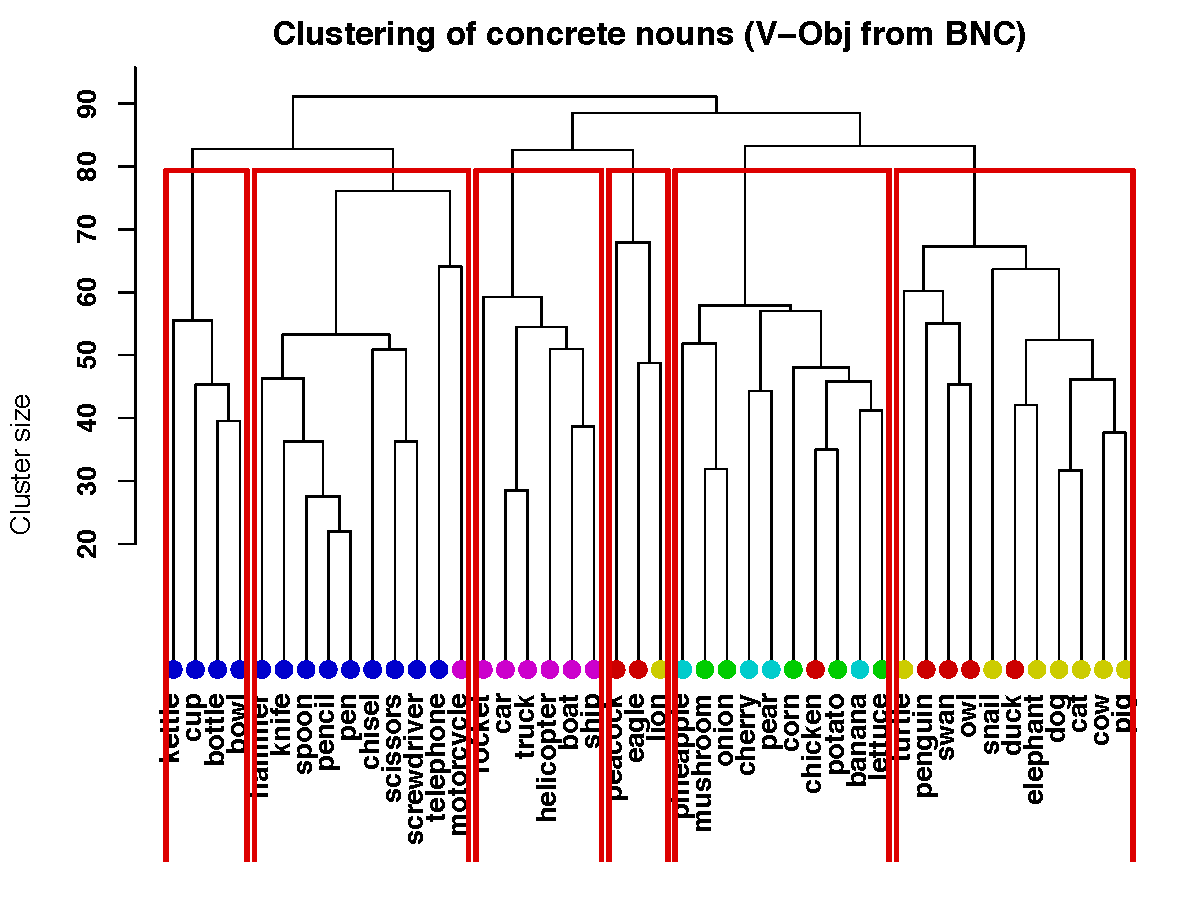
\includegraphics[width=8cm]{img/vobj_clustering_6}}%
\end{center}
\ungap[1]
\begin{itemize}
\item<3-> majority labels: {\color{pureblue}tools}, {\color{pureblue}tools}, {\color[rgb]{.7, .1, .7}vehicles}, {\color{purered}birds}, {\color{puregreen}greens}, {\color[rgb]{.7, .6, .1}animals}
\item<3-> correct: 4/4, 9/10, 6/6, 2/3, 5/10, 7/11
\item<4-> purity = 33 correct out of 44 = 75.0\%
\end{itemize}
\end{frame}

\begin{frame}
  \frametitle{ESSLLI 2008 shared task}
  \begin{itemize}
  \item Clustering experiments with CLUTO \citep{Karypis:03}
  \item[]
    \begin{itemize}
    \item 6-way (birds, ground animals, fruits, greens,
      tools and vehicles), 3-way (animals, plants and
      artifacts) and 2-way (natural and artificial entities) clusterings
    \end{itemize}
    \pause
  \item Evaluation scores:
    \begin{itemize}
    \item \h{purity} -- degree to which a cluster contains words from one class only (\secondary{best = 1})
    \item \primary{entropy} -- whether words from different classes are represented in the same cluster (\secondary{best = 0})
    \item \primary{global score} across the three clustering experiments
      \begin{displaymath}
        \sum_{i=1}^3 \text{Purity}_i -  \sum_{i=1}^3 \text{Entropy}_i
      \end{displaymath}
    \end{itemize}
  \end{itemize}
\end{frame}

\begin{frame}[fragile]
  \frametitle{ESSLLI 2008 shared task}

  \begin{center}\small
    \begin{tabular}{|l|r|r||r|r||r|r||r|}
      \hline
      \emph{model} &\multicolumn{2}{|c||}{\emph{6-way}} &  \multicolumn{2}{|c||}{\emph{3-way}} & \multicolumn{2}{|c||}{\emph{2-way}}&  \multicolumn{1}{|c|}{\emph{global}}\\
      \cline{2-7}
                   &   \emph{P} & \emph{E}  & \emph{P} & \emph{E}  & \emph{P} & \emph{E} &\\
      \hline
      \hline
      Pattern-based (Katrenko) & 89 & 13 & 100 & 0 & 80 & 59 & 197\\ 
      \hline
      Term-term (Peirsman) & 82 & 23 & 84 & 34 & 86 & 55 & 140\\
      \hline
      dep-typed (DM) & 77 & 24 & 79 & 38 & 59 & 97 & 56\\
      \hline
      dep-filtered (DM) & 80 &28 & 75& 51& 61& 95 & 42\\
      \hline
      window (DM) & 75& 27&  68& 51& 68& 89   &44\\
      %\hline
      %Peirsman$-$ & 73 & 28 & 71 & 54 & 61 & 96 & 27\\
      %\hline
      %Shaoul & 41& 77& 52& 84 & 55& 93& -106\\
      \hline
    \end{tabular}
  \end{center}

  \begin{center}\footnotesize
    {\tt Katrenko, Peirsman}: ESSLLI 2008 Shared Task\\
    {\tt DM}: Baroni \& Lenci (2009)
  \end{center}

  \vfill
\begin{Rcode}[And you?]
> eval.clustering(ESSLLI08_Nouns, M) \REM{uses PAM clustering}
\end{Rcode}
\end{frame}


%%%%%%%%%%%%%%%%%%%%%%%%%%%%%%%%%%%%%%%%%%
\subsection{Analogy}

\begin{frame}
  \frametitle{Intrinsic evaluation on word pairs: Analogy}
  \framesubtitle{\citet{Mikolov:etc:13,Mikolov:etc:13b,Gladkova:Drozd:Matsuoka:16}}

  \begin{itemize}
  \item Task: solve analogy problems such as
    \begin{itemize}
    \item \emph{man}$\,:\,$\emph{woman} $\;::\;$ \emph{king}$\,:\,$\only<beamer:1| handout:0>{\h{???}}\only<beamer:2-| handout:1>{\primary{\emph{queen}}}
    \item<2-> \emph{France}$\,:\,$\emph{Paris} $\;::\;$ \emph{Bulgaria}$\,:\,$\only<beamer:2| handout:0>{\h{???}}\only<beamer:3-| handout:1>{\primary{\emph{Sofia}}}
    \item<3-> \emph{learn}$\,:\,$\emph{learned} $\;::\;$ \emph{go}$\,:\,$\only<beamer:3| handout:0>{\h{???}}\only<beamer:4-| handout:1>{\primary{\emph{went}}}
    \item<4-> \emph{dog}$\,:\,$\emph{animal} $\;::\;$ \emph{strawberry}$\,:\,$\only<beamer:4| handout:0>{\h{???}}\only<beamer:5-| handout:1>{\primary{\emph{fruit}}}
    \item[]
    \end{itemize}
  \item<6-> Approach 1: build DSM on word pairs as targets
    \[
      \min_{x}\, \dist{\vv_{\text{man:woman}}}{\vv_{\text{king:$x$}}}
    \]
  \item<7-> Approach 2: use vector operations in single-word DSM
    \begin{tikzpicture}
      \useasboundingbox (.8, 1.5) rectangle (1, 1.7) ;
      \node (woman) at (0, 1) {\hh{\small woman}} ;
      \node (man) at (1, 0) {\hh{\small man}} ;
      \node (king) at (2, 1.5) {\hh{\small king}} ;
      \node (queen) at (1, 2.5) {\hh{\small queen}} ;
      \draw[diagram arrow=primary] (man) -- (woman) ;
      \draw[diagram arrow=primary] (king) -- (queen) ;
      \draw[diagram arrow=counterpoint] (man) -- (king) ;
    \end{tikzpicture}
    \[
      \vv_{\text{queen}} \approx \vv_{\text{king}} - \vv_{\text{man}} + \vv_{\text{woman}}
    \]
  \end{itemize}
\end{frame}

\begin{frame}
  \frametitle{The Google analogy task}
  \framesubtitle{\citet{Mikolov:etc:13,Mikolov:etc:13b}}

  \begin{center}
    \ungap[1]
    \begin{tabular}{r}
      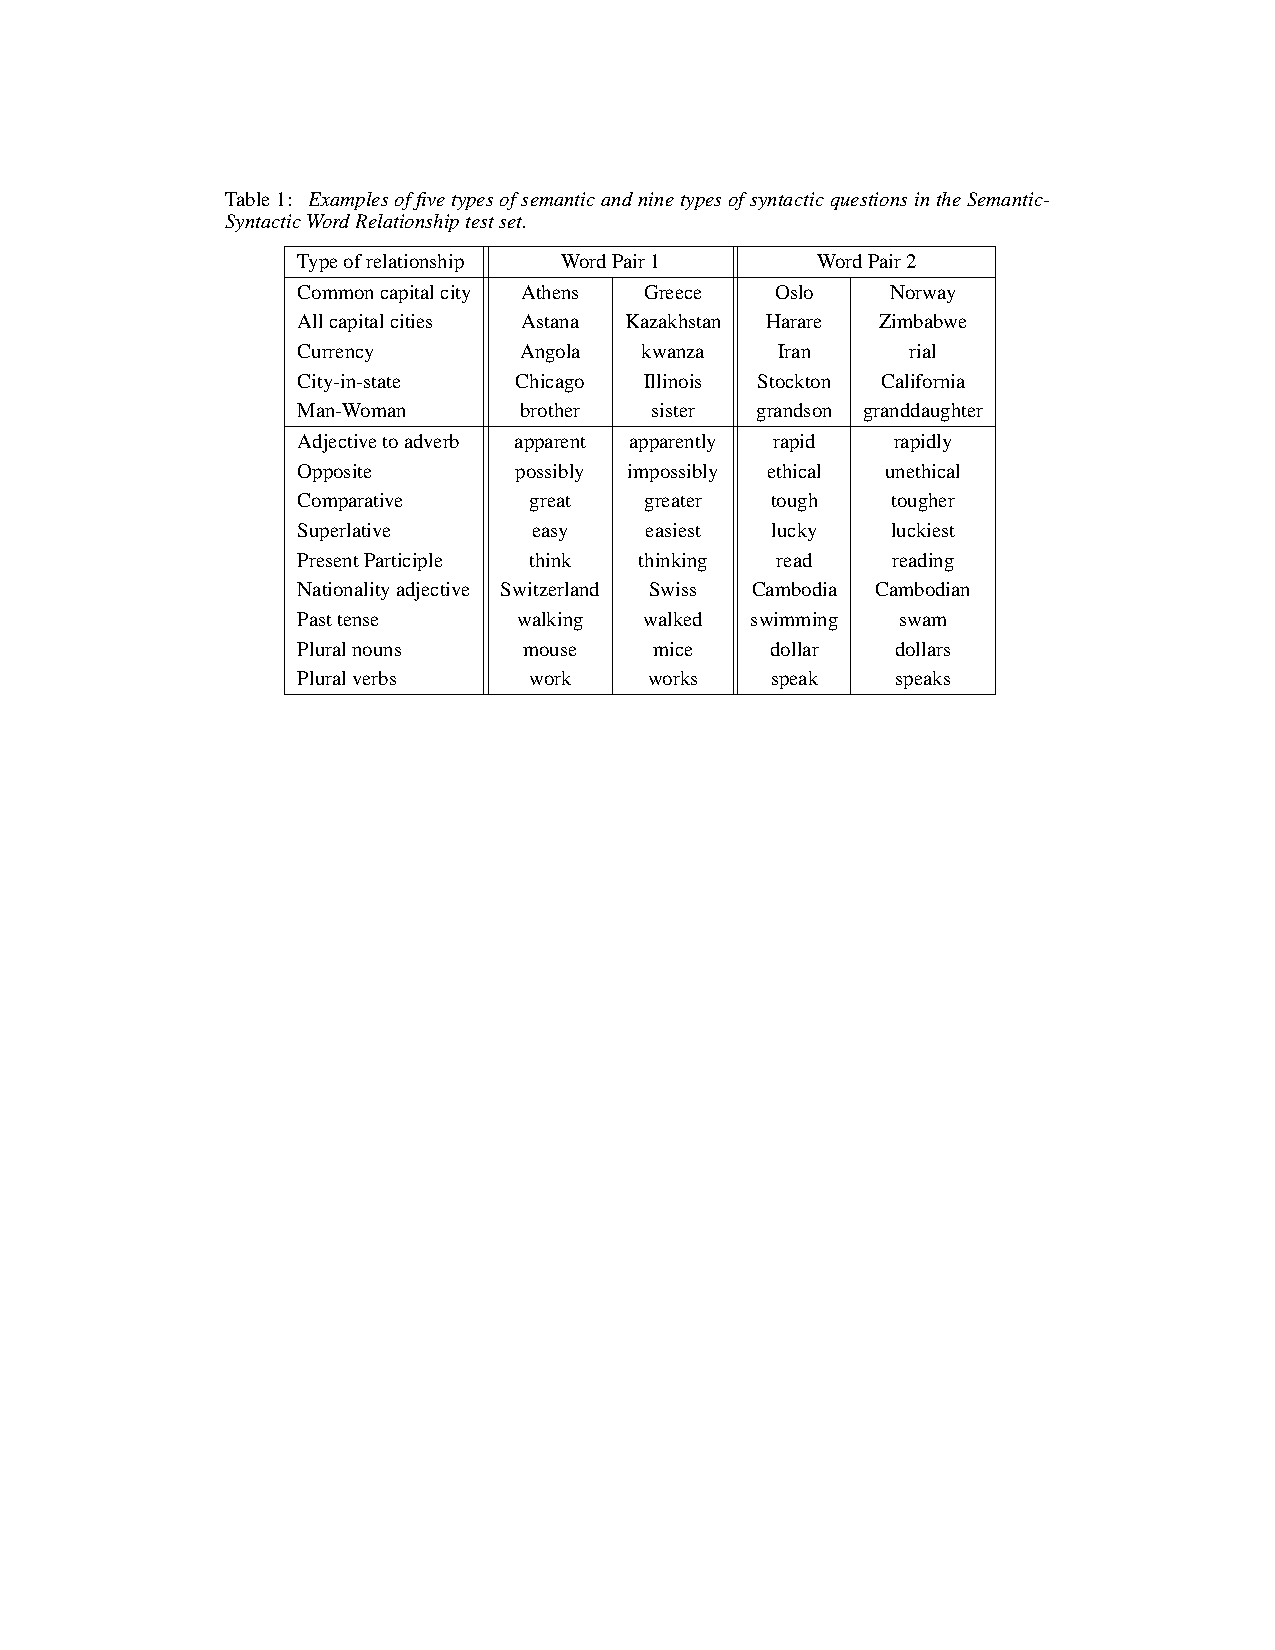
\includegraphics[width=10cm]{img/MikolovChenEtc2013_Tab1}\\
      \secondary{\tiny\citep[Tab.~1]{Mikolov:etc:13}}
    \end{tabular}
  \end{center}
\end{frame}

\begin{frame}
  \frametitle{The Google analogy task}
  \framesubtitle{\citet{Mikolov:etc:13,Mikolov:etc:13b}}

  \begin{columns}[c]
    \begin{column}{5cm}
      \begin{itemize}
      \item \citet{Mikolov:etc:13,Mikolov:etc:13b} claim that their neural
        embeddings are good at solving analogy tasks
      \item[\So] Semantic features encoded in linear subdimensions
      \end{itemize}
    \end{column}
    \begin{column}{55mm}
      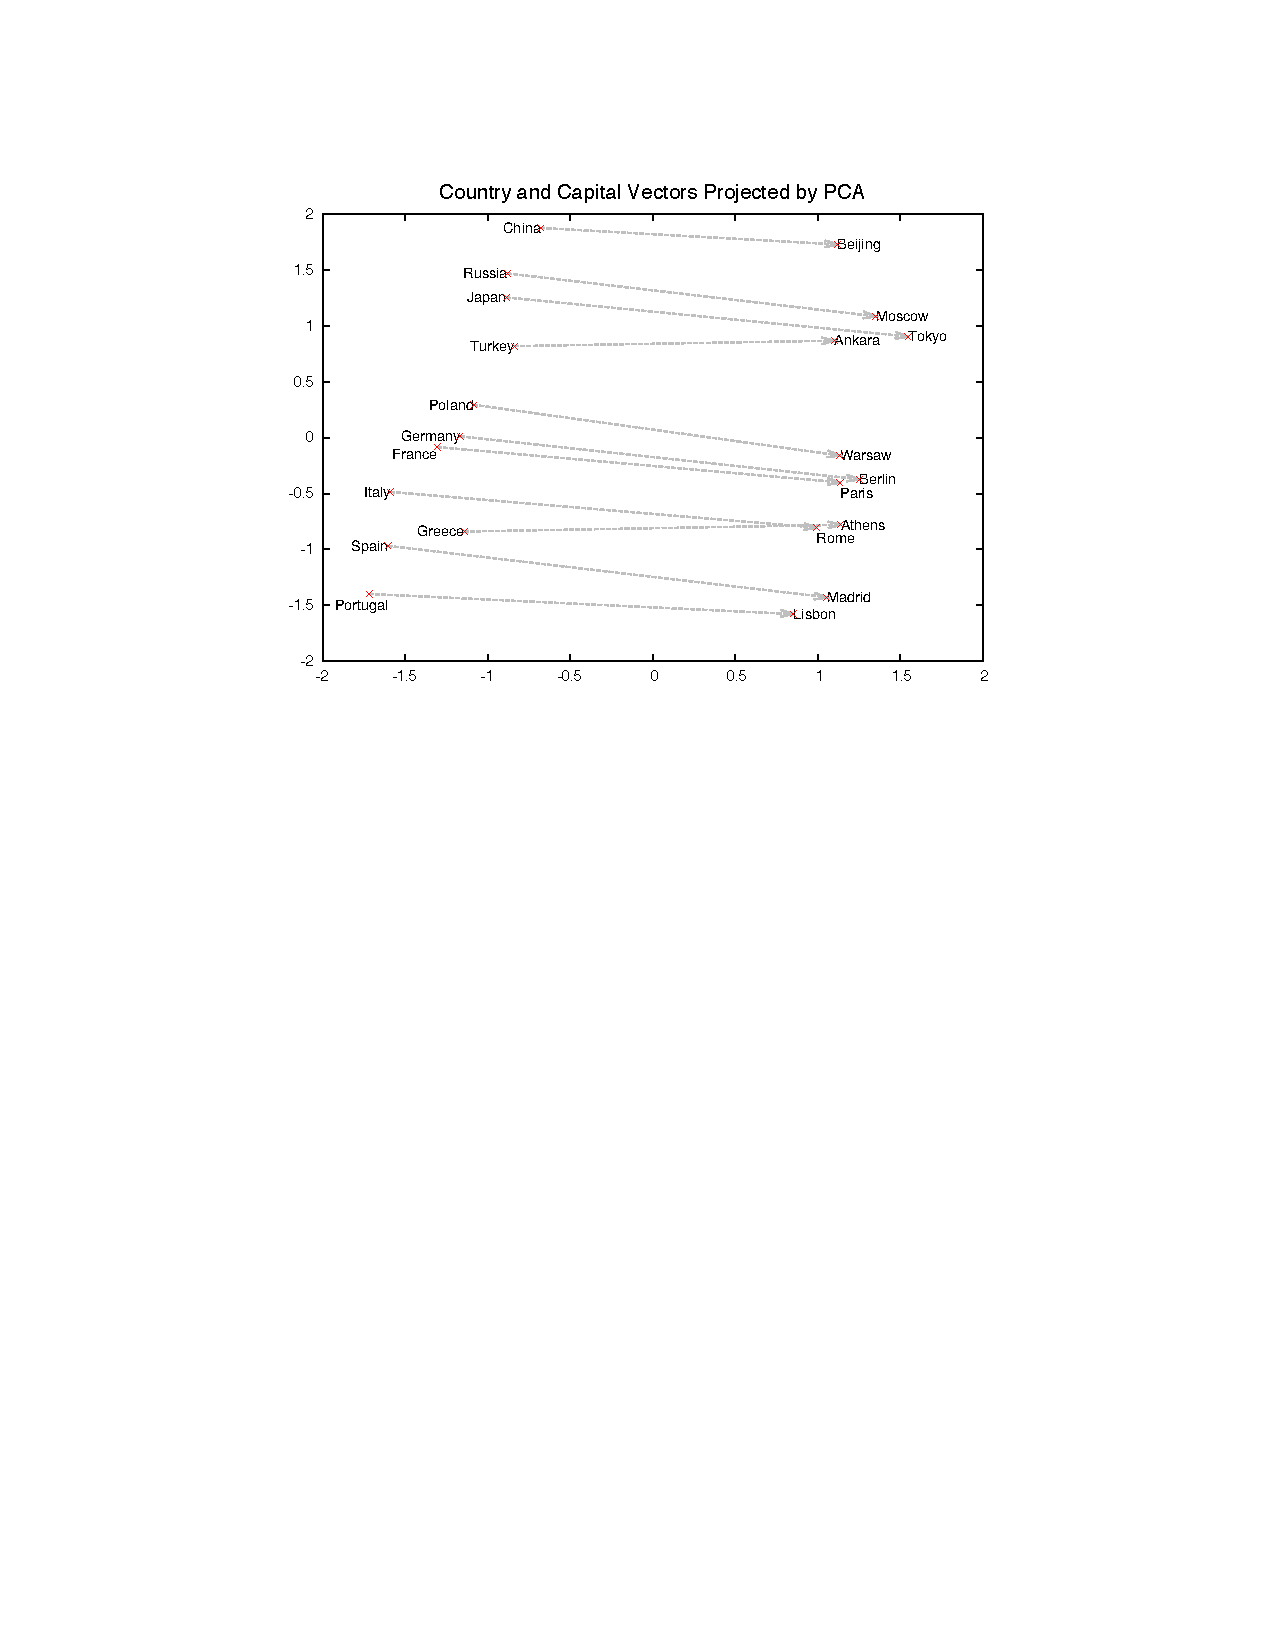
\includegraphics[width=55mm]{img/MikolovSutskeverEtc2013_Fig2}\\
      \tiny\hfill\secondary{\citep[Fig.~2]{Mikolov:etc:13b}}
    \end{column}
  \end{columns}

  \onslide<2->
  \begin{center}
    \begin{tabular}{>{\secondary}lccl}
      model & syntactic & semantic & \\
      \toprule
      word2vec & 64\% & 55\% & \citep{Mikolov:etc:13} \\
      DSM & 43\% & 60\% & \citep{Baroni:Dinu:Kruszewski:14} \\
      FastText & 82\% & 87\% & \citep{Mikolov:etc:18}
    \end{tabular}
  \end{center}
\end{frame}

\begin{frame}
  \frametitle{Scaling up: Linguistic Diagnostics}

  \begin{columns}[T]
    \begin{column}{45mm}
      \primary{Linguistic Diagnostics} \citep{Rogers:Hosur:Rumshisky:18} automates classification of nearest neighbours based on various on-line dictionaries and semantic networks
      \begin{itemize}
      \item[\hand] correlation analysis between various groups of diagnostics and evaluation tasks
      \item[\hand] only for English so far
      \end{itemize}
    \end{column}
    \begin{column}{65mm}
      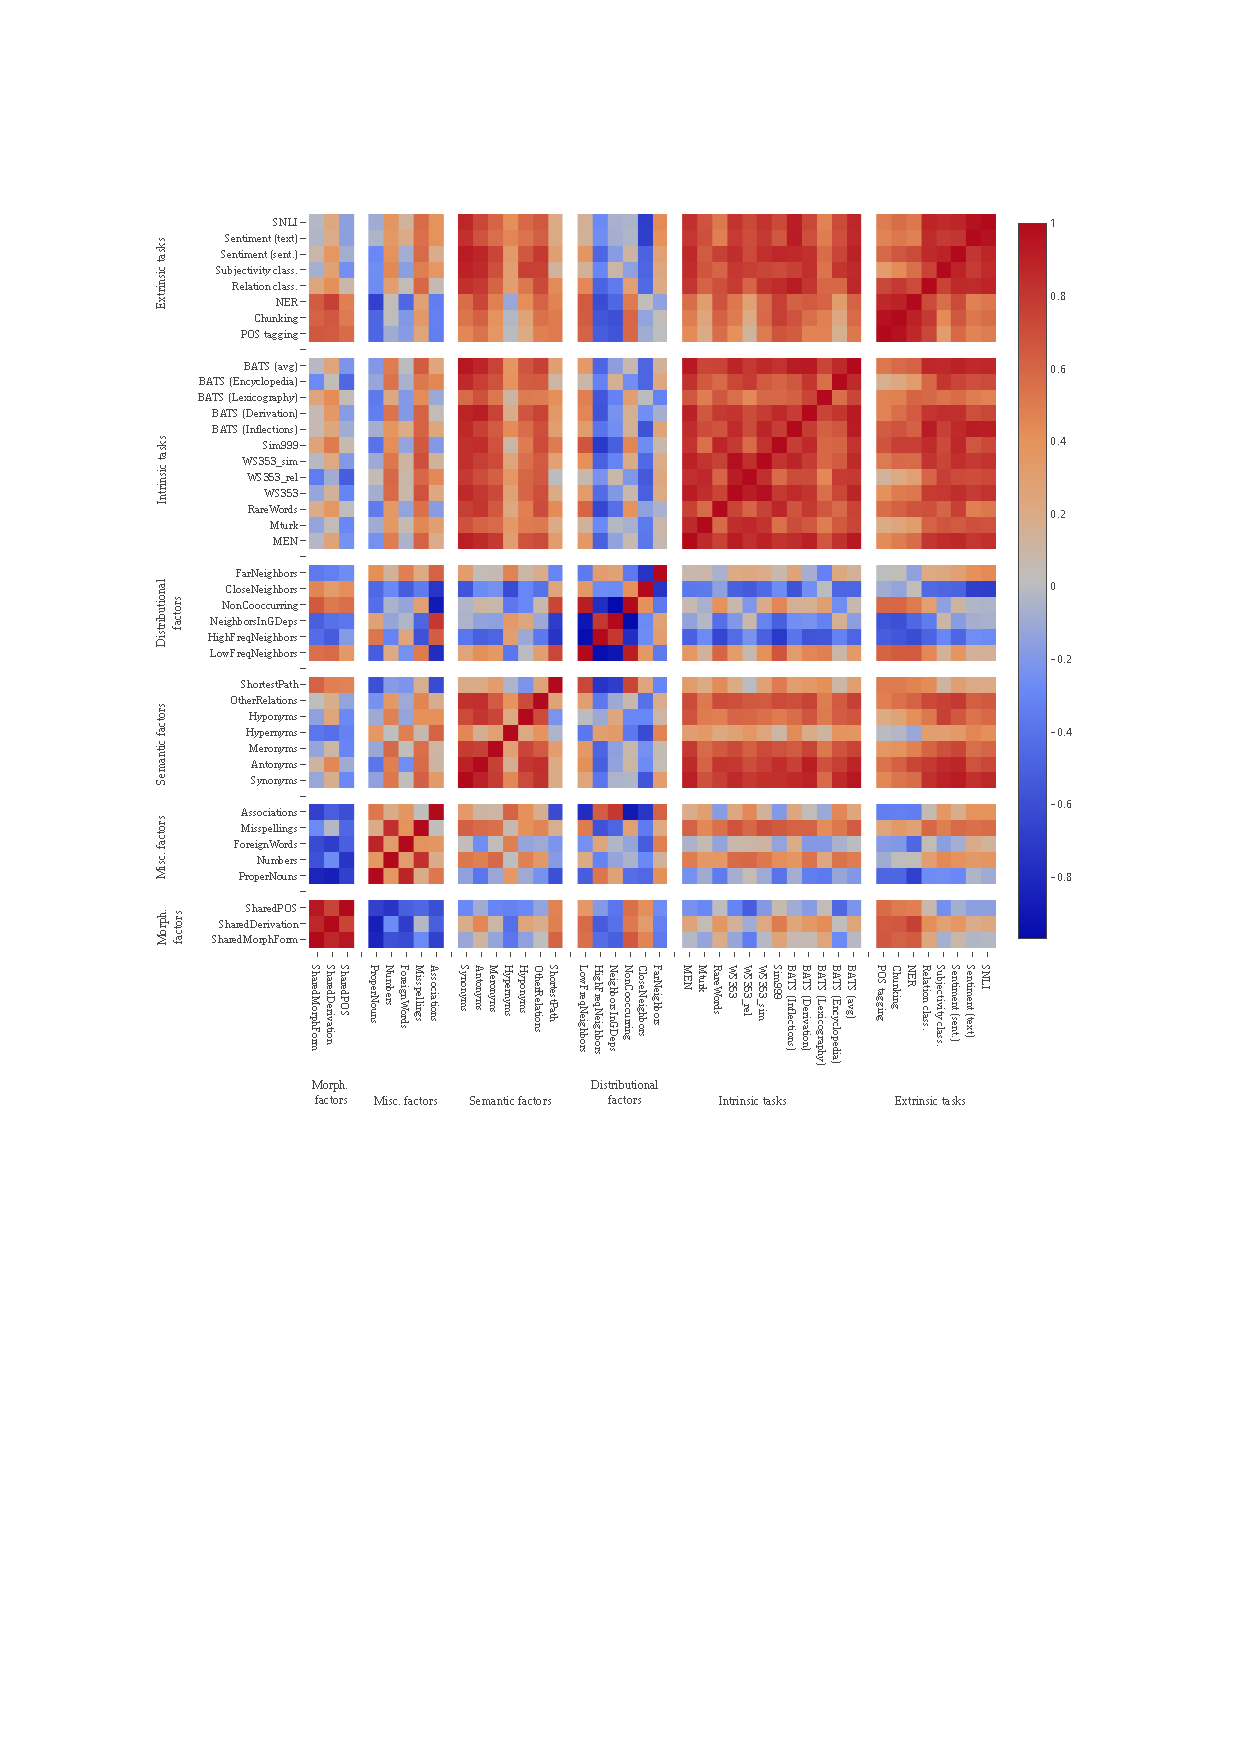
\includegraphics[width=65mm]{img/RogersEtc2018_Fig2}%
    \end{column}
  \end{columns}
  \gap[.5]
  \hspace*{-3mm}\secondary{\small\url{https://github.com/annargrs/ldt}}
\end{frame}


%%%%%%%%%%%%%%%%%%%%%%%%%%%%%%%%%%%%%%%%%%%%%%%%%%%%%%%%%%%%%%%%%%%%%% 
\section{Methodology for evaluation of DSM parameters}

%%%%%%%%%%%%%%%%%%%%%%%%%%%%%%%%%%%%%%%%%%
\subsection{An example (Bullinaria \& Levy 2007, 2012)}

\begin{frame}
  \frametitle{DSM evaluation in published studies}

  \begin{itemize}
  \item \primary{One model, many tasks} \citep{Pado:Lapata:07,Baroni:Lenci:10,Pennington:Socher:Manning:14}
    \begin{itemize}
    \item A novel DSM is proposed, with specific features \& parameters
    \item This DSM is tested on a range of different tasks\\ (e.g.\ TOEFL, priming, semantic clustering)
    \item[]
    \end{itemize}

  \item<2-> \primary{Incremental tuning of parameters} \citep{Bullinaria:Levy:07,Bullinaria:Levy:12,Kiela:Clark:14,Polajnar:Clark:14}
    \begin{itemize}
    \item Several parameters (e.g., scoring measure, distance metric, dimensionality reduction) 
    \item Many tasks (e.g.\ TOEFL, semantic \& syntactic clustering)
    \item Varying granularity of parameter settings
    \item One parameter (sometimes two) varied at a time, with all other parameters set to fixed values or optimized for each setting
    \item Optimal parameter values are determined sequentially
    \end{itemize}
  \end{itemize}
\end{frame}

\begin{frame}
  \frametitle{\citet{Bullinaria:Levy:07,Bullinaria:Levy:12}}
  
  \ungap[1]
  \begin{itemize}
  \item One of the first systematic evaluation studies
  \item Test influence of many standard parameter settings
    \begin{itemize}
    \item frequency weighting + distance measure
    \item co-occurrence window, structured \vs unstructured
    \item corpus type \& size, number of feature dimensions
    \item dimensionality reduction (SVD), number of latent dimension
    \end{itemize}
  \item<2-> In five different evaluation tasks
    \begin{itemize}
    \item TOEFL
    \item distance comparison: related word \vs 10 random words
    \item semantic categorisation: nearest-centroid classifier
    \item syntactic categorisation (2007)
    \item semantic clustering of nouns (2012)
    \end{itemize}
  \item<3-> Novel parameters
    \begin{itemize}
    \item skipping of first latent dimensions (with highest variance)
    \item Caron's (\citeyear{Caron:01}) $P$: power-scaling of singular values
    \end{itemize}
  \end{itemize}
\addnote{Note that B\&L do not test all commonly used parameter settings, e.g.\ log-likelihood or log frequency as feature weighting.}%
\addnote{They also do not seem to normalize row vectors properly (frequency vectors are scaled to probabilities, i.e.\ $\norm[1]{x} = 1$), which might explain the poor results from Euclidean distance.}%
\addnote{Noun clustering uses \citet{Mitchell:etc:08} dataset of 60 nouns from 12 categories, and CLUTO direct clustering with standard settings.}%
\addnote{Incremental approach also across the two studies: B\&L (2012) builds on and extends results of B\&L (2007).}%
\addnote{Note that B\&L's power scaling notation differs from \citet{Caron:01}: $P = 1 + p/2$}%
\end{frame}

\begin{frame}
  \frametitle{TOEFL results: feature weighting \& distance measure}
  \framesubtitle{\citep[p.~516, Fig.~1]{Bullinaria:Levy:07}}

  \ungap[1.5]
  \begin{center}
    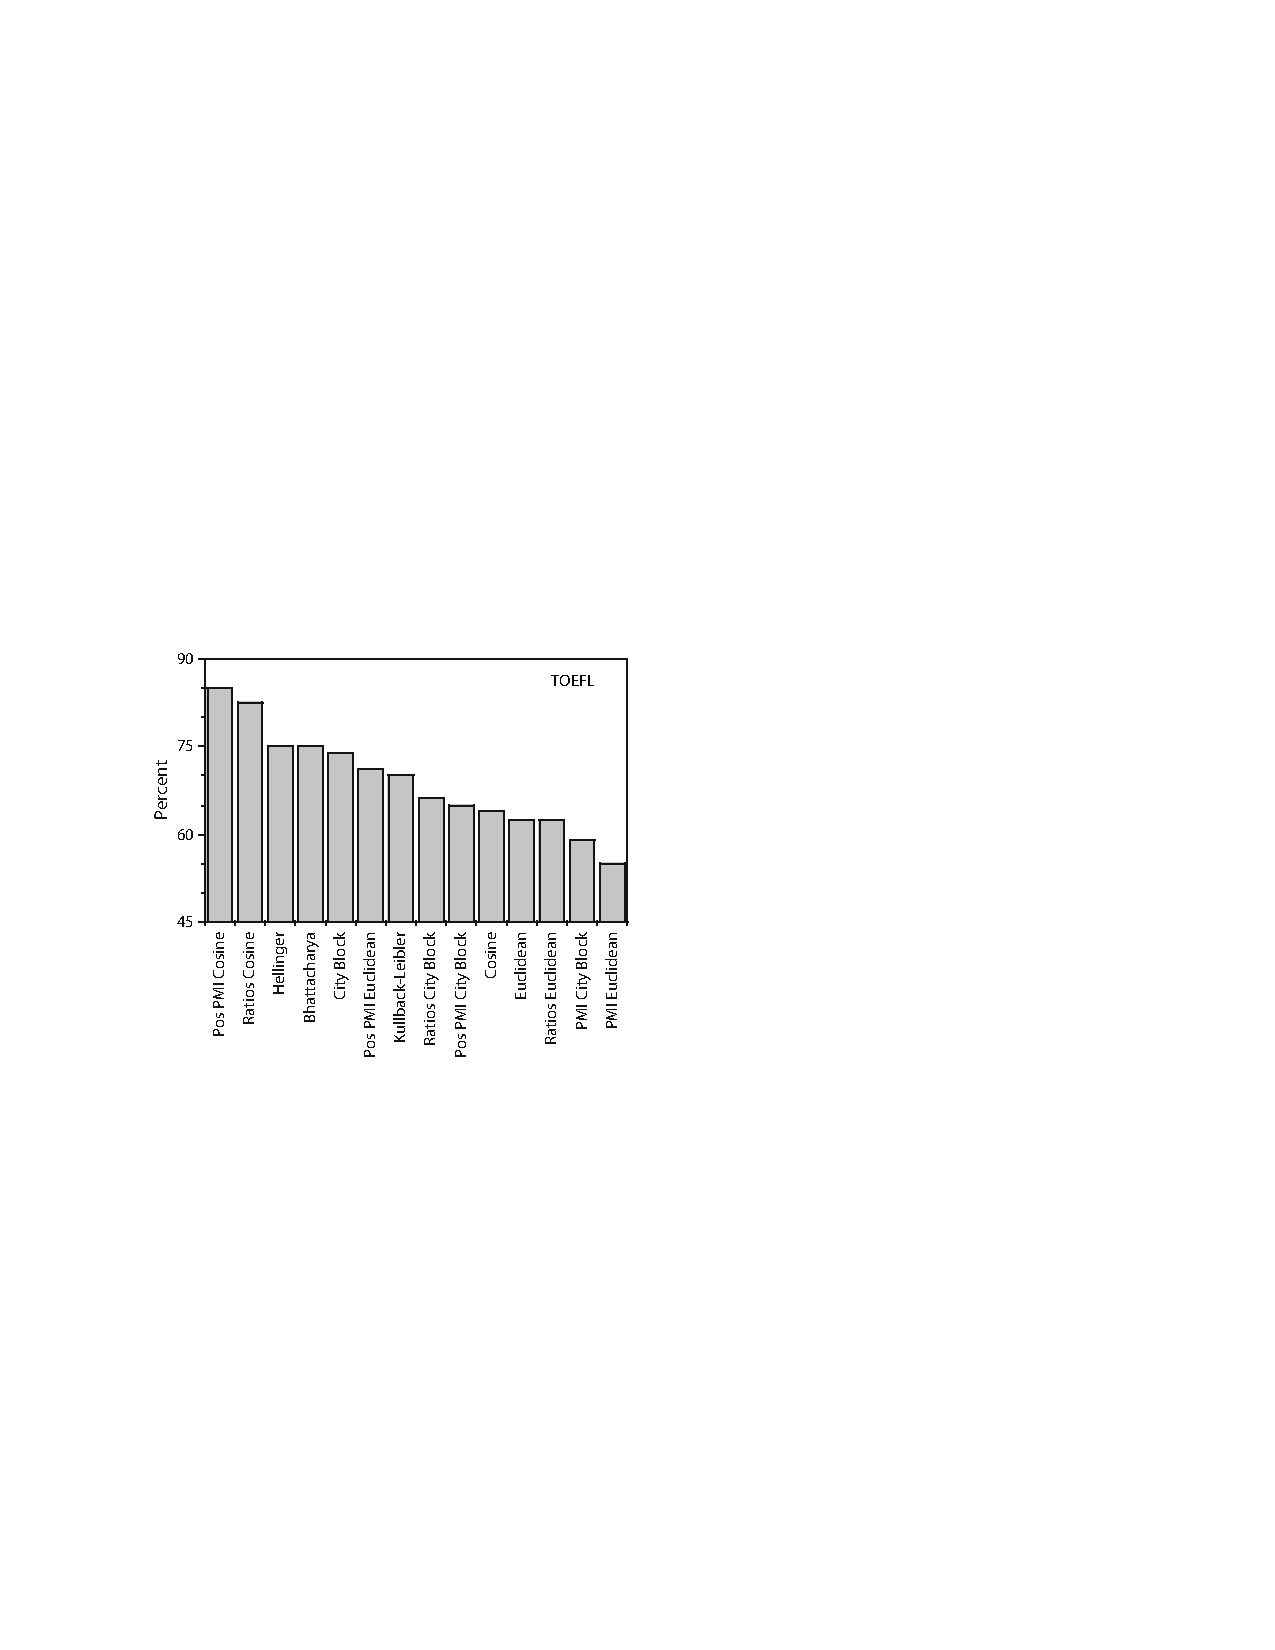
\includegraphics[width=7cm]{img/BullinariaLevy2007_p516_fig1_TOEFL_metric}
  \end{center}

  \ungap[1]
  \secondary{\scriptsize
   British National Corpus (BNC). Vectors not L2-normalized (frequency is L1-normalized). All other parameters optimized for each setting.
    \par% terminate paragraph to recompute line spacing while \scriptsize is still in effect
  }
\end{frame}

\begin{frame}
  \frametitle{TOEFL results: size \& type of co-occurrence window}
  \framesubtitle{\citep[p.~893, Fig.~1]{Bullinaria:Levy:12}}

  \ungap[1]
  \begin{center}
    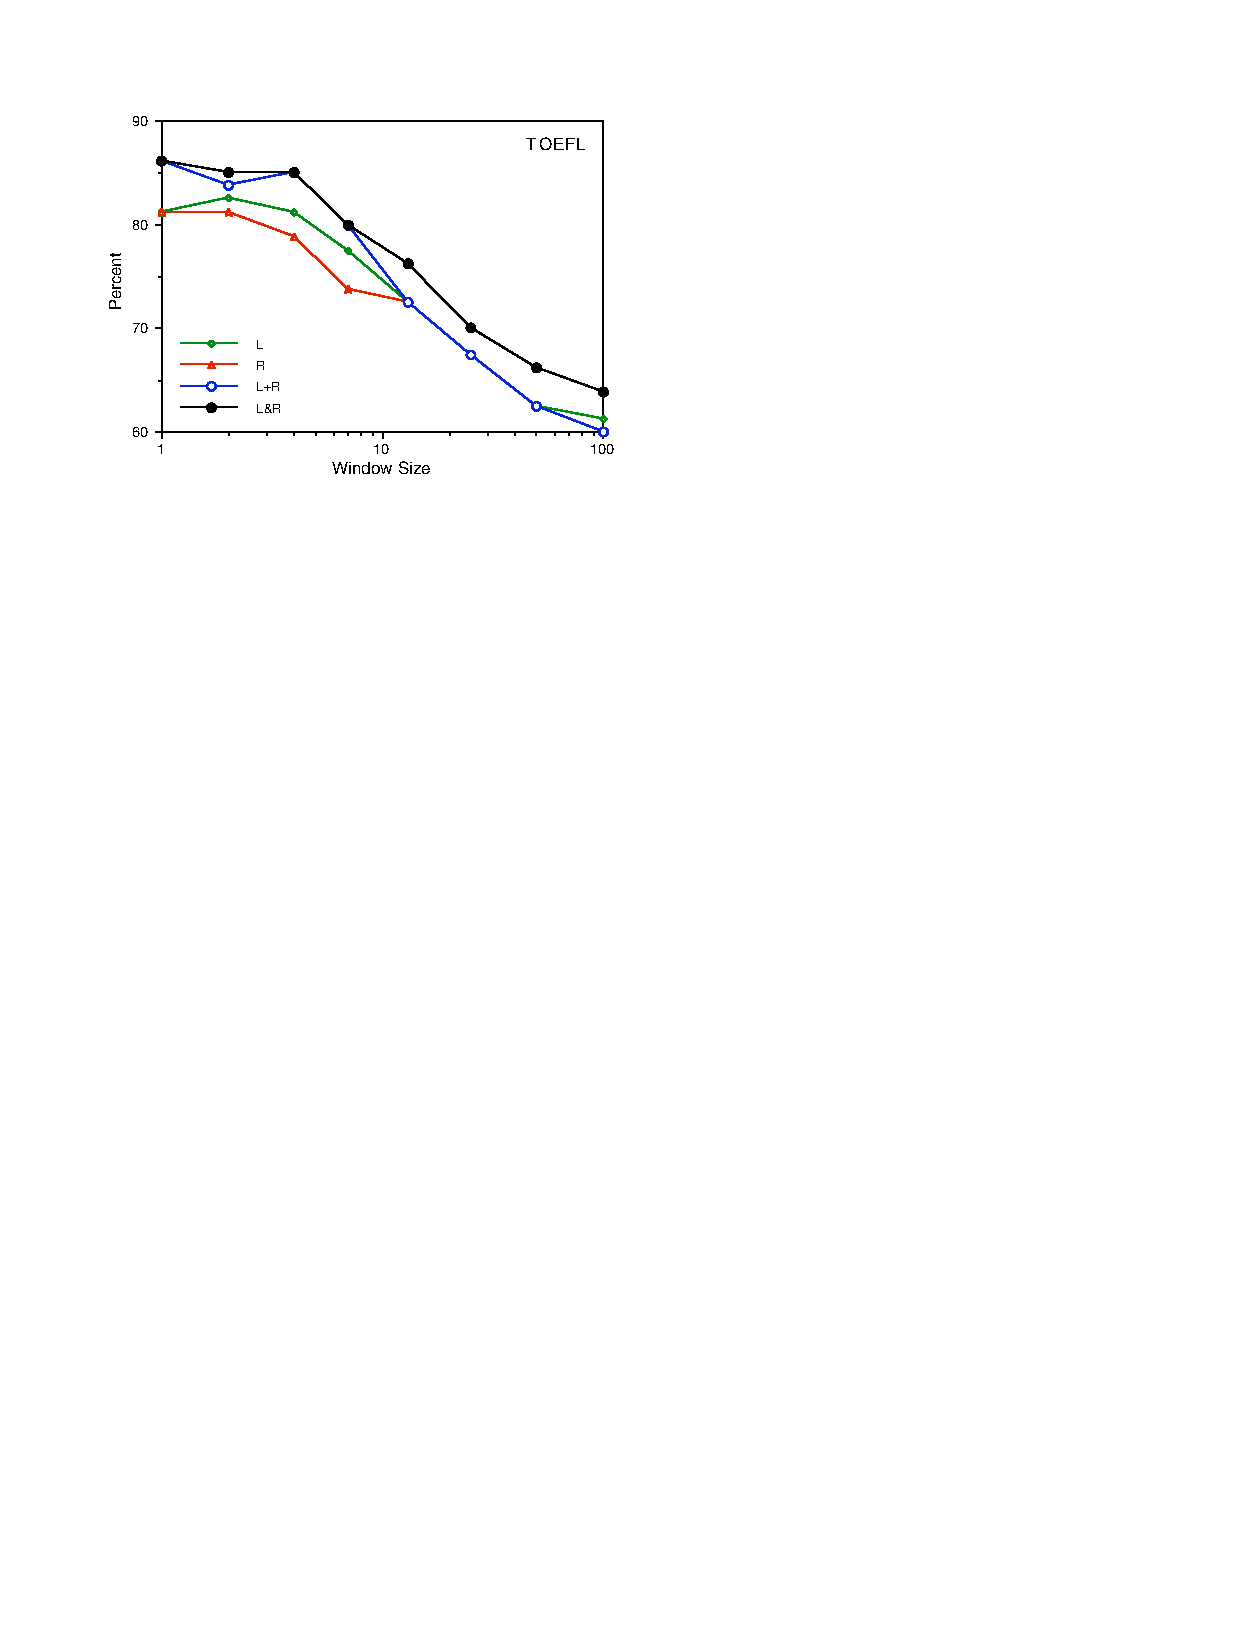
\includegraphics[width=8cm]{img/BullinariaLevy2012_p893_fig1_TOEFL_window}
  \end{center}

  \ungap[.5]
  \secondary{\scriptsize
    ukWaC Web corpus. Positive PMI + cosine \citep{Bullinaria:Levy:07}. Number of feature dimensions optimized for each window size \& task. No dimensionality reduction. L\&R = structured surface context (left/right).
    \par%
  }
\end{frame}

\begin{frame}
  \frametitle{TOEFL results: corpus type \& size}
  \framesubtitle{\citep[p.~894, Fig.~2]{Bullinaria:Levy:12}}

  \ungap[1]
  \begin{center}
    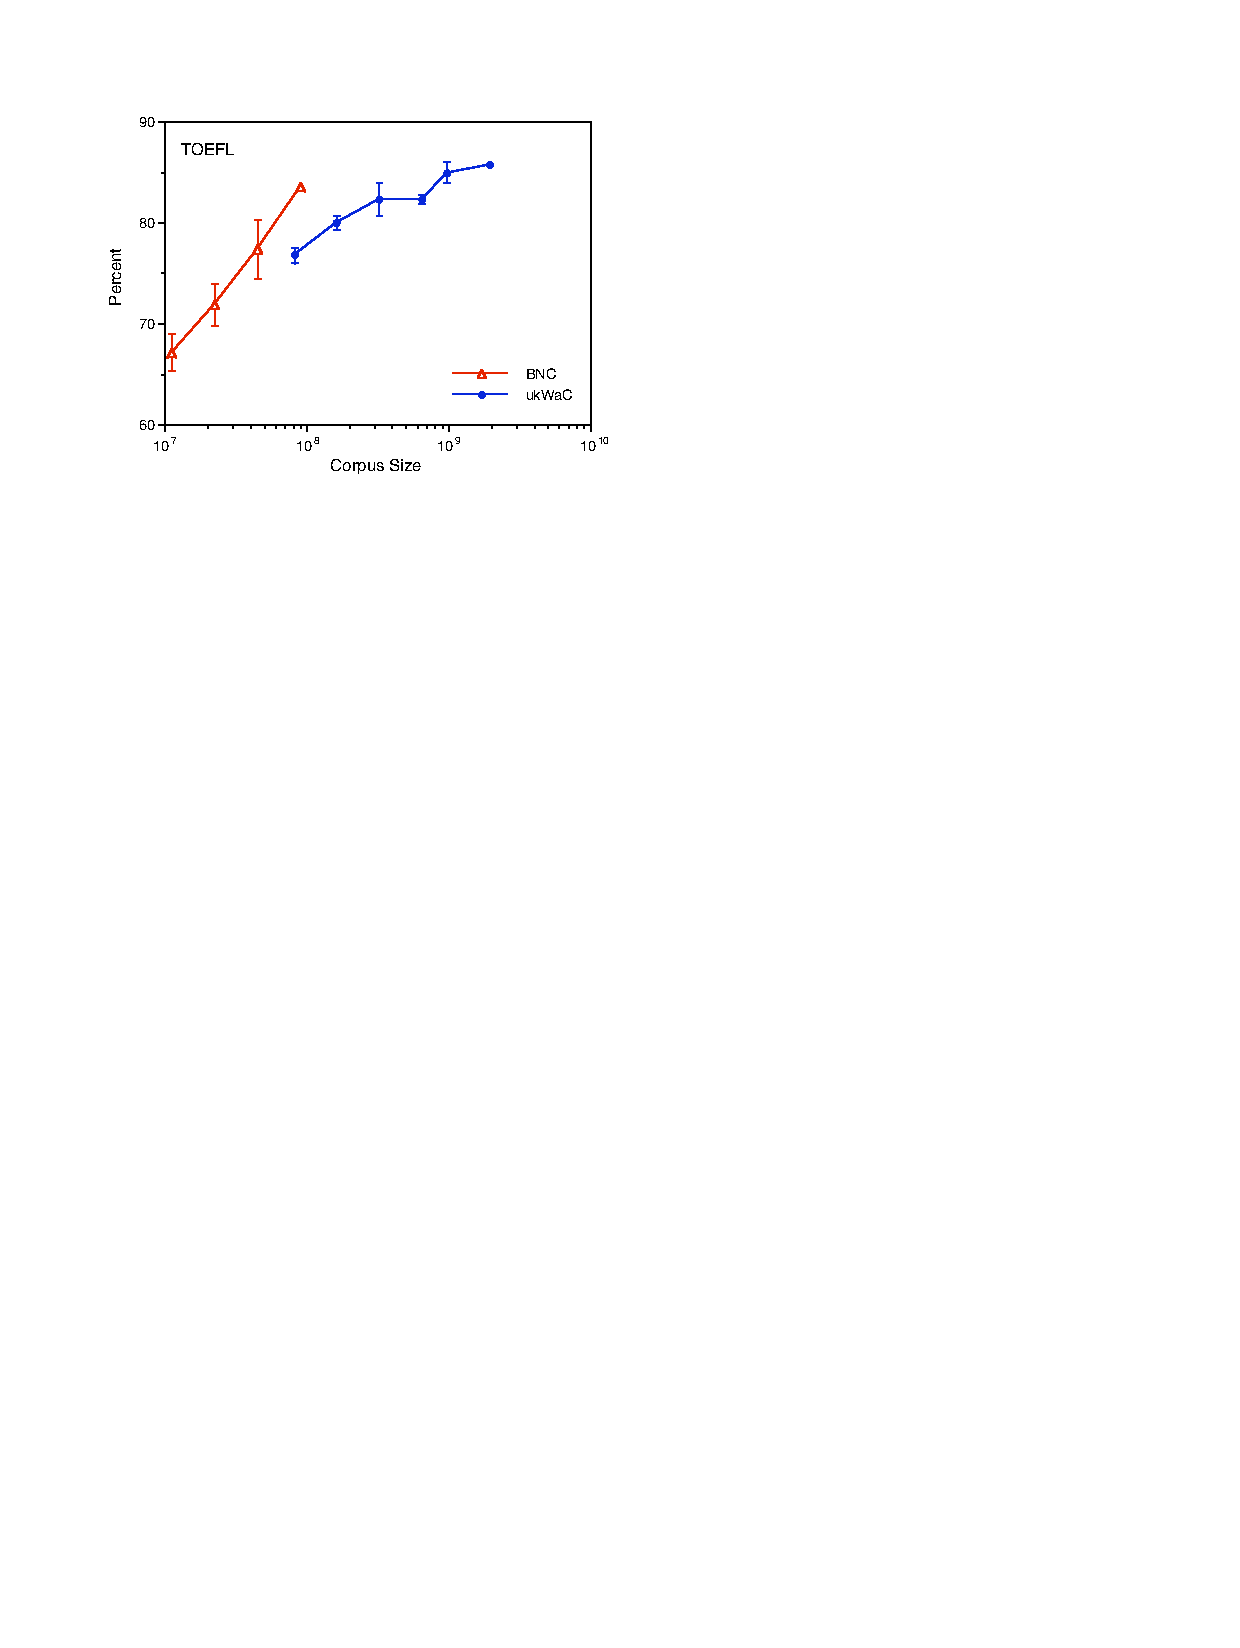
\includegraphics[width=8cm]{img/BullinariaLevy2012_p894_fig2_TOEFL_size}
  \end{center}

  \ungap[.5]
  \secondary{\scriptsize
    L+R context of size 1. Average + standard error over equally-sized corpus slices. Other parameter settings unclear.
    \par%
  }
\end{frame}

\begin{frame}
  \frametitle{TOEFL results: feature dimensions \& pre-processing}
  \framesubtitle{\citep[p.~895, Fig.~4]{Bullinaria:Levy:12}}

  \ungap[1]
  \begin{center}
    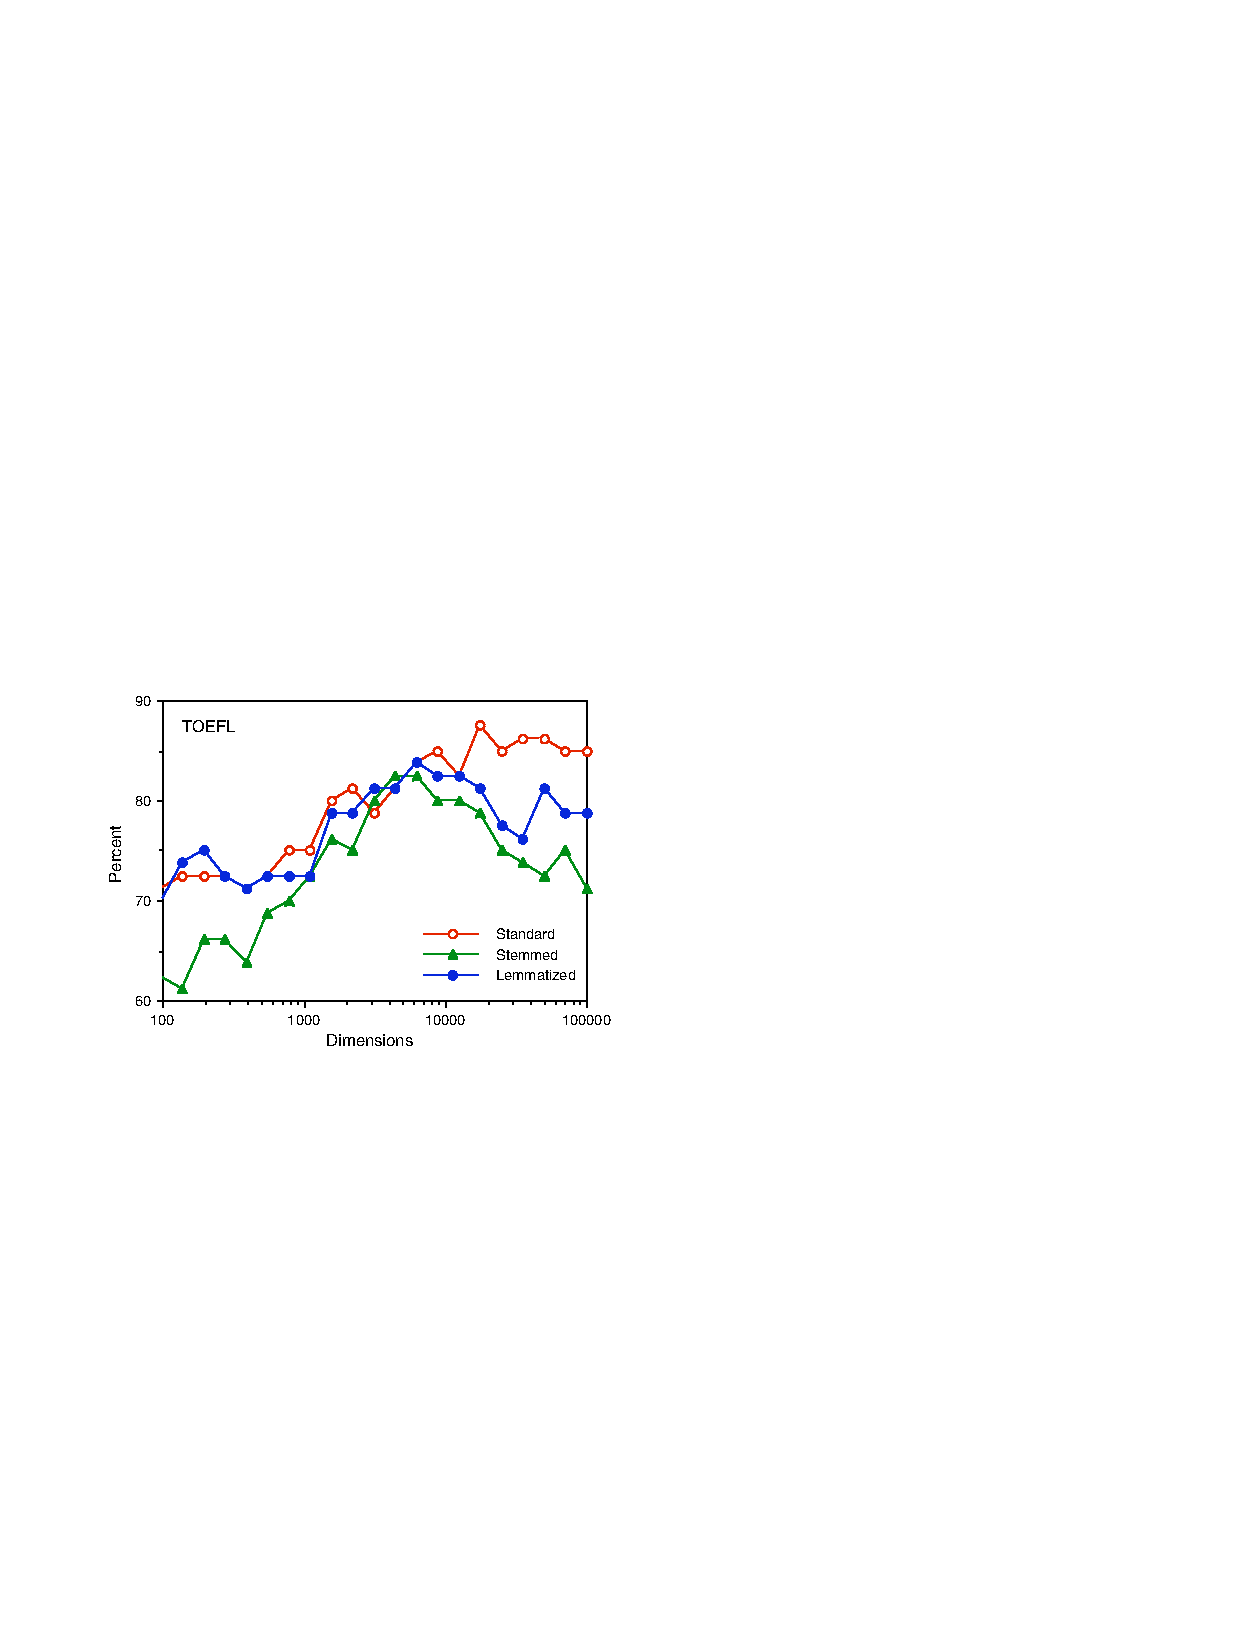
\includegraphics[width=8cm]{img/BullinariaLevy2012_p895_fig4_TOEFL_dim_stem}
  \end{center}

  \ungap[.5]
  \secondary{\scriptsize
    ukWaC corpus. L+R context of size 1. Other parameters presumably as above.
    \par%
  }
\end{frame}

\begin{frame}
  \frametitle{TOEFL results: dimensionality reduction}
  \framesubtitle{\citep[p.~898, Fig.~5]{Bullinaria:Levy:12}}

  \ungap[1]
  \begin{center}
    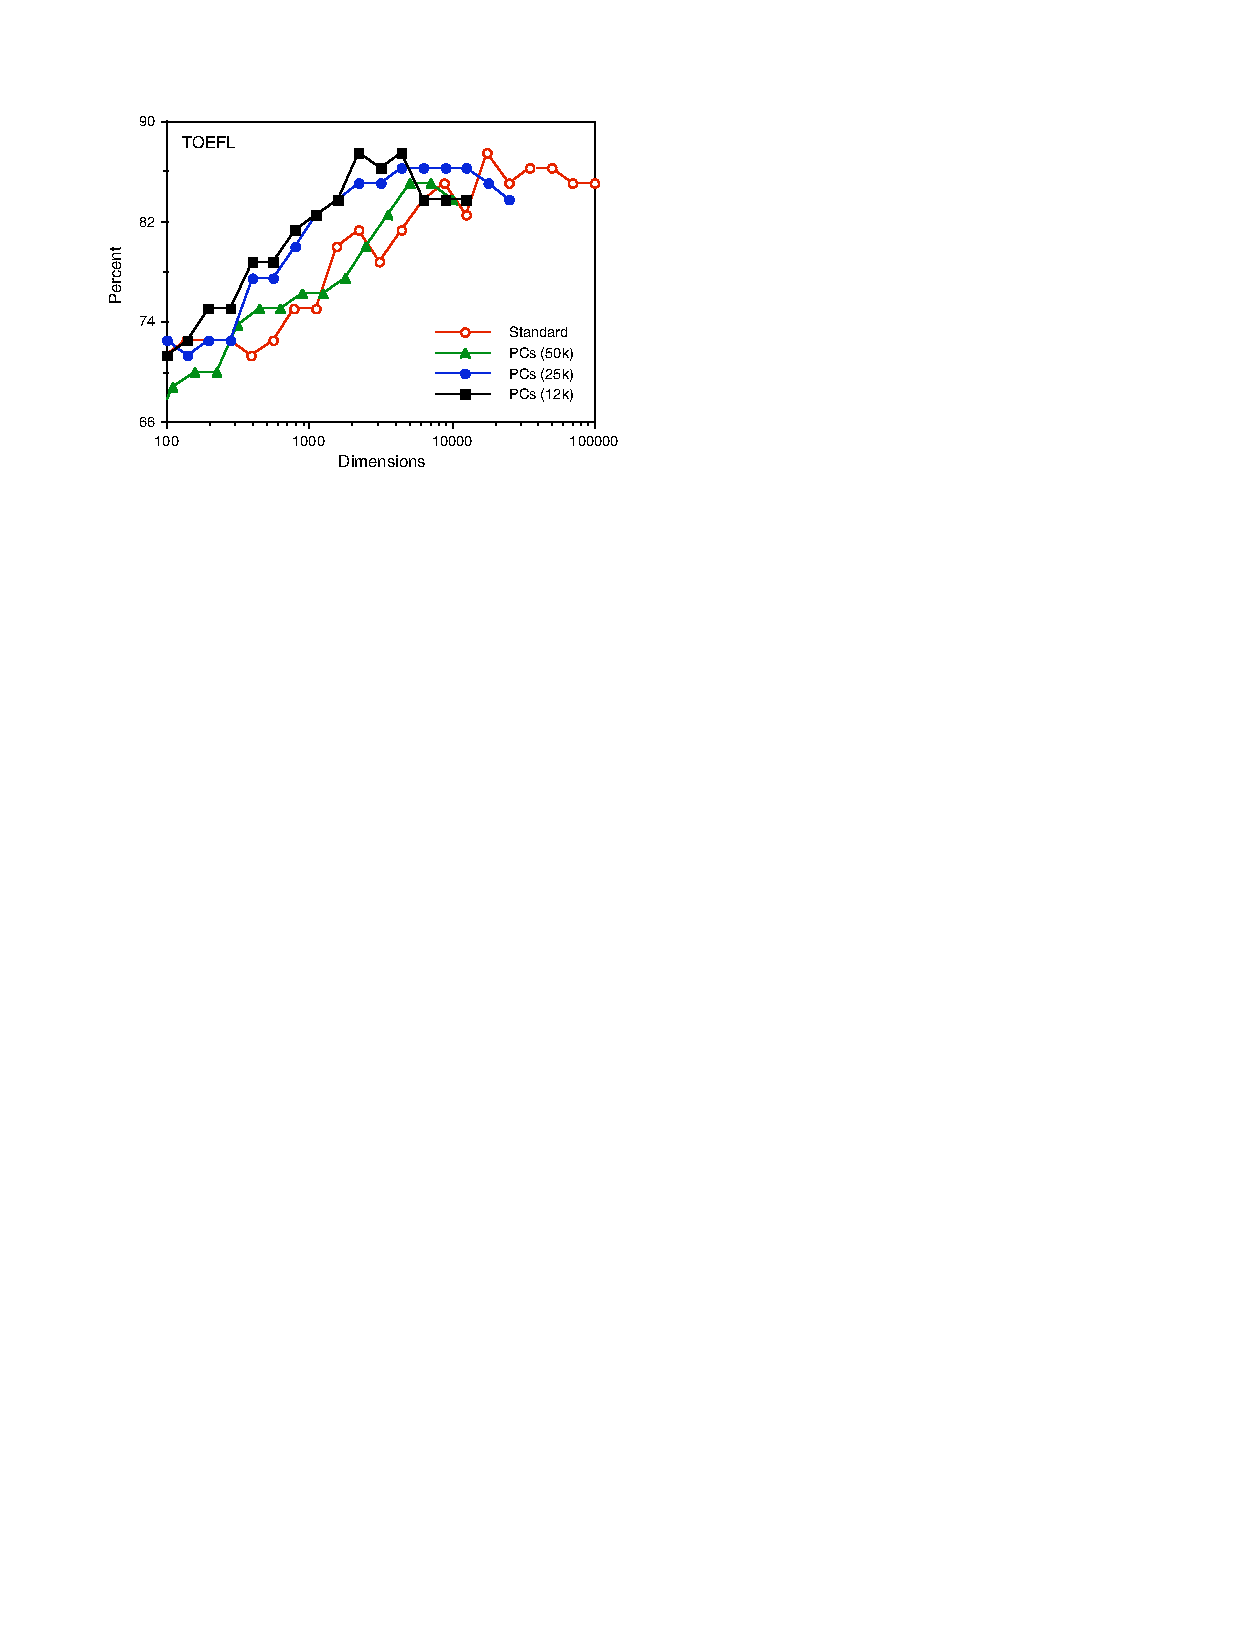
\includegraphics[width=8cm]{img/BullinariaLevy2012_p898_fig5_TOEFL_reddim}
  \end{center}

  \ungap[.5]
  \secondary{\scriptsize
    ukWaC corpus. Positive PMI + cosine. Standard = no dimensionality reduction.
    Other: number of latent dimensions for 12k, 25k and 50k original feature dimensions.
    \par%
  }
\end{frame}

\begin{frame}
  \frametitle{Semantic categorisation: dimensionality reduction}
  \framesubtitle{\citep[p.~898, Fig.~5]{Bullinaria:Levy:12}}

  \ungap[1]
  \begin{center}
    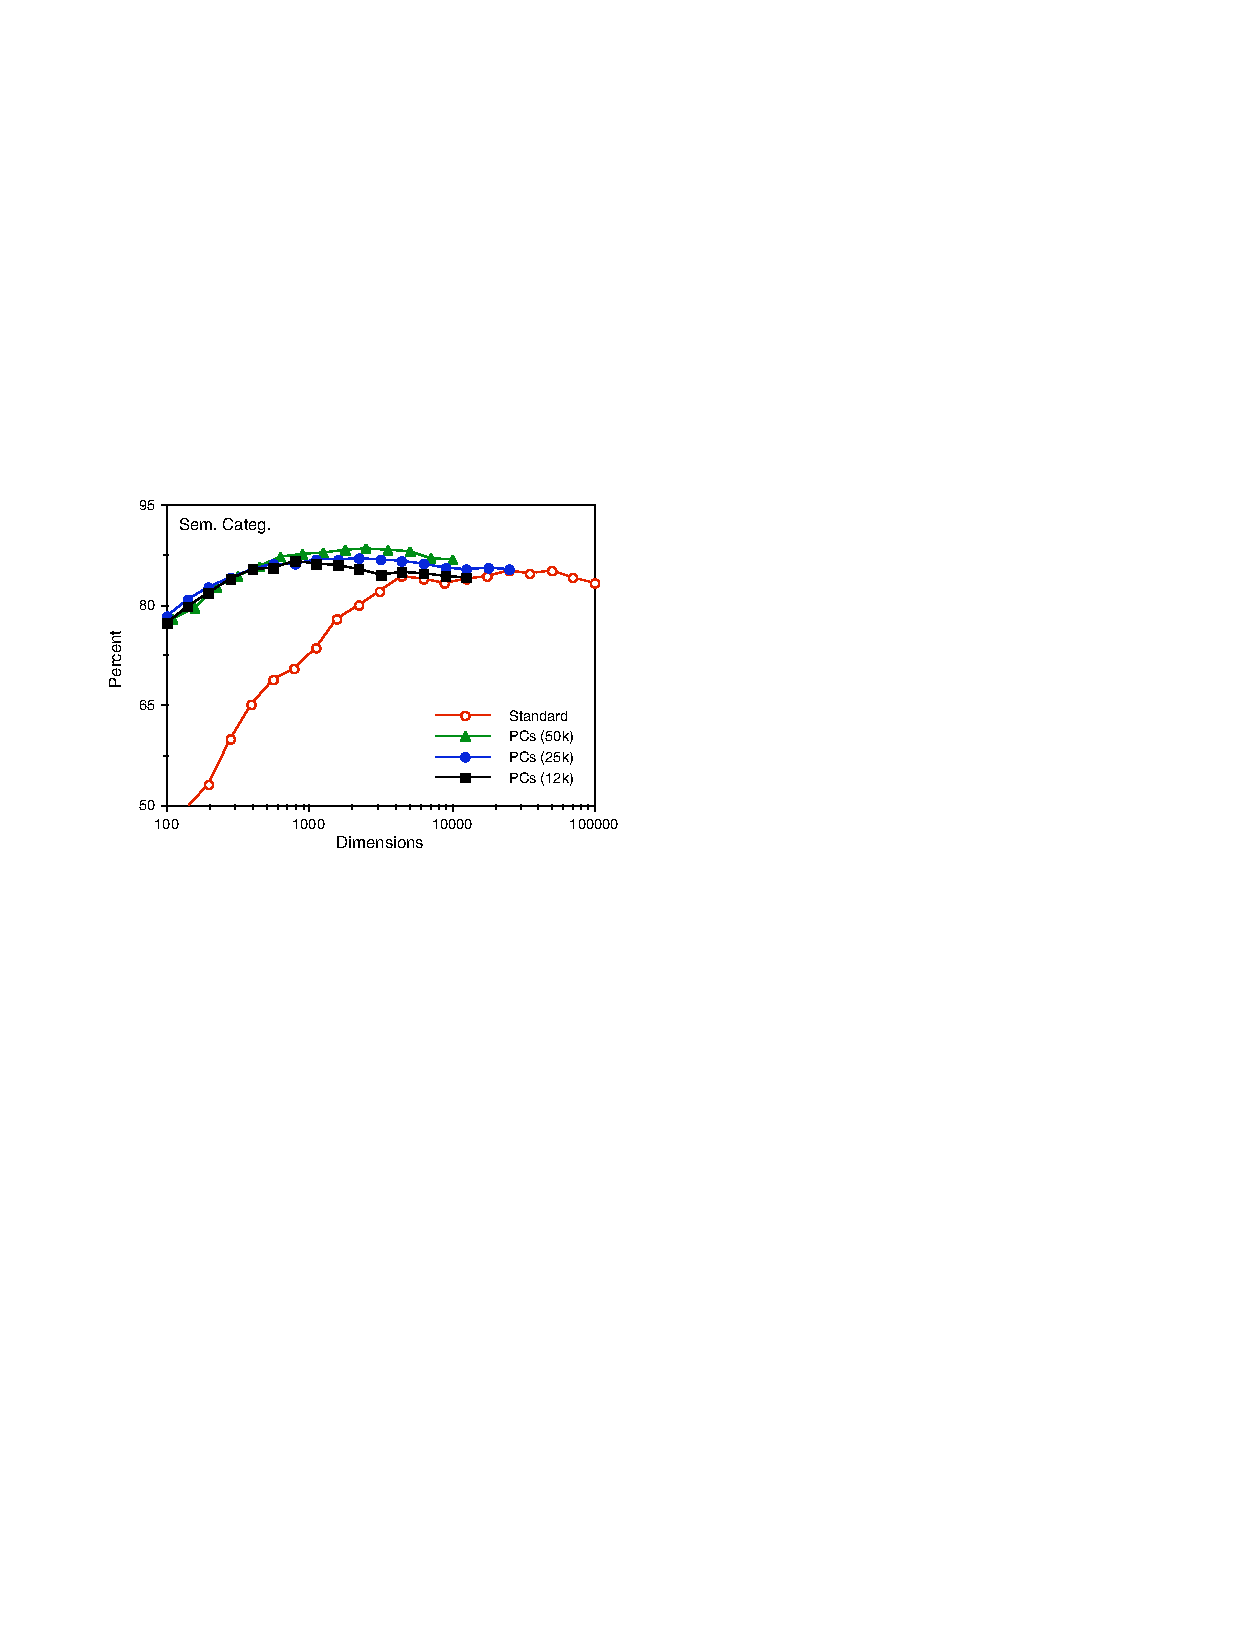
\includegraphics[width=8cm]{img/BullinariaLevy2012_p898_fig5_SemCat_reddim}
  \end{center}

  \ungap[.5]
  \secondary{\scriptsize
    ukWaC corpus. Positive PMI + cosine. Standard = no dimensionality reduction.
    Other: number of latent dimensions for 12k, 25k and 50k original feature dimensions.
    \par%
  }
\end{frame}

\begin{frame}
  \frametitle{Combined results: skipping first latent dimensions}
  \framesubtitle{\citep[p.~900, Fig.~7]{Bullinaria:Levy:12}}

  \ungap[1.5]
  \begin{center}
    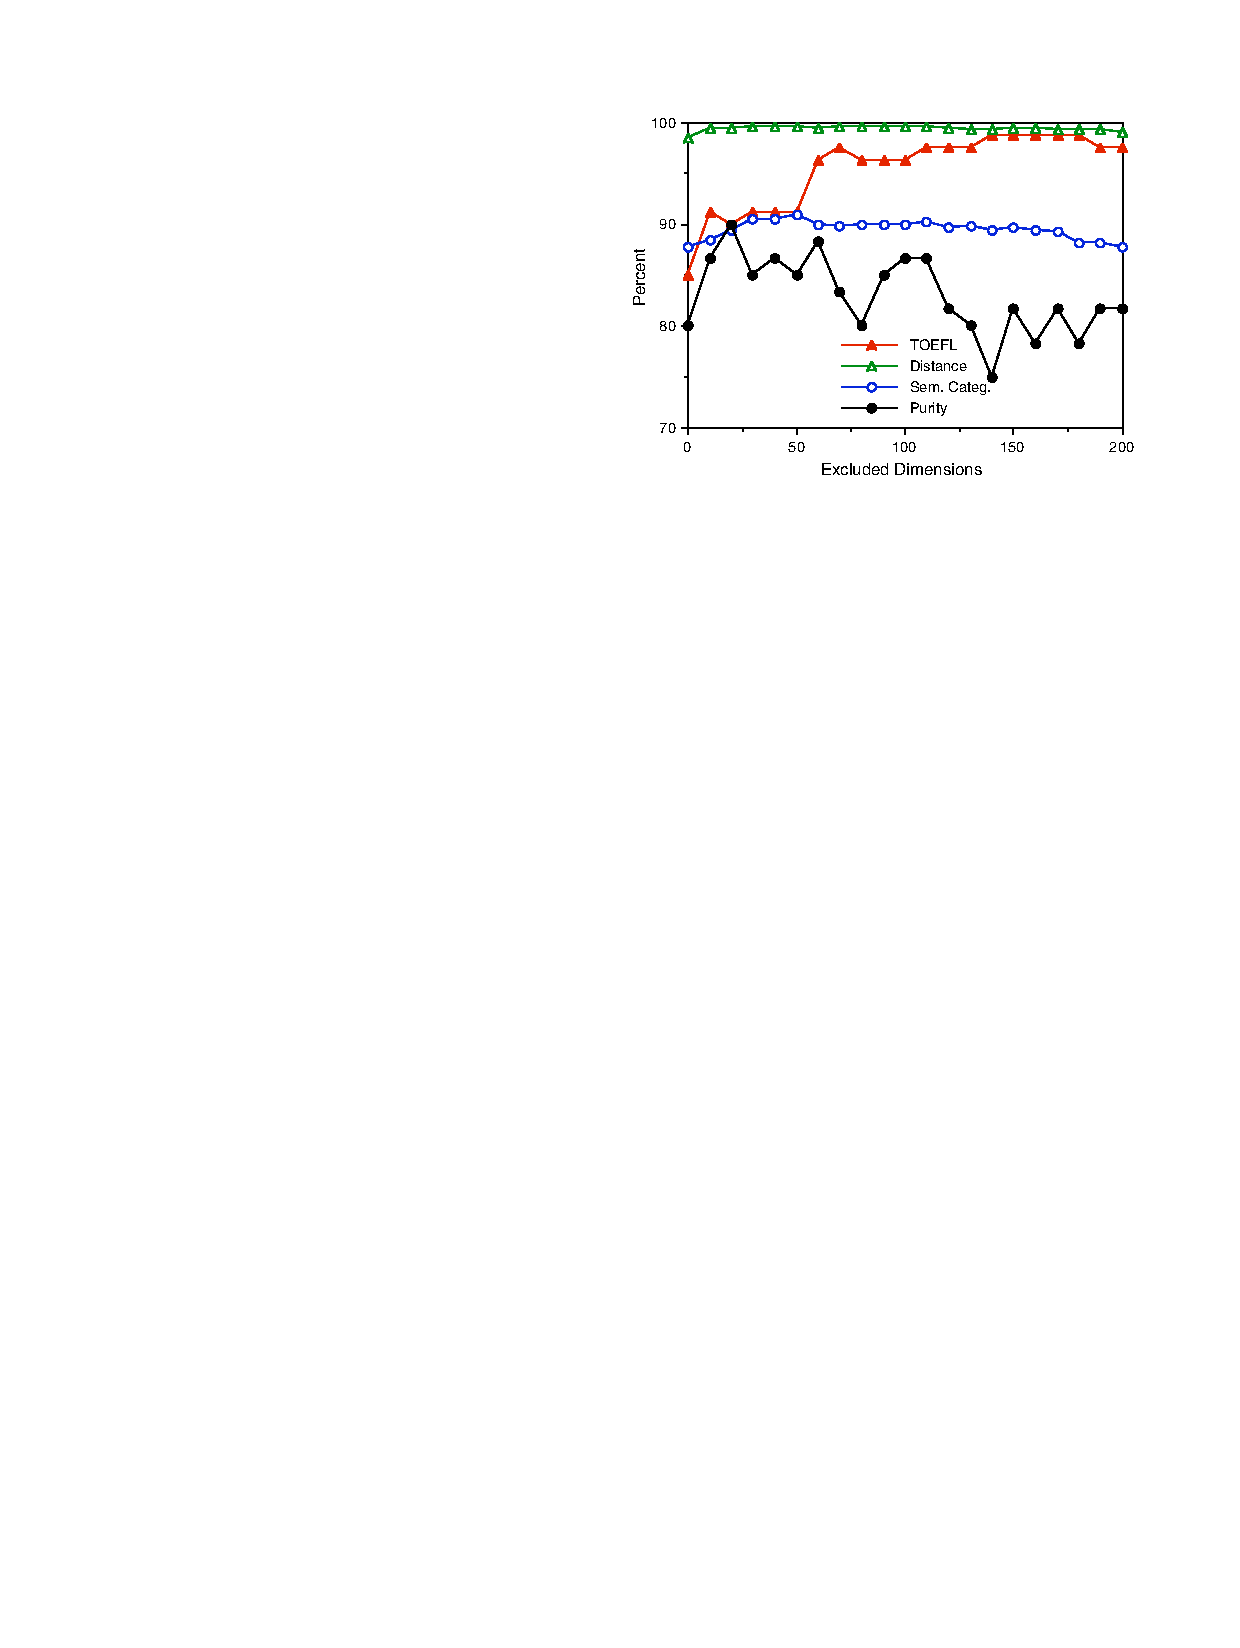
\includegraphics[width=8cm]{img/BullinariaLevy2012_p900_fig7_skipdim}
  \end{center}

  \ungap[.5]
  \secondary{\scriptsize
    ukWaC corpus with standard settings. 50k feature dimensions reduced to 5000 latent dimensions.
    \par%
  }
\end{frame}

\begin{frame}
  \frametitle{TOEFL results: power scaling (Caron's $P$)}
  \framesubtitle{\citep[p.~900, Fig.~7]{Bullinaria:Levy:12}}

  \ungap[1.5]
  \begin{center}
    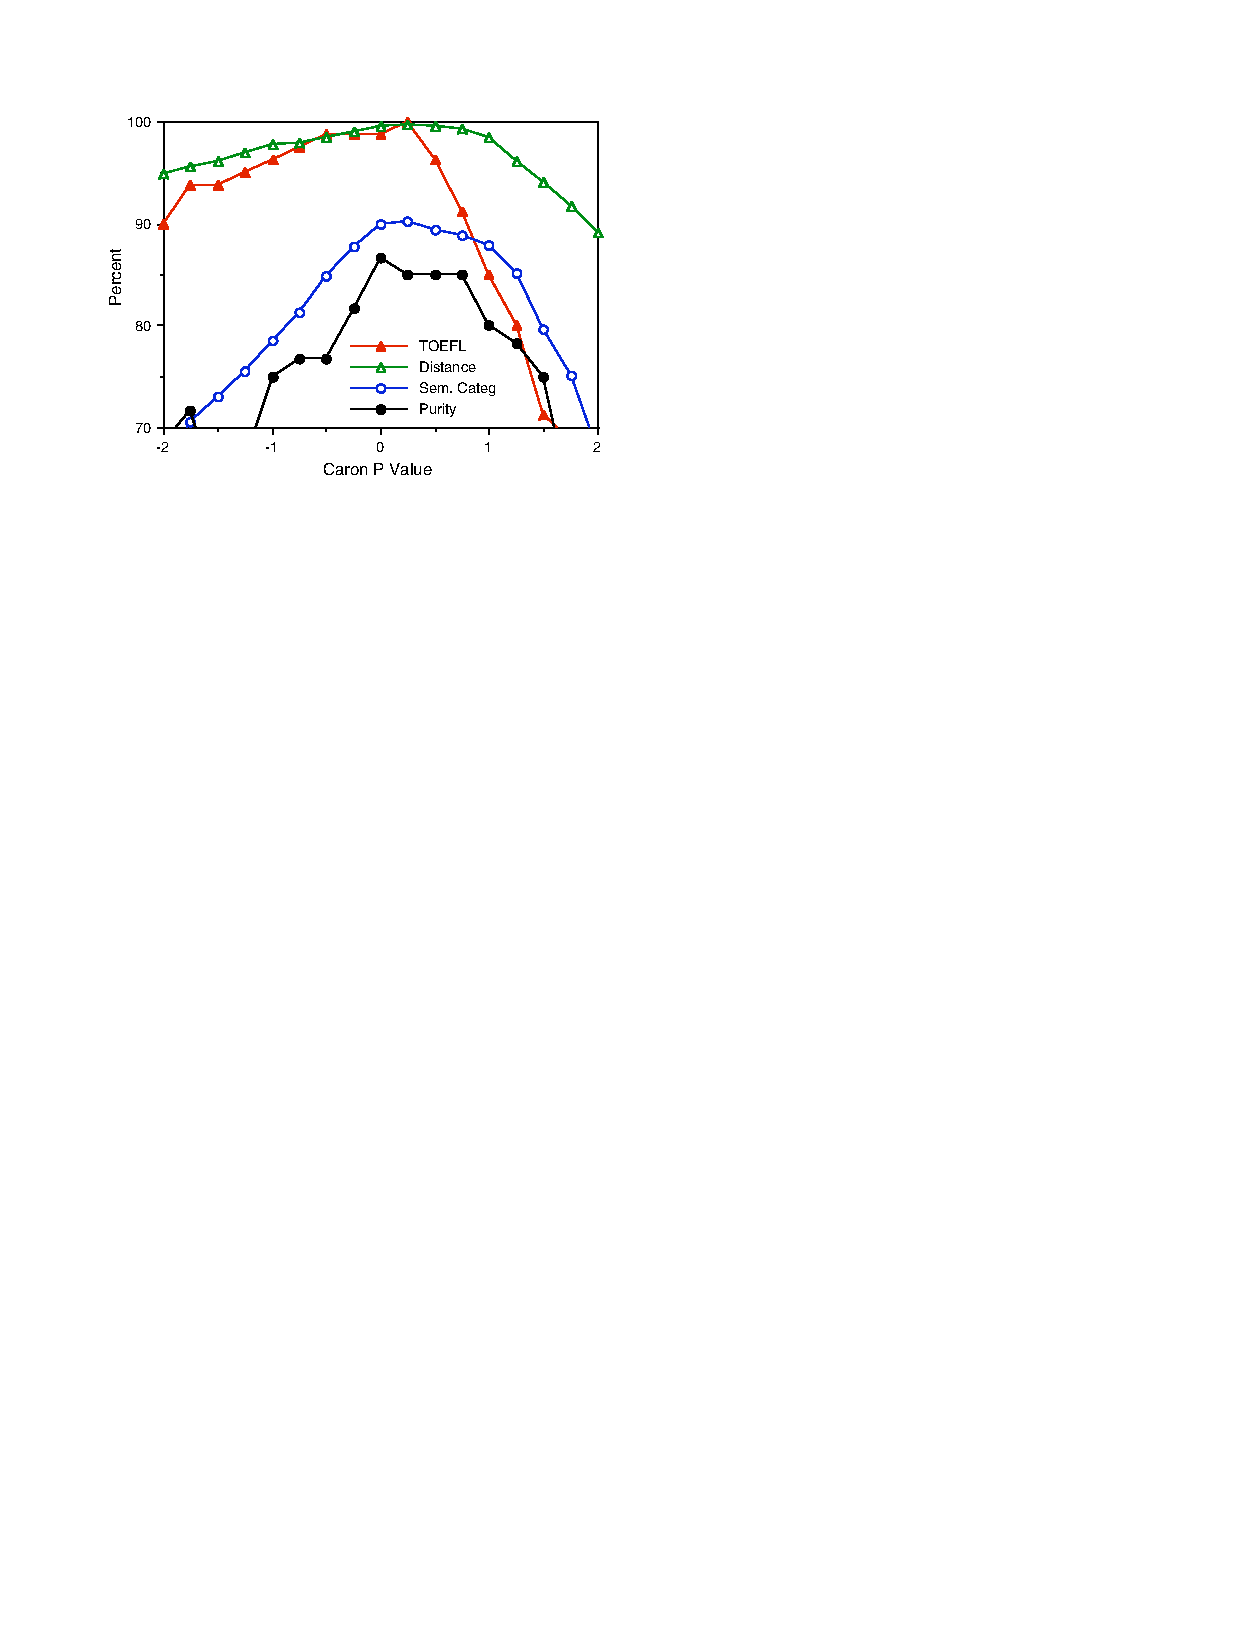
\includegraphics[width=8cm]{img/BullinariaLevy2012_p900_fig7_power}
  \end{center}

  \ungap[.5]
  \secondary{\scriptsize
    ukWaC corpus with standard settings. 50k feature dimensions reduced to 5000 latent dimensions.
    Neutral value is $P = 1$.
    \par%
  }
\end{frame}


%%%%%%%%%%%%%%%%%%%%%%%%%%%%%%%%%%%%%%%%%%
\subsection{Interpreting DSM performance with linear regression}

\begin{frame}
  \frametitle{Making sense of evaluation results}
  \framesubtitle{Interpreting performance \vs picking the best run}
  
  \begin{enumerate}
  \item \hh{One model, many tasks} \citep{Pado:Lapata:07,Baroni:Lenci:10,Pennington:Socher:Manning:14}
    \begin{itemize}
    \item Novel DSM, one (or very few) settings tested on many tasks
    \item Problem: not suitable for the exploration of a large parameter set, very limited coverage of interactions
    \item[]
    \end{itemize}
  \item \hh{Incremental tuning} \citep{Bullinaria:Levy:07,Bullinaria:Levy:12,Kiela:Clark:14,Polajnar:Clark:14}
    \begin{itemize}
    \item Set parameter $a$, then $b$, then $c$
    \item Problem: order dependent, little coverage of interactions
    \item[]
    \end{itemize}
  \item \h{Test all combinations} \citep{Baroni:Dinu:Kruszewski:14,Levy:Goldberg:Dagan:15,Lapesa:Evert:14a}
    \begin{itemize}
    \item Many tasks, many parameters, all combinations
    \item Problem: many runs, \primary{interpreting results is a challenge}
    \end{itemize}
  \end{enumerate}	
\end{frame}

\begin{frame}
  \frametitle{Lots of variation to make sense of... }
  \framesubtitle{TOEFL: 504,000 (!!!) runs \citep{Lapesa:Evert:14a}}

  \ungap[1]
  \begin{center}
    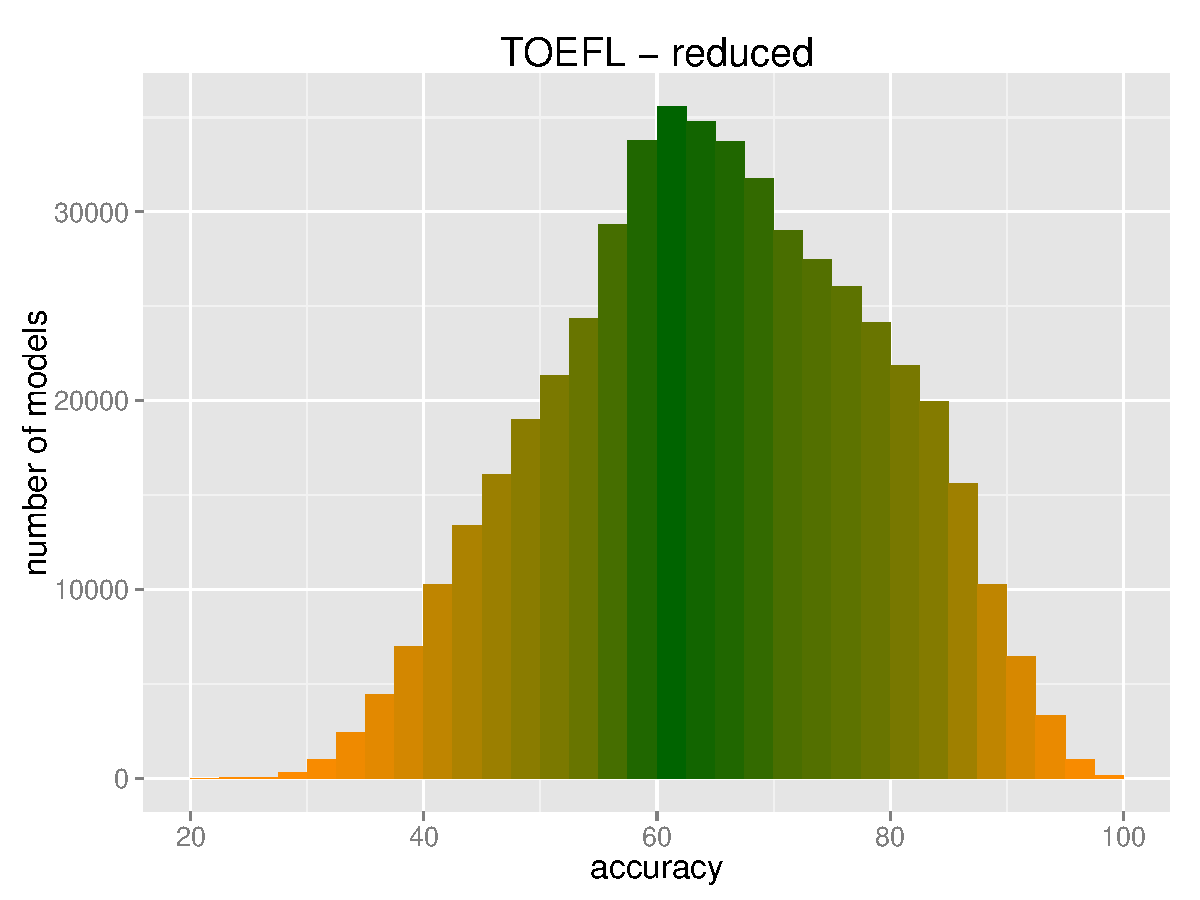
\includegraphics[scale=0.30]{img/lapesa_hist_toefl_reduced}
  \end{center}
  
  \begin{exampleblock}{We need an interpretation methodology that:}
    \begin{itemize}
    \item \ldots{} is able to identify robust trends, avoiding overfitting
    \item \ldots{} is able to capture parameter interactions
    \end{itemize}	
  \end{exampleblock}	
\end{frame}

\begin{frame}
  \frametitle{Linear regression to the rescue}

  \begin{itemize}
  \item Attempts to predict the values of a ``dependent'' variable from one or more ``independent'' variables and their combinations
  \item Is used to understand \secondary{which independent variables are closely related to the dependent variable}, and to \secondary{explore the forms of these relationships}
  \item[]
  \end{itemize}

  \begin{block}{Example}
    \textbf{Dependent variable}: income \\
    \textbf{Independent variables}: gender, age, ethnicity, education level, first letter of the surname \light{(hopefully not significant)}
  \end{block}
\end{frame}
 
\begin{frame}
  \frametitle{How to interpret the evaluation results?}
  \framesubtitle{Our proposal: linear regression}

  We use linear models to analyze the influence of different DSM parameters and their combinations on DSM performance
  \begin{itemize}
  \item dependent variable = \primary{performance}\\
    (accuracy, correlation coefficient, purity)
  \item independent variables = model \primary{parameters}\\
    (e.g.\ source corpus, window size, association score)
  \item[]
  \end{itemize}
  
  \begin{block}{Motivation}
    We want to understand which of the parameters are related to the dependent variable, i.e.\ we want to find the parameters whose manipulation has the strongest effect on DSM performance.
  \end{block}
\end{frame}
 
\begin{frame}
  \frametitle{\Large{How to interpret the evaluation results?}}
  \framesubtitle{Our proposal: linear regression}

  \begin{center}
    \fbox{
      model performance = 
      $\beta_{0} + \beta_1(p_1) + \beta_2(p_2) + \beta_3(p_1, p_2) + \ldots  + \epsilon$
    }
  \end{center} 

  \gap
  \begin{enumerate}
  \item<2-> \primary{Adjusted $R^2$}: proportion of variance explained by the model
    \begin{itemize}
    \item[$\leadsto$] How well do we predict performance?
    \item[]
    \end{itemize}
  \item<3-> \primary{Feature ablation}: proportion of variance explained by a parameter together with all its interactions 
    \begin{itemize}
    \item[$\leadsto$] Which parameters affect performance the most?
    \item[]
    \end{itemize}
  \item<4-> \primary{Model predictions}: visualisation of predicted performance  
    \begin{itemize}
    \item[$\leadsto$] What are the best parameter values?
    \end{itemize}
  \end{enumerate}
\end{frame}   

\begin{frame}<beamer:1| handout:0>
 \frametitle{How well do we predict performance?}
 \framesubtitle{A concrete example: TOEFL, SVD (504k data points)}

 {\small
   \texttt{\textcolor{nicegreen}{accuracy }$\sim$ \ldots{} \phantom{pus + window + score + transformation  \phantom{accuracy $\sim$} + metric + rel.index}}}

 \gap[2]
 \begin{minipage}{1\linewidth}
   \begin{minipage}[c]{0.762\textwidth}
     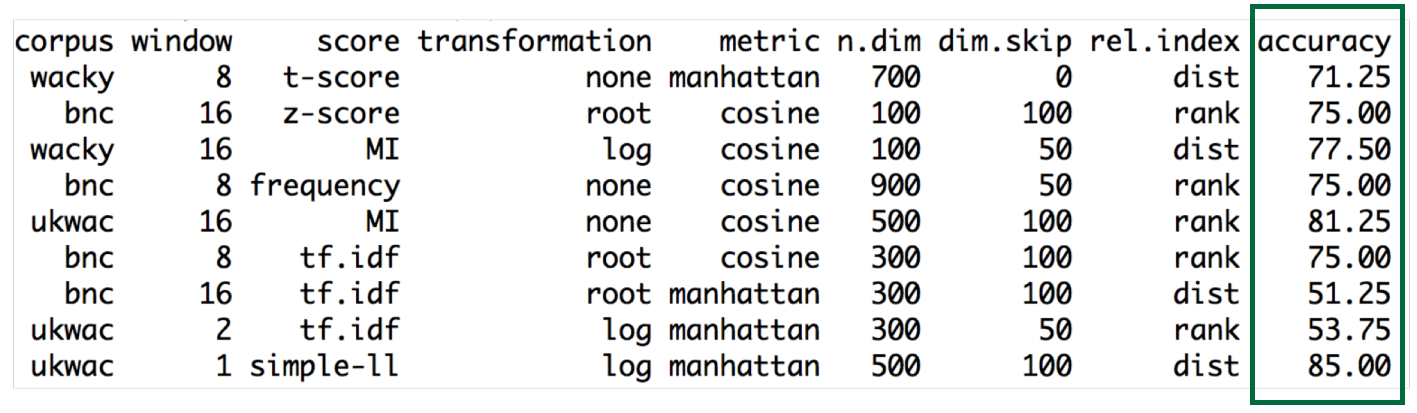
\includegraphics[scale=0.325]{img/dataframeTop123_1}
   \end{minipage}
   \begin{minipage}[c]{0.23\textwidth}
     {\footnotesize\textbf{Model fit: Adj.R$^2$}\\%
       \textcolor{white}{basic \hfill 43\%}\\
       \textcolor{white}{\& SVD \hfill +24\%}\\
       \textcolor{white}{\& 2-way \hfill+22\%}\\
       \textcolor{white}{\& \textit{3-way\hfill+3\%}}}
   \end{minipage}
 \end{minipage} 

 \gap[4]
 \hh{Assumption:} a good linear model acts as a ``smoothing'' algorithm which filters away random noise \& captures robust trends. 
\end{frame}

\begin{frame}<beamer:1| handout:0>
  \frametitle{How well do we predict performance?}
  \framesubtitle{A concrete example: TOEFL, SVD (504k data points)}

  {\small
    \texttt{\textcolor{nicegreen}{accuracy }$\sim$ \textcolor{niceblue}{corpus + window + score + transformation  \phantom{accuracy $\sim$} + metric + rel.index}}}
  
  \gap[2]
  \begin{minipage}{1\linewidth}
    \begin{minipage}[c]{0.762\textwidth}
      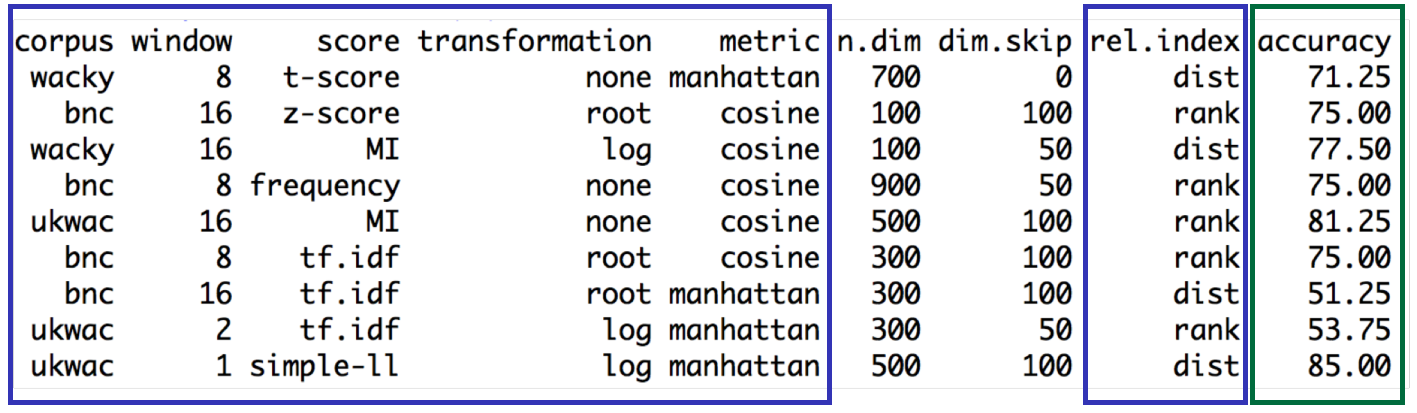
\includegraphics[scale=0.325]{img/dataframeTop123_2}
    \end{minipage}
    \begin{minipage}[c]{0.23\textwidth}
      {\footnotesize\textbf{Model fit: Adj.R$^2$}\\%
        \textcolor{niceblue}{basic} \hfill 43\%\\
        \textcolor{white}{\& SVD \hfill +24\%}\\
        \textcolor{white}{\& 2-way \hfill+22\%}\\
        \textcolor{white}{\& \textit{3-way\hfill+3\%}}}
    \end{minipage}
  \end{minipage} 

  \gap[4]
  \hh{Assumption:} a good linear model acts as a ``smoothing'' algorithm which filters away random noise \& captures robust trends.
\end{frame}
 
\begin{frame}<beamer:1| handout:0>
  \frametitle{How well do we predict performance?}
  \framesubtitle{A concrete example: TOEFL, SVD (504k data points)}

  {\small
    \texttt{\textcolor{nicegreen}{accuracy }$\sim$ \textcolor{niceblue}{corpus + window + score + transformation  \phantom{accuracy $\sim$} + metric + rel.index} \textcolor{nicered}{+ n.dim + dim.skip}}}

  \gap[2]
  \begin{minipage}{1\linewidth}
    \begin{minipage}[c]{0.762\textwidth}
      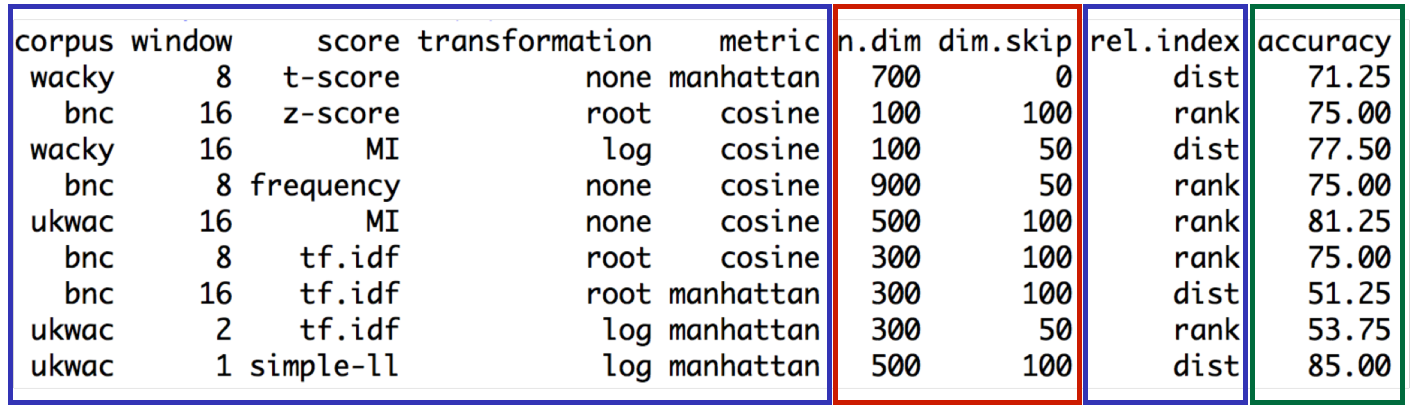
\includegraphics[scale=0.325]{img/dataframeTop123_3}
    \end{minipage}
    \begin{minipage}[c]{0.23\textwidth}
      {\footnotesize\textbf{Model fit: Adj.R$^2$}\\%
        \textcolor{niceblue}{basic} \hfill 43\%\\
        \textcolor{nicered}{\& SVD} \hfill +24\%\\
        \textcolor{white}{\& 2-way \hfill+22\%}\\
        \textcolor{white}{\& \textit{3-way\hfill+3\%}}}
    \end{minipage}
  \end{minipage} 

  \gap[4]  
  \hh{Assumption:} a good linear model acts as a ``smoothing'' algorithm which filters away random noise \& captures robust trends.
\end{frame}
 

\begin{frame}<beamer:1| handout:1>
  \frametitle{How well do we predict performance?}
  \framesubtitle{A concrete example: TOEFL, SVD (504k data points)}

  {\small
    \texttt{\textcolor{nicegreen}{accuracy }$\sim$ \textcolor{niceblue}{corpus * window * score * transformation  \phantom{accuracy $\sim$} * metric * rel.index} \textcolor{nicered}{* n.dim * dim.skip}}}

  \gap[2]
  \begin{minipage}{1\linewidth}
    \begin{minipage}[c]{0.762\textwidth}
      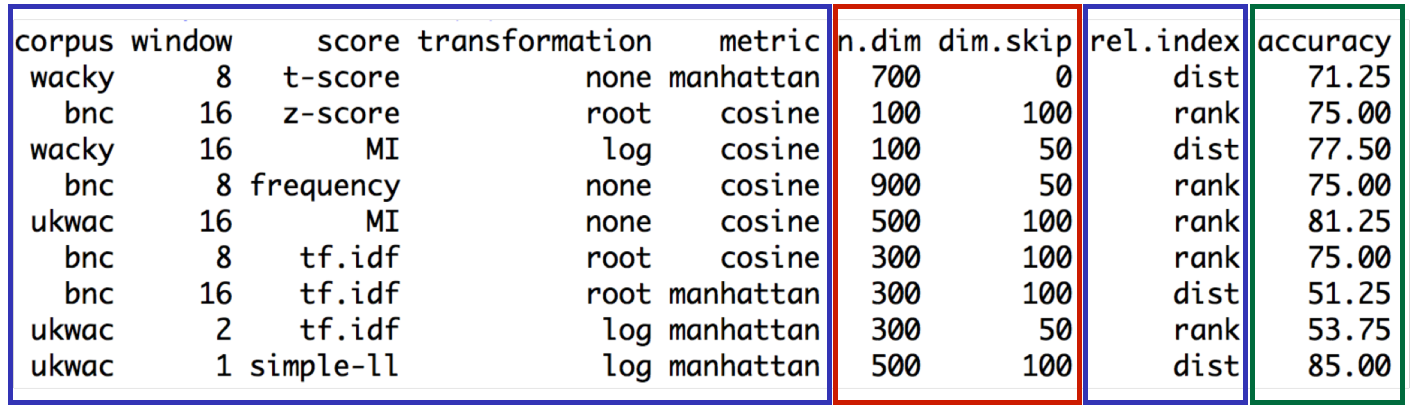
\includegraphics[scale=0.325]{img/dataframeTop123_3}
    \end{minipage}
    \begin{minipage}[c]{0.23\textwidth}
      {\footnotesize\textbf{Model fit: Adj.R$^2$}\\%
        \textcolor{niceblue}{basic} \hfill 43\%\\
        \textcolor{nicered}{\& SVD} \hfill +24\%\\
        \& 2-way \hfill+22\%\\
        \textbf{Total:  \hfill 87\%}}
    \end{minipage}
  \end{minipage} 

  \gap[4]
  \hh{Assumption:} a good linear model acts as a ``smoothing'' algorithm which filters away random noise \& captures robust trends.
\end{frame}
 
\begin{frame}
  \frametitle{Which parameters affect performance the most?}
  \framesubtitle{Feature ablation: parameters and interactions on TOEFL}
  
  \begin{columns}    
    \begin{column}{0.5\textwidth}
      \vspace*{-10pt}
      \begin{figure} 
        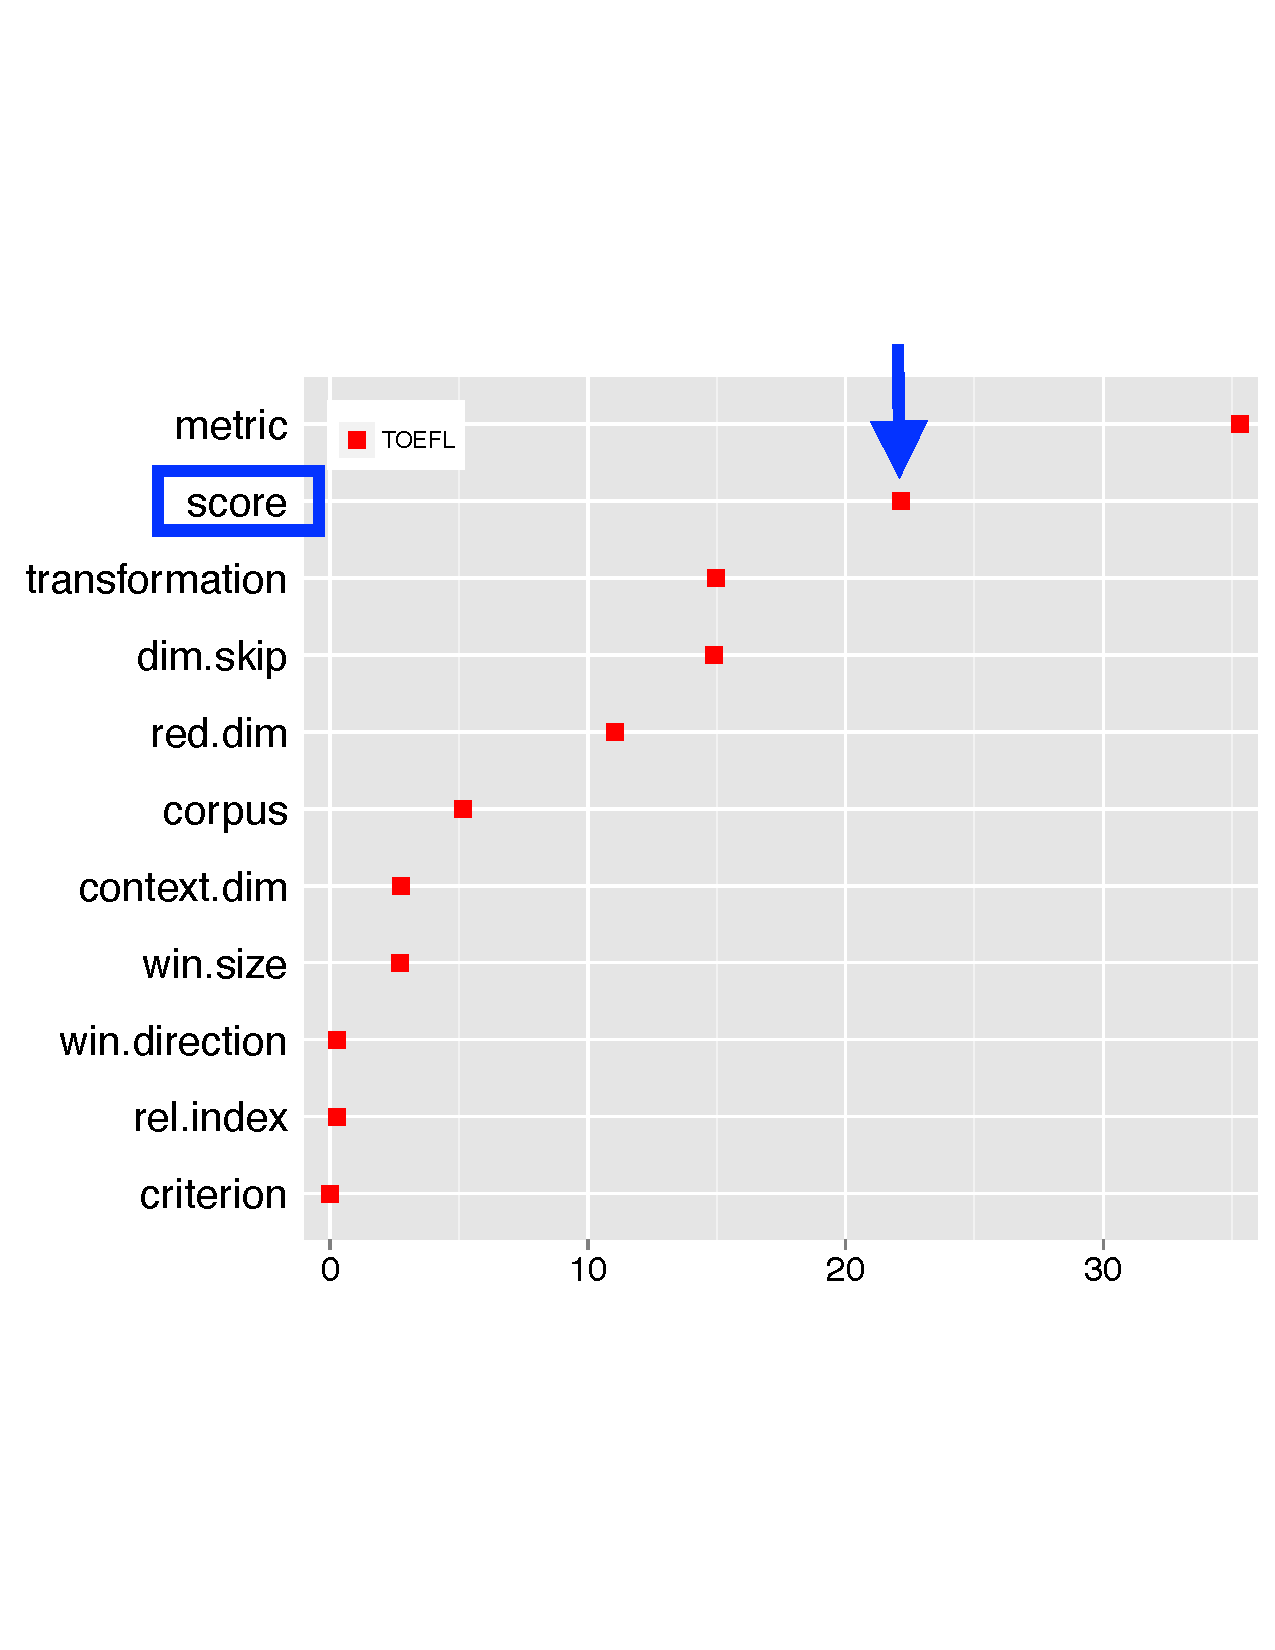
\includegraphics[scale=0.30]{img/toefl_reduced_main_r2_ann}
        \vspace{-10pt}
      \end{figure}
    \end{column}     

    \begin{column}{0.5\textwidth}
      \begin{table}\footnotesize
        \vspace*{18pt}
        \begin{tabular}{lrrrr} 
          \textbf{Effect} & \textbf{$R^2$}  \\ \hline
          score & 10.53 \\
          \hline
          score:transformation & 7.42 \\   
          score:metric & 1.77 \\ 
          corpus:score & 0.84 \\  
          score:context.dim & 0.64 \\  \hline
          other int. $<$ 0.5  & 0.93  \\ \hline
          \textbf{Feature ablation} & \h{22.13} \\
        \end{tabular}
        \vspace{5pt}
      \end{table}
    \end{column}
  \end{columns}  
 \end{frame}

 \begin{frame}
   \frametitle{Which parameters affect performance the most?}
   \framesubtitle{Interaction of score and transformation: effect plot}
   \centering
   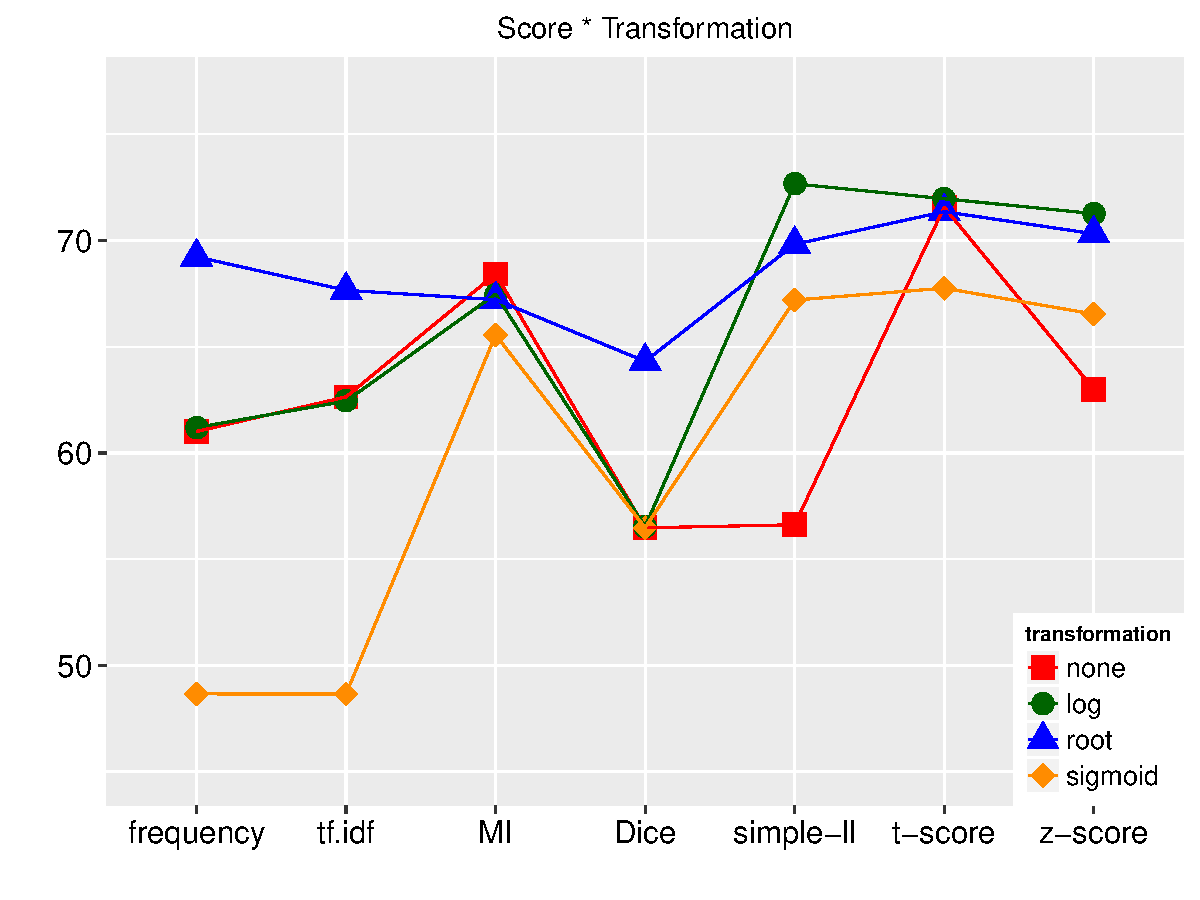
\includegraphics[scale=0.45]{img/toefl-bow_reduced_main_score_transformation}
 \end{frame}

 \begin{frame}
   \frametitle{So, are there general trends? \citep{Lapesa:Evert:14a}}
   \framesubtitle{Datasets: TOEFL, RG65, WordSim353, ESSLLI08 (and 3 other clust. datasets)}

   \begin{itemize}
   \item<2-> Most explanatory parameters: similar across tasks/datasets
     \begin{itemize}
     \item simple-ll + logarithmic transformation, cosine similarity
     \item[]
     \end{itemize}
   \item<3-> Parameters that show variation: \primary{the amount and nature} of shared context
     \begin{itemize}
     \item Context window: 4 is a good compromise solution
     \item SVD: always helps, and skipping the first dimensions (but not too many) generally helps 
     \item[]
     \end{itemize}
   \item<4-> Neighbor rank (almost) always better than distance
     \begin{itemize}
     \item[]
     \end{itemize}
   \item<5-> Syntax (almost) never helps :( \citep{Lapesa:Evert:17}  
   \end{itemize}
 \end{frame}

%%%%%%%%%%%%%%%%%%%%%%%%%%%%%%%%%%%%%%%%%%%%%%%%%%%%%%%%%%%%%%%%%%%%%%
\section{Appendix: A large-scale evaluation study}

\begin{frame}[c]
  \centering

  \textbf{Appendix}\\
  \hh{\large A (very) large-scale evaluation study}
  
  \gap[2]
  \citep{Lapesa:Evert:14a}
\end{frame}

%%%%%%%%%%%%%%%%%%%%%%%%%%%%%%%%%%%%%%%%%%
\subsection{Tasks \& parameters}

\begin{frame}
  \frametitle{Tasks}

  \begin{enumerate}
  \item \hh{Classification}
    \begin{itemize}
    \item \code{TOEFL80}: multiple-choice classification task\\ \citep{Landauer:Dumais:97}
    \item[]
    \end{itemize}
  \item \hh{Correlation to Similarity Ratings}
    \begin{itemize}
    \item \code{RG65}: 65 noun pairs \citep{Rubenstein:Goodenough:65}
    \item \code{WordSim353}: 351 noun pairs \citep{Finkelstein:etc:02}
    \item[]
    \end{itemize}  
  \item \hh{Semantic Clustering} 
    \begin{itemize} 
    \item \code{Battig82}: 82 nouns, 10 classes \citep{VanOverschelde:Rawson:Dunlosky:04}
    \item \code{AP402}: 402 nouns, 21 classes \citep{Almuhareb:06}
    \item \code{ESSLLI08\_Nouns}: 44 nouns, 6 classes
    \item Mitchell: 60 nouns, 12 classes \citep{Mitchell:etc:08}
    \item[]
    \end{itemize}   
  \end{enumerate}
\end{frame}

\begin{frame}
  \frametitle{Distributional models: general features}
  \begin{itemize}
  \item \primary{Term-term} distributional semantic models (bag-of-words)
  \item \secondary{Target} terms (rows)
    \begin{itemize}
    \item vocabulary from Distributional Memory \citep{Baroni:Lenci:10} + terms from evaluation datasets
    \item 27522 lemma types 
    \end{itemize} 
  \item \secondary{Feature} terms (columns)
    \begin{itemize}
    \item filtered by part-of-speech (nouns, verbs, adjectives, adverbs)
    \item further context selection determined by two model parameters
    \end{itemize}
  \end{itemize}

  \begin{block}{}\footnotesize
    Distributional models were compiled and evaluated using the IMS \primary{Corpus Workbench}\footnote{\scriptsize\url{http://cwb.sf.net/}}, the \primary{UCS toolkit}\footnote{\scriptsize\url{http://www.collocations.de/software.html}} and the \primary{\texttt{wordspace} package} for R.
  \end{block}
\end{frame}

\begin{frame}
  \frametitle{Evaluated parameters}
  \framesubtitle{Building the co-occurrence matrix}
  \begin{enumerate}
  \item   \h{Source corpus}: BNC, Wackypedia, UkWac
    \begin{block}{}\small
      Our source corpora -- standard choices in distributional semantics -- differ in both size and quality. Is there a quantity/quality trade-off?
    \end{block}
    
  \item  \textbf{Window} (= surface span)
    \begin{itemize}
    \item  \h{Direction}: directed (= structured), undirected
    \item  \h{Size}: 1, 2, 4, 8, 16 words
    \end{itemize}   
    
    \begin{block}{}\small
      We expect those parameters to be crucial as they determine the granularity (direction) and amount (size) of shared context involved in the computation of similarity.  
    \end{block}          
  \end{enumerate}   
\end{frame}

\begin{frame}
  \frametitle{Evaluated parameters}
  \framesubtitle{Selecting dimensions from the co-occurrence matrix} 
  \begin{enumerate}
    \setcounter{enumi}{2} 
  \item \textbf{Feature selection}: 
    \begin{itemize}
    \item   \h{Criterion}: frequency, number of non-zero entries 
    \item   \h{Threshold}: top $n$ dimensions ($n$ = 5000, 10000, 20000, 50000, 100000)
    \end{itemize}          
    \begin{block}{}\small
      How many context dimensions (words) are needed for DSMs to perform well in specific tasks? Are too many context dimensions detrimental? What is the best selection criterion? 
    \end{block}   
  \end{enumerate}   
\end{frame}


\begin{frame}
  \frametitle{Evaluated parameters}
  \framesubtitle{Weighting and scaling co-occurrence counts} 
  
  \begin{enumerate}
    \setcounter{enumi}{3}
    
  \item   \h{Feature scoring}: frequency, simple-ll, MI, Dice, t-score, z-score, tf.idf
    \begin{block}{}\small
      Association measures represent an interpretation of co-occurrence frequency, and they emphasize different types of collocations \citep{Evert:08}. Does this have an effect on DSM performance? 
    \end{block}
    
  \item  \h{Transformation}: none, logarithmic, square root, sigmoid
    \begin{block}{}\small
      Transformations reduce the skewness of feature scores.
    \end{block}
  \end{enumerate}   
\end{frame}

\begin{frame}
  \frametitle{Evaluated parameters}
  \framesubtitle{Dimensionality reduction}    

  \begin{enumerate}
    \setcounter{enumi}{5}
  \item \textbf{Dimensionality reduction} with randomized SVD:
    \begin{itemize}
    \item \h{number of reduced dimensions}: 100, 300, 500, 700, 900
    \item \h{number of skipped dimensions}: 0, 50, 100
    \end{itemize}    
    \begin{block}{}\small
      Dimensionality reduction is expected to improve semantic representation and make computations more efficient. How does SVD interact with the other parameters?
      \citet{Bullinaria:Levy:12} report improvements in some tasks (e.g.\ TOEFL) when the first latent dimensions (with highest variance) are discarded. Does this result generalize to our tasks/datasets? 
    \end{block}                  
  \end{enumerate}   
\end{frame}

\begin{frame}
  \frametitle{Evaluated parameters}
  \framesubtitle{Computation and usage of distances}   

  \begin{enumerate}
    \setcounter{enumi}{6}      
  \item   \h{Distance metric}: cosine (angular distance), manhattan
    \begin{block}{}\small
      Both are symmetric, while cognitive processes are often asymmetric
    \end{block}
    
  \item  \h{Index of distributional relatedness}
    \begin{itemize}
    \item \textbf{distance}: $\mathop{\text{dist}}(a,b)$
    \item  \textbf{neighbor rank}, calculated differently for different tasks:
      \begin{itemize}
      \item TOEFL: backward rank, i.e.\ $\mathop{\text{rank}}(b,a)$
      \item Ratings and Clustering: average of logarithmic forward and backward rank, i.e.\ $\bigl(\log \mathop{\text{rank}}(a,b) + \log \mathop{\text{rank}}(b,a)\bigr) / 2$
      \end{itemize}
    \end{itemize}    
    \begin{block}{}\small
      This parameter allows us to account for asymmetries: $\mathop{\text{rank}}(b,a)$ is different from $\mathop{\text{rank}}(a,b)$. While cognitively plausible, neighbor rank is computationally expensive: does it improve the performance of DSMs?
    \end{block}                
    
  \end{enumerate}   
\end{frame}

%%%%%%%%%%%%%%%%%%%%%%%%%%%%%%%%%%%%%%%%%%
\subsection{Evaluation results}

\begin{frame}
  \frametitle{TOEFL multiple-choice classification task}
  \framesubtitle{Introducing the task}

  A collection of 80 multiple-choice questions from a synonym task in the Test Of English as a Foreign Language (TOEFL) 
  \begin{exampleblock}{TOEFL dataset}
    Target: \secondary{\emph{consume}} -- Choices: \emph{breed, catch, \primary{eat}, supply} \\
    Target: \secondary{\emph{constant}} -- Choices:  \emph{accidental, \primary{continuing}, instant, rapid}  \\
    Target: \secondary{\emph{concise}}\hspace{1ex} -- Choices: \emph{free, positive, powerful, \primary{succinct}} \\
  \end{exampleblock}
  \begin{itemize}
  \item A \textbf{classification} task
  \item If DSMs capture synonymy relations, we expect that \primary{the distance between the target and the correct choice will be smaller than to the wrong choices}
  \item Performance: \textbf{\% accuracy}
  \end{itemize}

  
\end{frame}

\begin{frame}
  \frametitle{TOEFL task: performance}
  \framesubtitle{Unreduced versus Reduced Experiments}
  \centering
  
  \begin{columns}

    \begin{column}{0.5\textwidth}
      \centering
      \hspace*{-18pt}   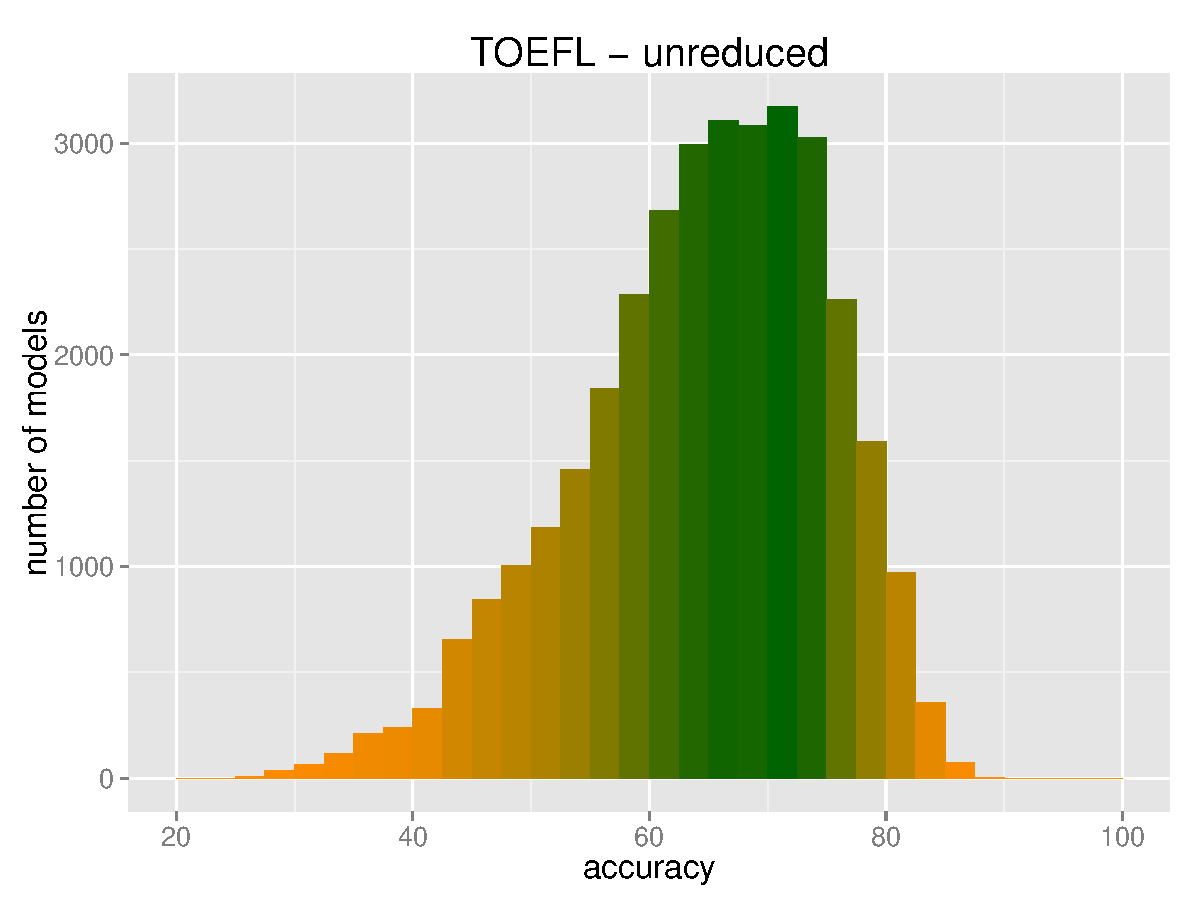
\includegraphics[scale=0.30]{img/lapesa_hist_toefl_unreduced}
      \begin{block}{}\footnotesize \centering
        Min:  25 ; Max: 87.5 ;  Mean: 63.9
      \end{block}
    \end{column}
    \begin{column}{0.5\textwidth}
      \hspace*{-18pt} 
      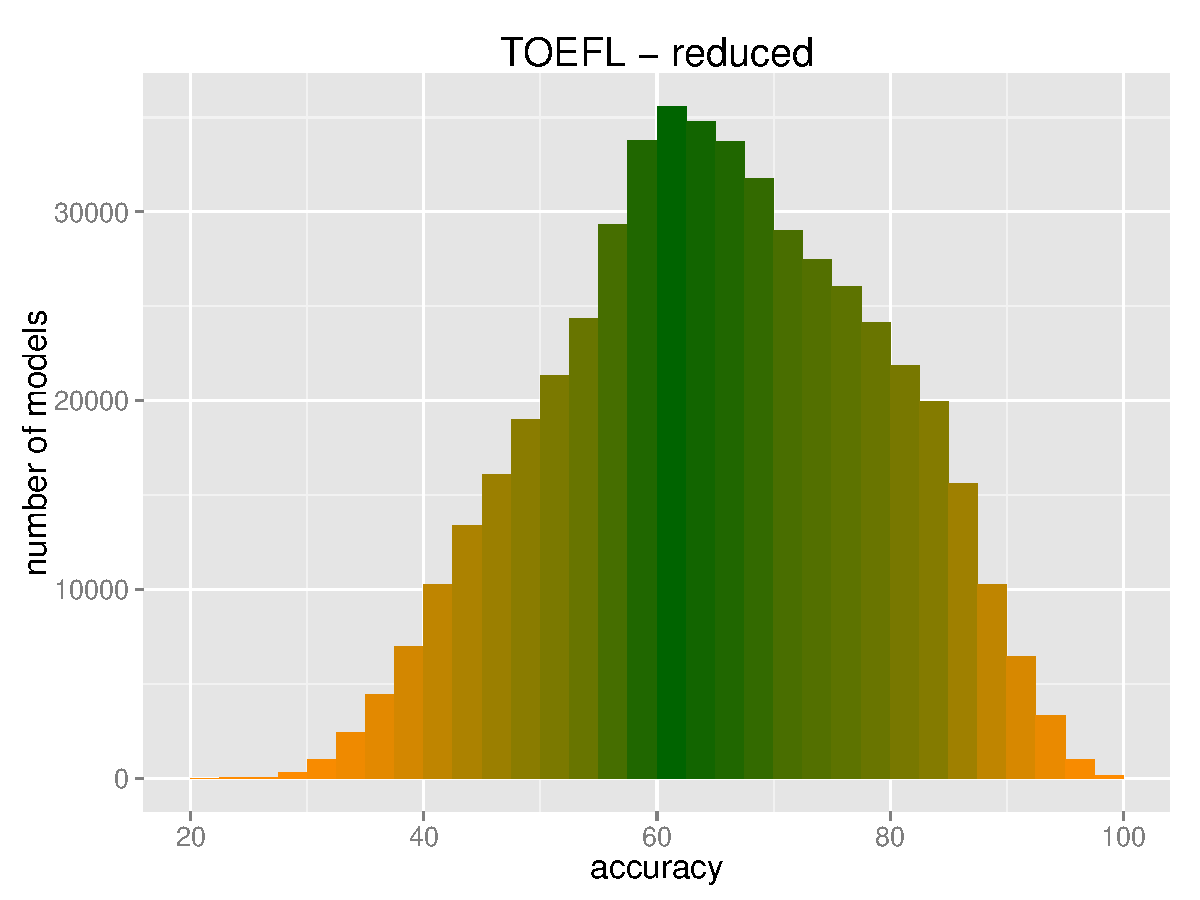
\includegraphics[scale=0.30]{img/lapesa_hist_toefl_reduced}
      \begin{block}{}\footnotesize \centering
        Min:  18.7; Max: \primary{97.4};  Mean: 64.4
      \end{block}
    \end{column}
  \end{columns}
\end{frame}

\begin{frame}
  \frametitle{TOEFL task: parameters and explained variance}
  \framesubtitle{Reduced setting: feature Ablation  (model $R^{2}$: 89\%)}
  \centering
  \hspace*{-10pt}
  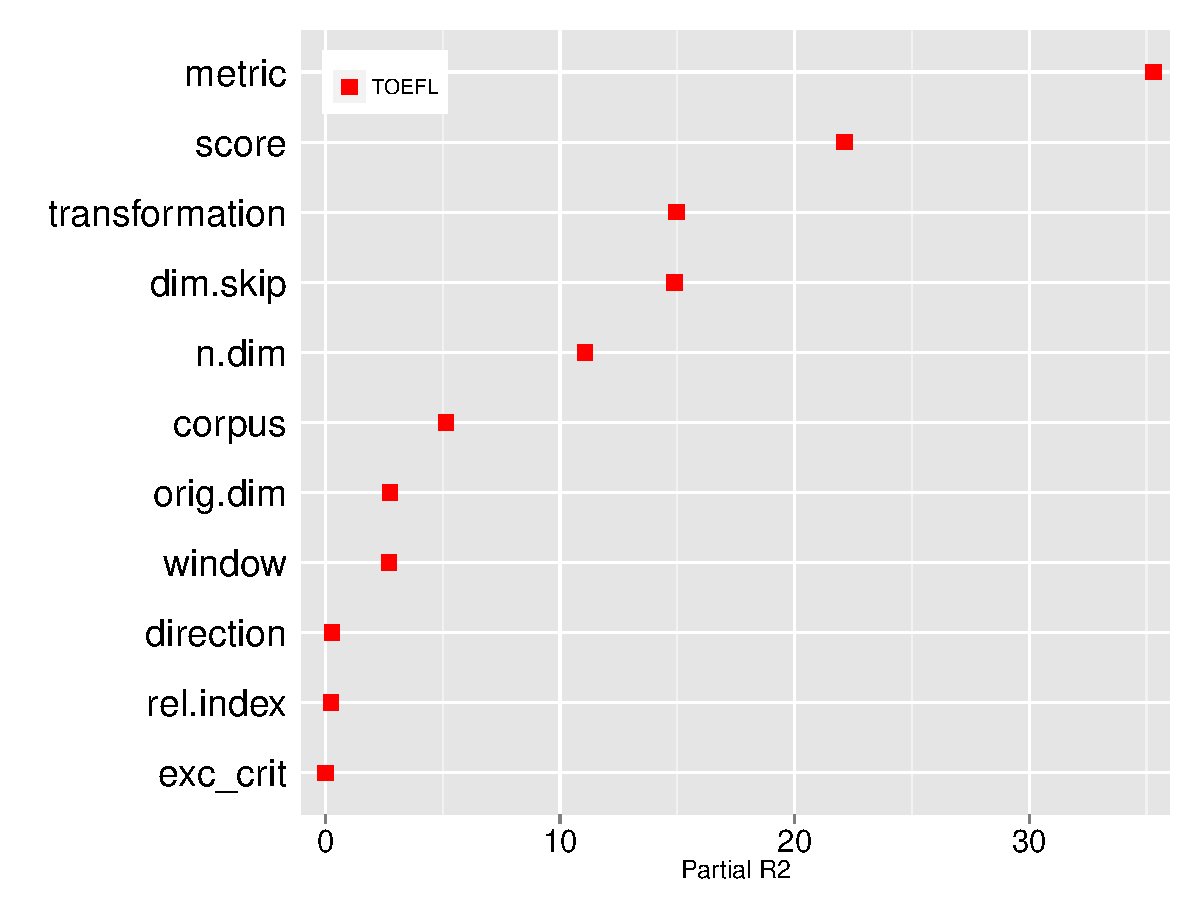
\includegraphics[scale=0.45]{img/lapesa_toefl_main_r2_reduced}

\end{frame}

\begin{frame}
  \frametitle{TOEFL task: interactions}
  \framesubtitle{Reduced setting ($R^{2}$ $>$ 0.5)}

  \begin{center}
    \begin{tabular}{lrrrr}
      Interaction & Df &  R$^2$  \\ \hline
      \primary{score:transformation} & 18  & 7.42 \\   
      \primary{metric:dim.skip} & 2  & 4.44 \\ 
      \primary{score:metric} & 6  & 1.77 \\ 
      metric:orig.dim & 4  & 0.98 \\ 
      window:transformation & 12  & 0.91 \\     
      corpus:score & 12  & 0.84 \\  
      score:orig.dim & 24  & 0.64  \\ 
      metric:n.dim & 4  & 0.63  \\ 
    \end{tabular}

    \gap[1]
    \secondary{TOEFL task: interactions, $R^2$}
  \end{center}  
\end{frame}

\begin{frame}
  \frametitle{TOEFL task: Metric, Score, Transformation}
  \framesubtitle{Partial effect displays \citep{Fox:03}} 

  \centering
  \only<beamer:1-2| handout:0>{\ungap[1]}%
  \only<beamer:1| handout:0>{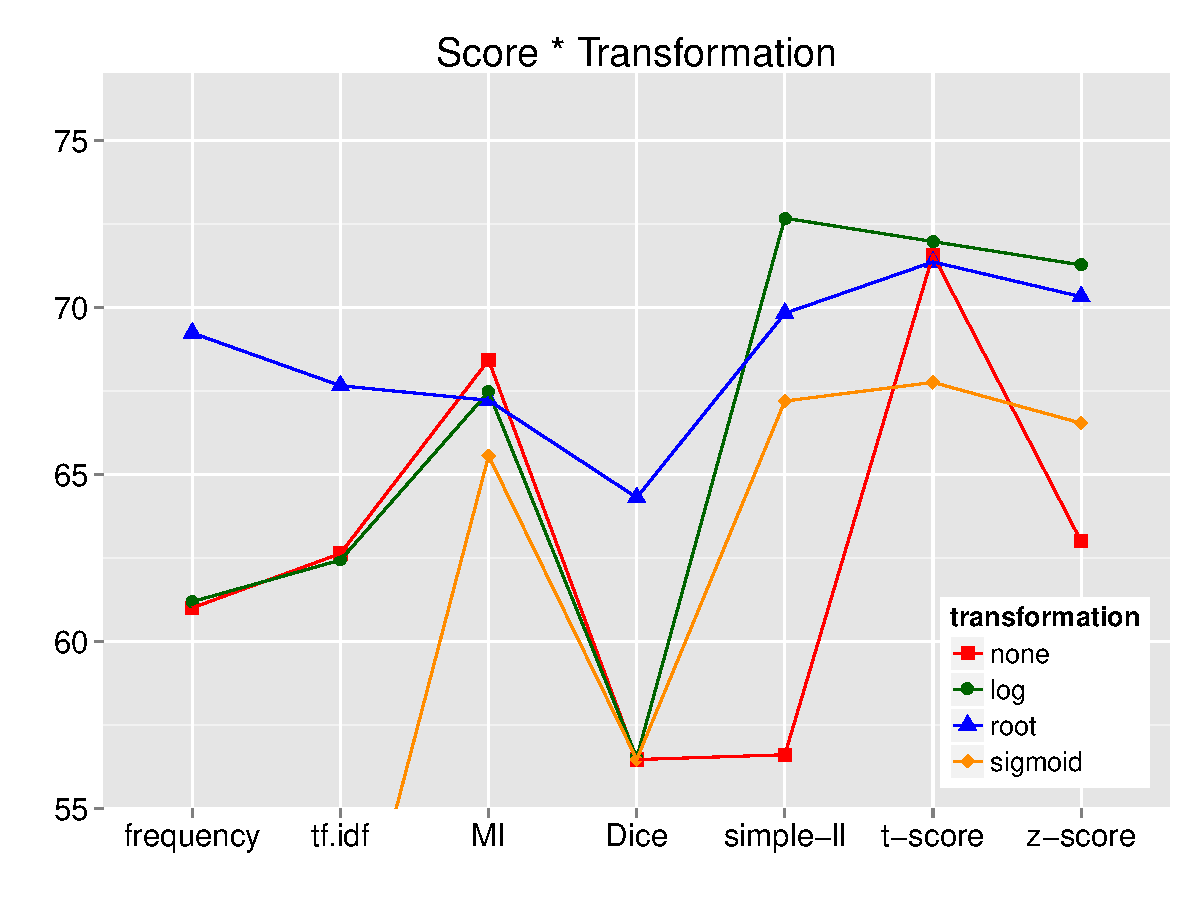
\includegraphics[scale=0.48]{img/lapesa_toefl_main_score_transformation}}%
  \only<beamer:2| handout:0>{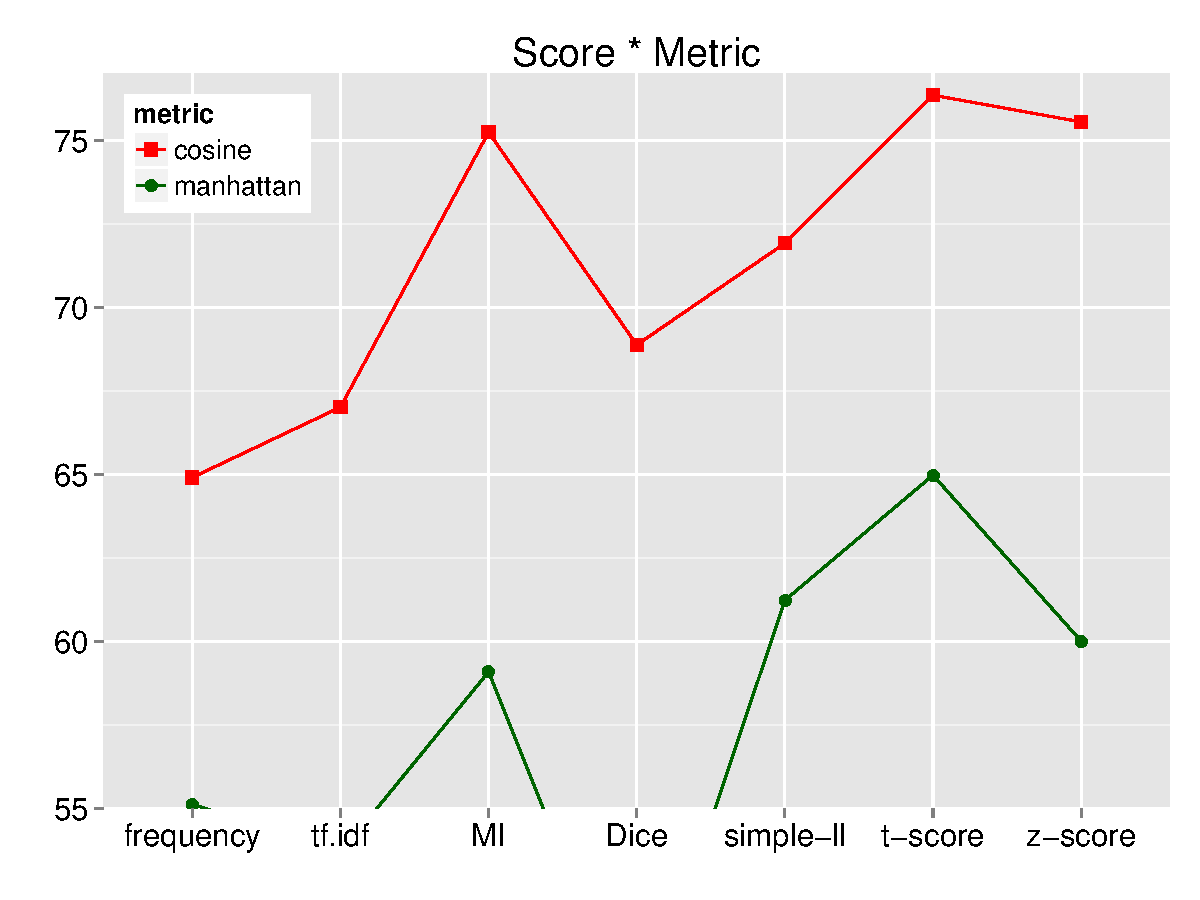
\includegraphics[scale=0.48]{img/lapesa_toefl_main_score_metric}}%
  \only<beamer:0| handout:1>{
    \gap[1]\hspace*{-1cm}%
    \begin{tabular}{c@{}c}
      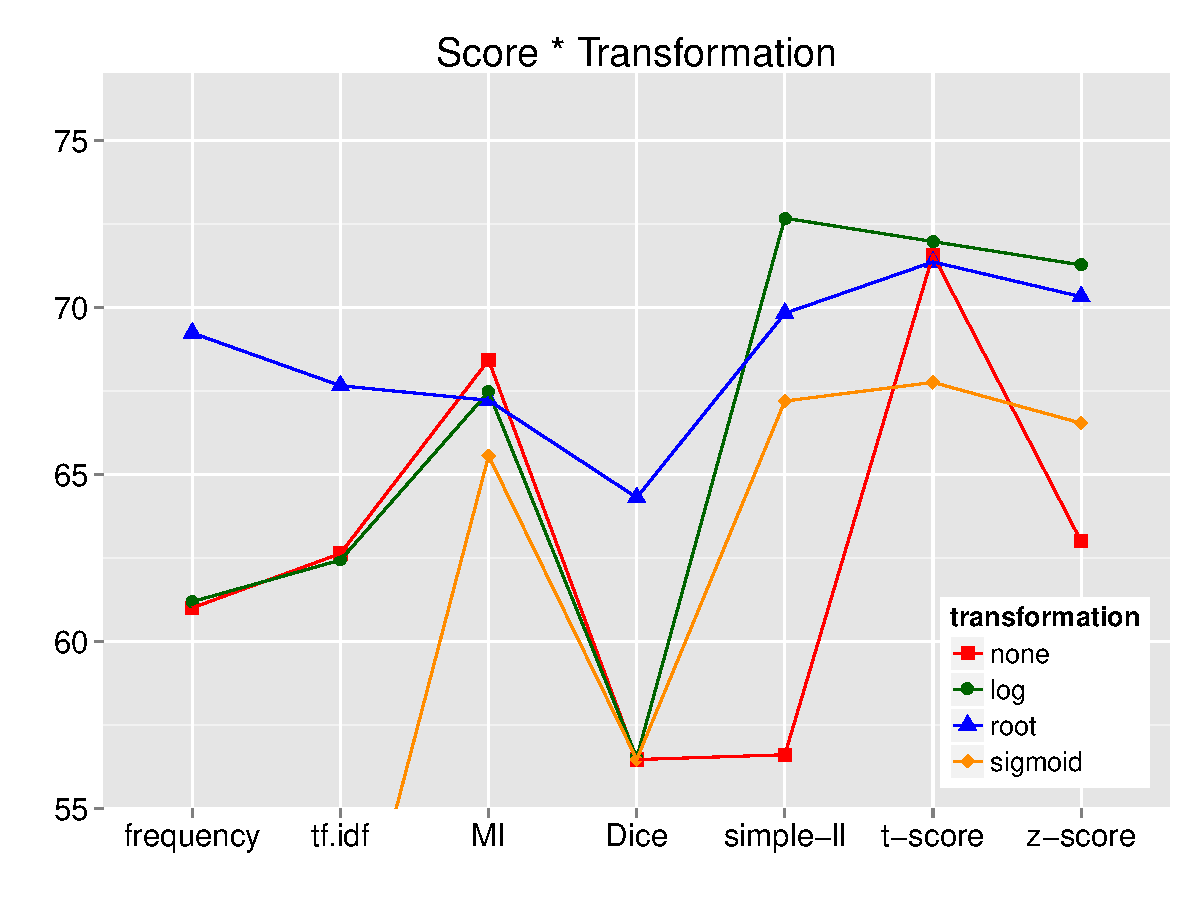
\includegraphics[scale=0.30]{img/lapesa_toefl_main_score_transformation} &
      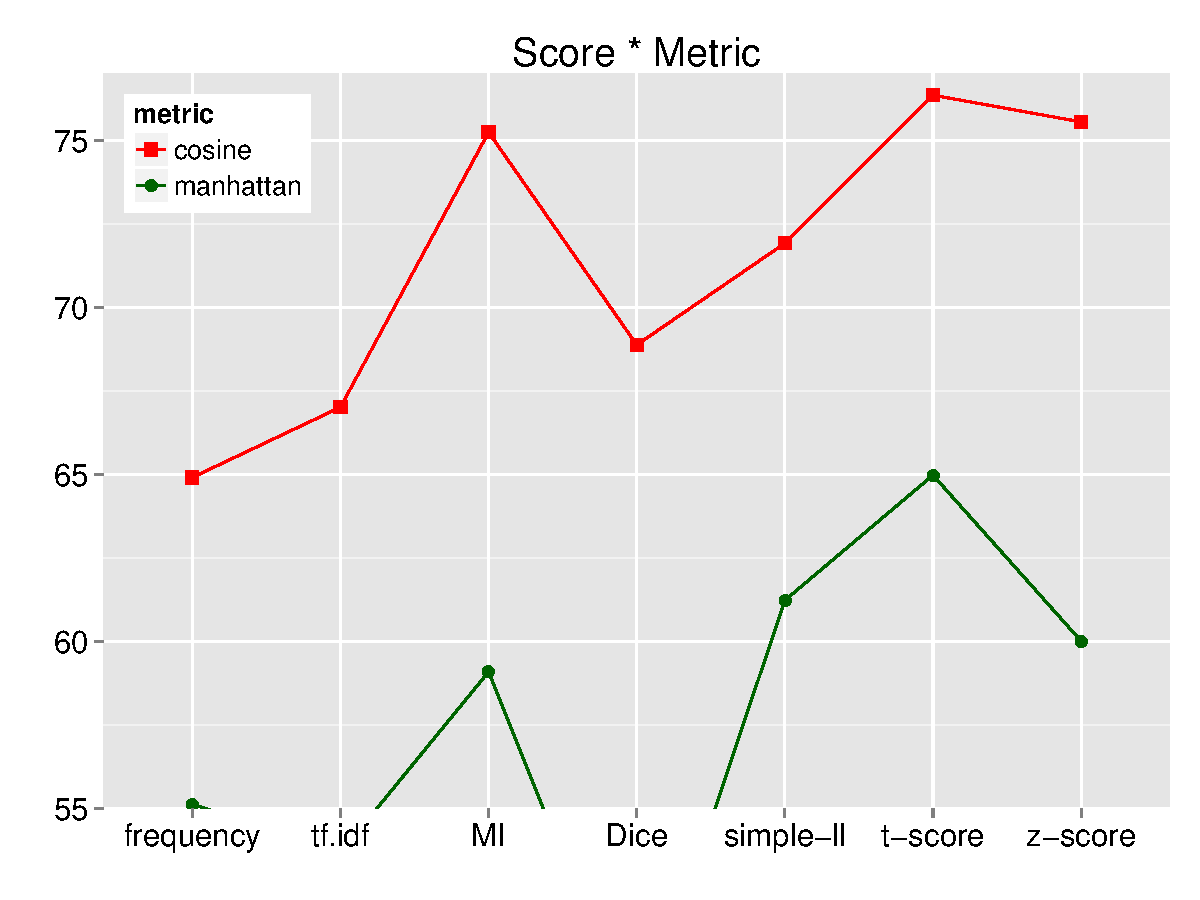
\includegraphics[scale=0.30]{img/lapesa_toefl_main_score_metric}
    \end{tabular}
  }
\end{frame}

\begin{frame}
  \frametitle{TOEFL task: Dimensionality Reduction}
  \framesubtitle{Partial effect displays \citep{Fox:03}} 

  \centering
  \only<beamer:1-2| handout:0>{\ungap[1]}%
  \only<beamer:1| handout:0>{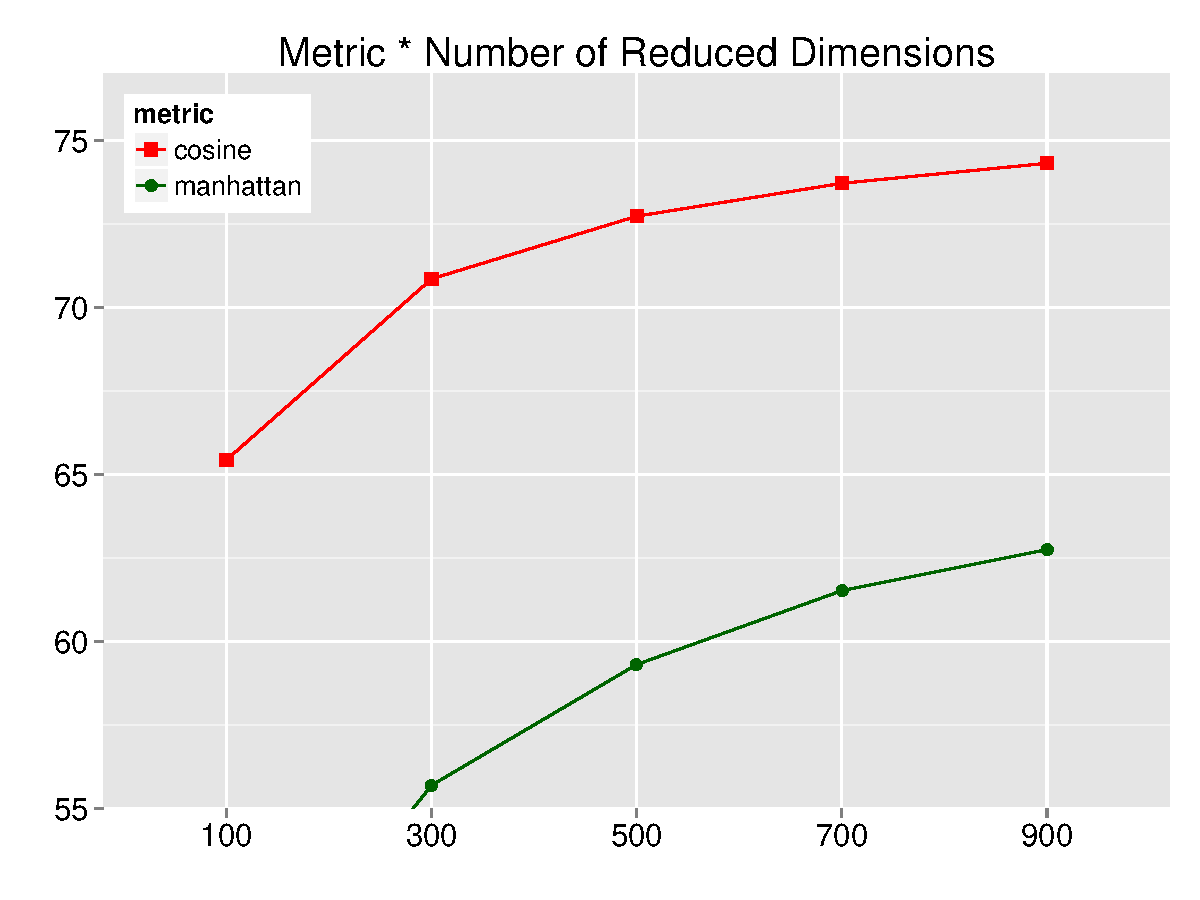
\includegraphics[scale=0.48]{img/lapesa_toefl_main_metric_n-dim}}%
  \only<beamer:2| handout:0>{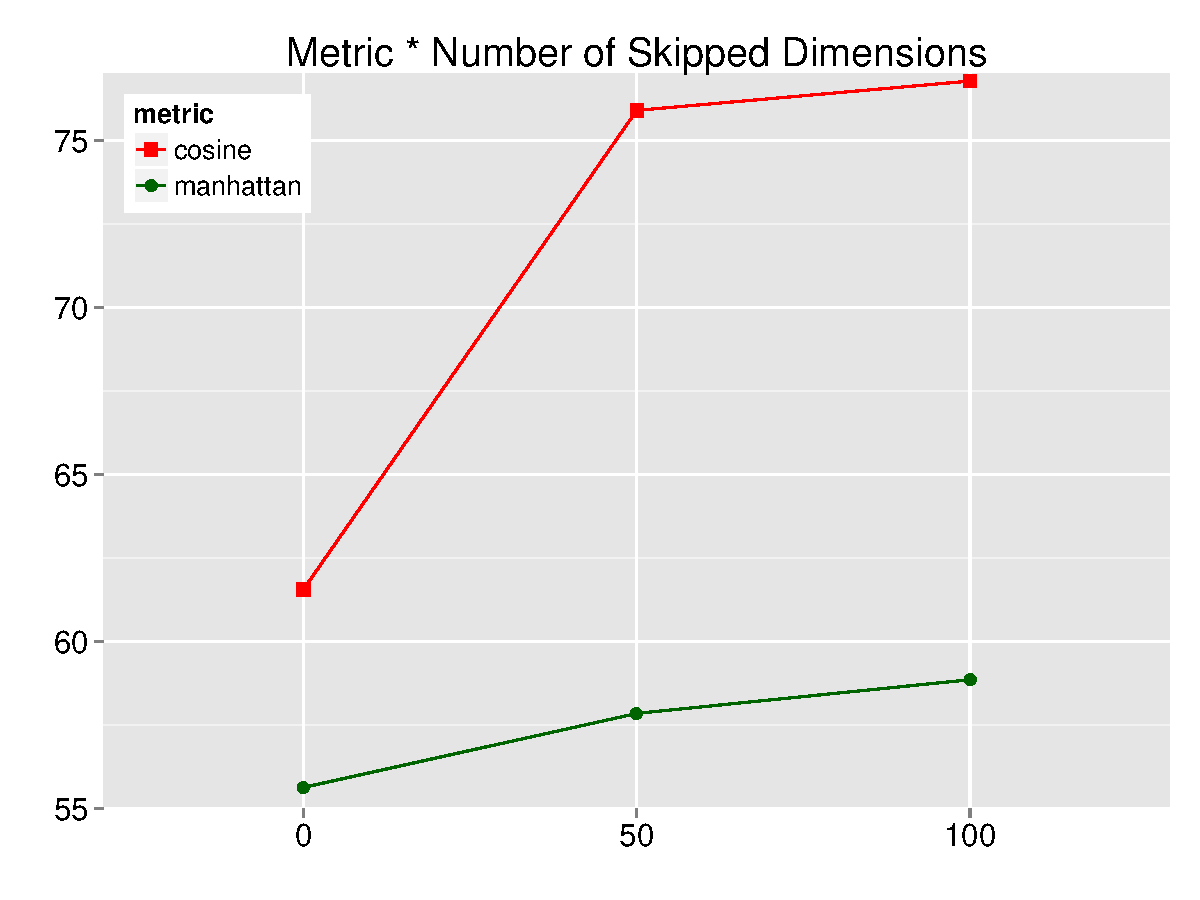
\includegraphics[scale=0.48]{img/lapesa_toefl_main_metric_dim-skip}}%
  \only<beamer:0| handout:1>{
    \gap[1]\hspace*{-1cm}%
    \begin{tabular}{c@{}c}
      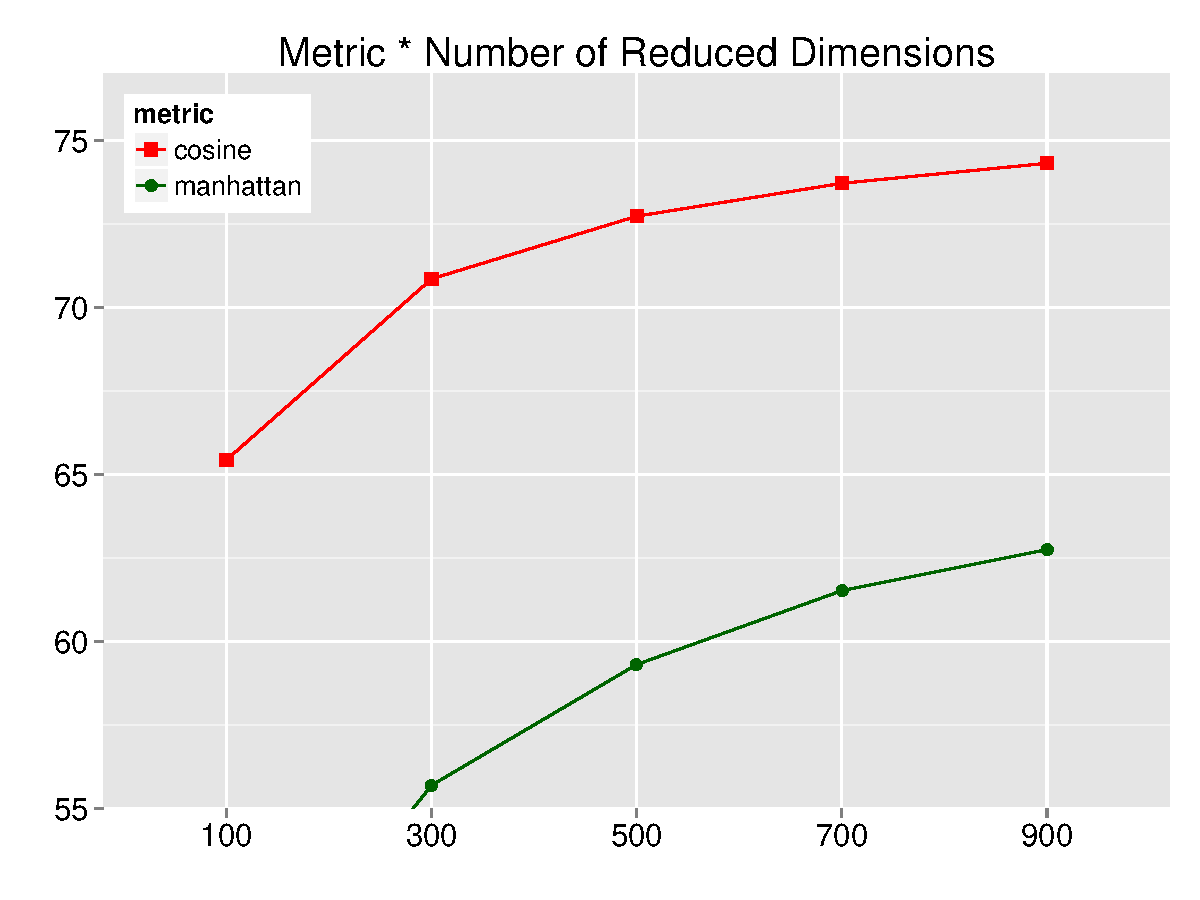
\includegraphics[scale=0.30]{img/lapesa_toefl_main_metric_n-dim} &
      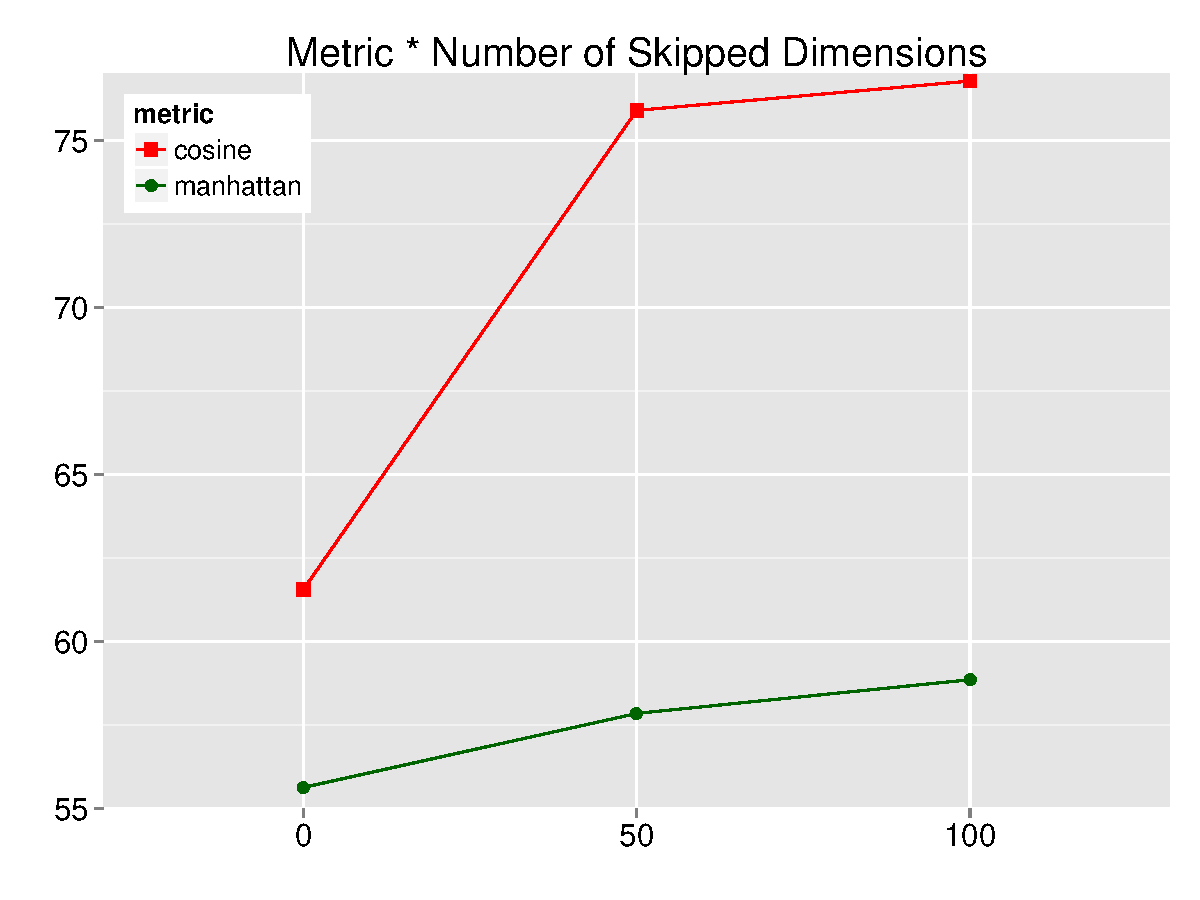
\includegraphics[scale=0.30]{img/lapesa_toefl_main_metric_dim-skip}
    \end{tabular}
  }
\end{frame}

\begin{frame}
  \frametitle{TOEFL task: Corpus and Number of Feature Dimensions}
  \framesubtitle{Partial effect displays \citep{Fox:03}} 

  \centering
  \only<beamer:1-2| handout:0>{\ungap[1]}%
  \only<beamer:1| handout:0>{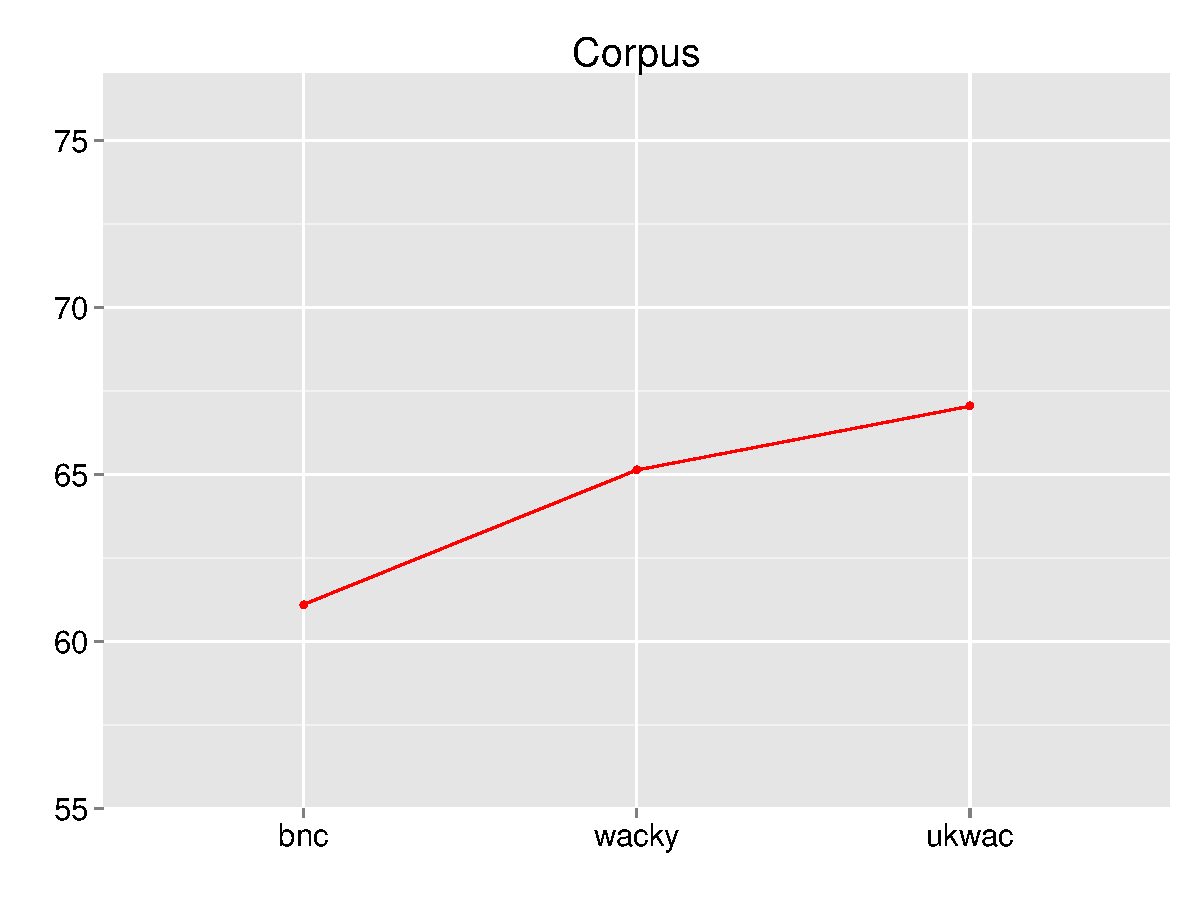
\includegraphics[scale=0.48]{img/lapesa_toefl_main_corpus}}%
  \only<beamer:2| handout:0>{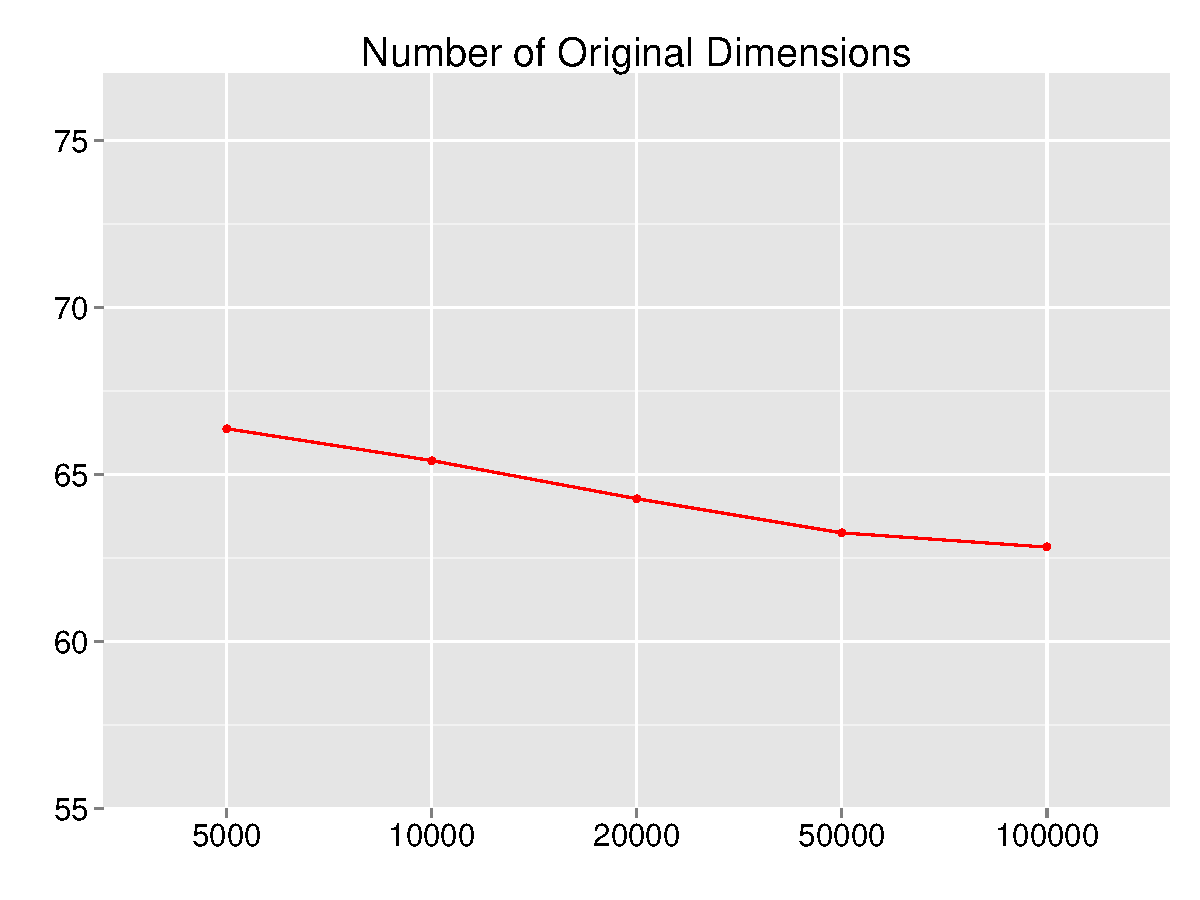
\includegraphics[scale=0.48]{img/lapesa_toefl_main_origdim}}%
  \only<beamer:0| handout:1>{
    \gap[1]\hspace*{-1cm}%
    \begin{tabular}{c@{}c}
      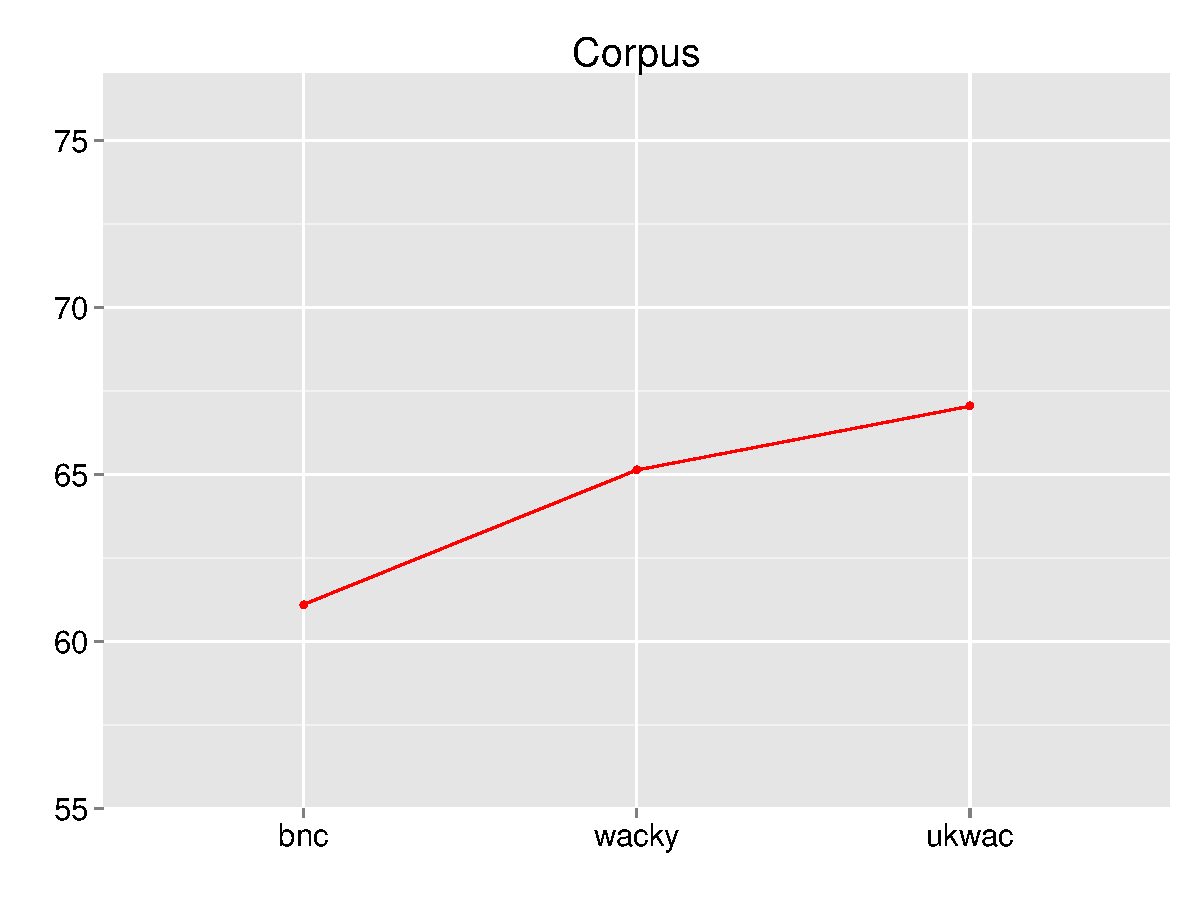
\includegraphics[scale=0.30]{img/lapesa_toefl_main_corpus} &
      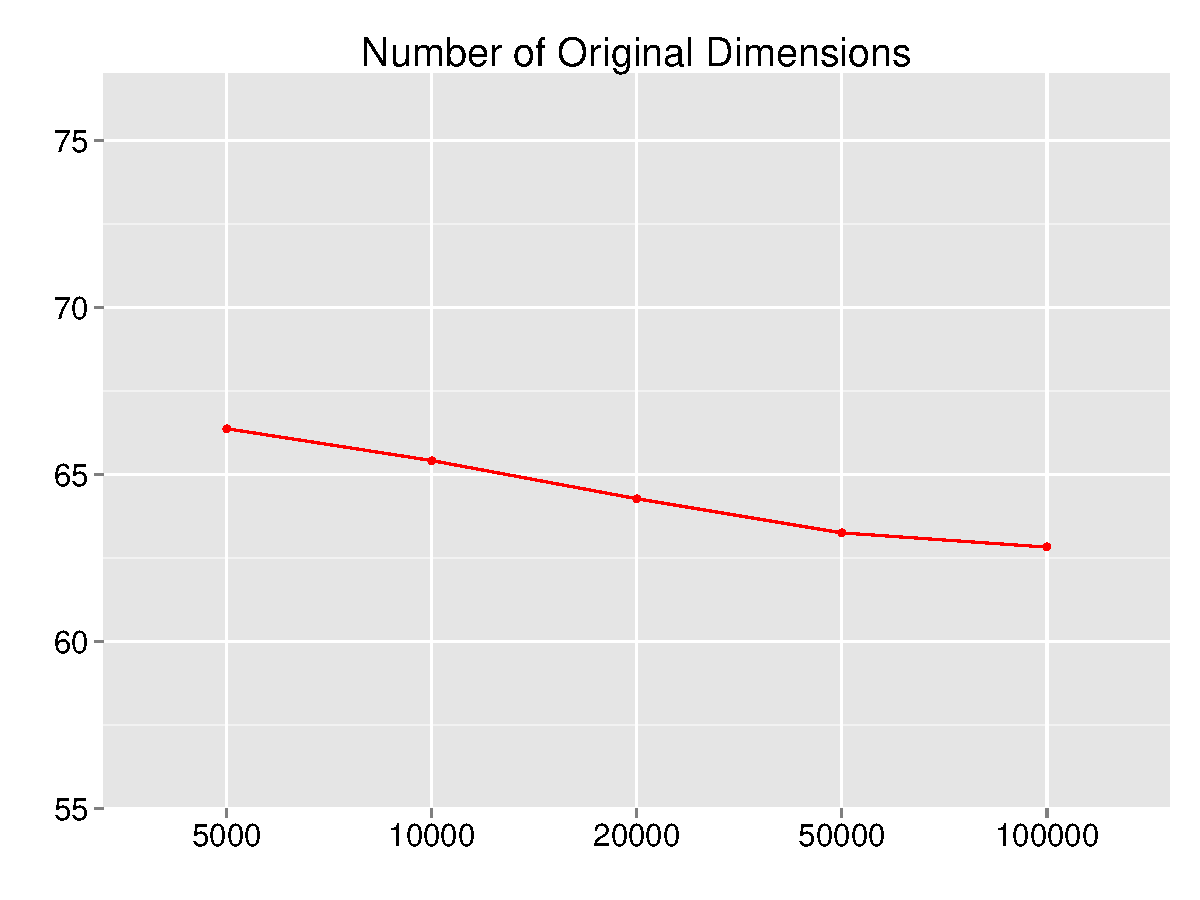
\includegraphics[scale=0.30]{img/lapesa_toefl_main_origdim}
    \end{tabular}
  }
\end{frame}

\begin{frame}
  \frametitle{TOEFL task: Window and Relatedness Index}
  \framesubtitle{Partial effect displays \citep{Fox:03}} 

  \centering
  \only<beamer:1-2| handout:0>{\ungap[1]}%
  \only<beamer:1| handout:0>{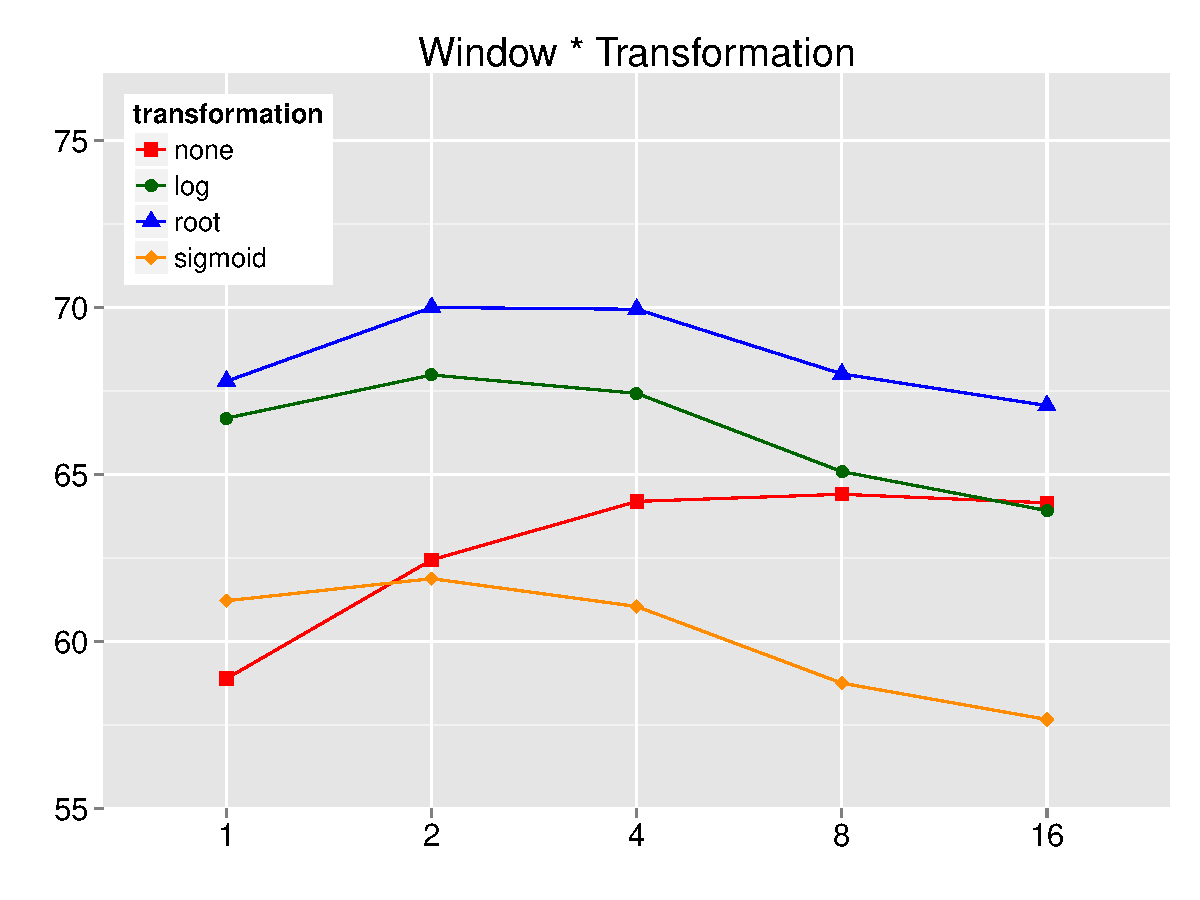
\includegraphics[scale=0.48]{img/lapesa_toefl_main_window_transformation}}%
  \only<beamer:2| handout:0>{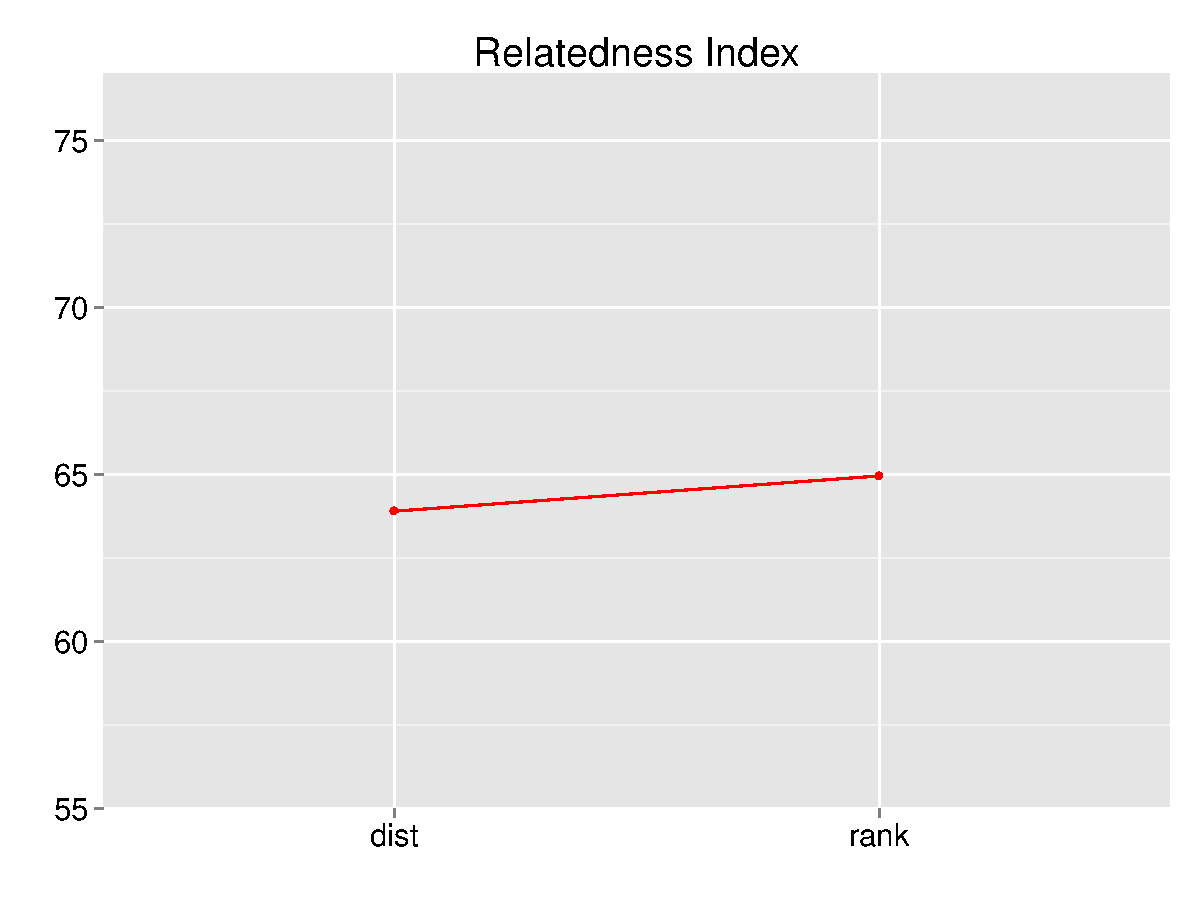
\includegraphics[scale=0.48]{img/lapesa_toefl_main_relindex}}%
  \only<beamer:0| handout:1>{
    \gap[1]\hspace*{-1cm}%
    \begin{tabular}{c@{}c}
      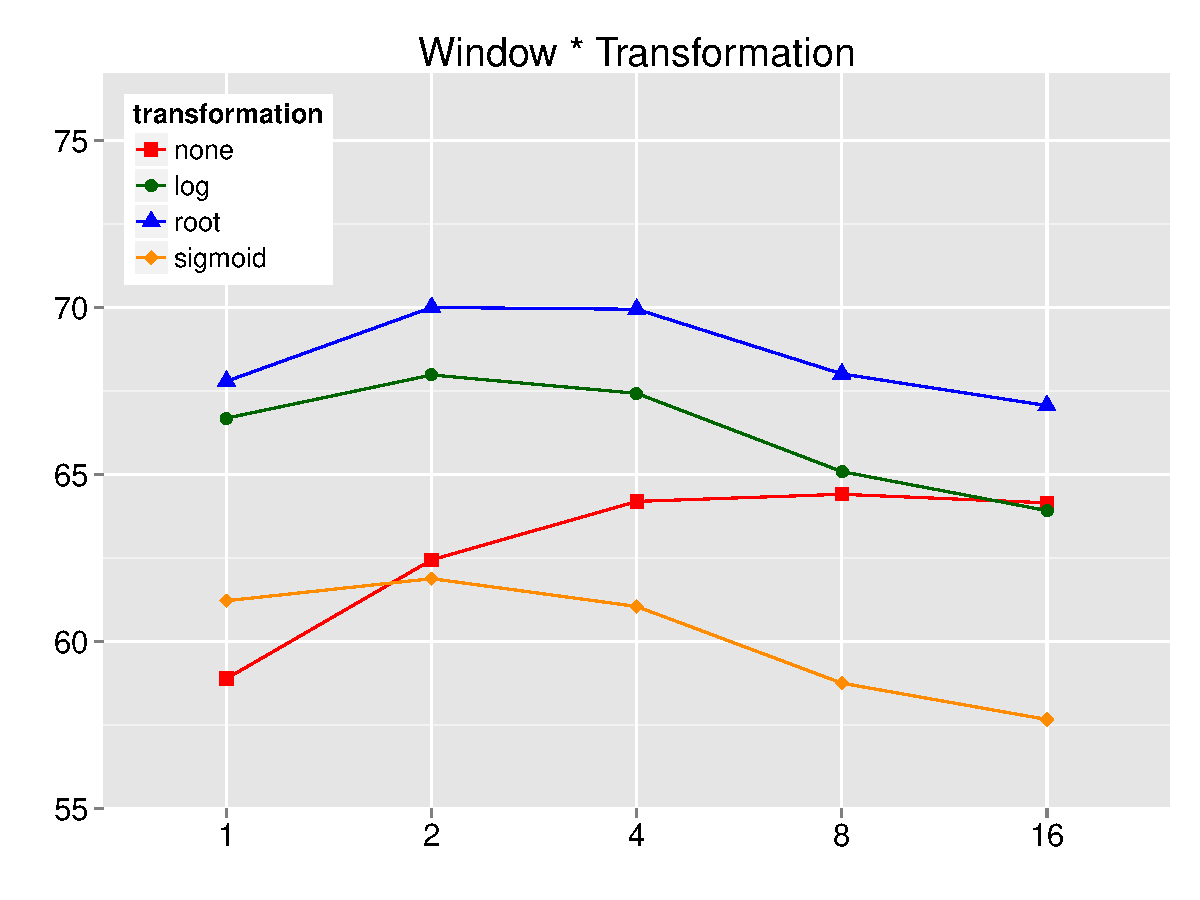
\includegraphics[scale=0.30]{img/lapesa_toefl_main_window_transformation} &
      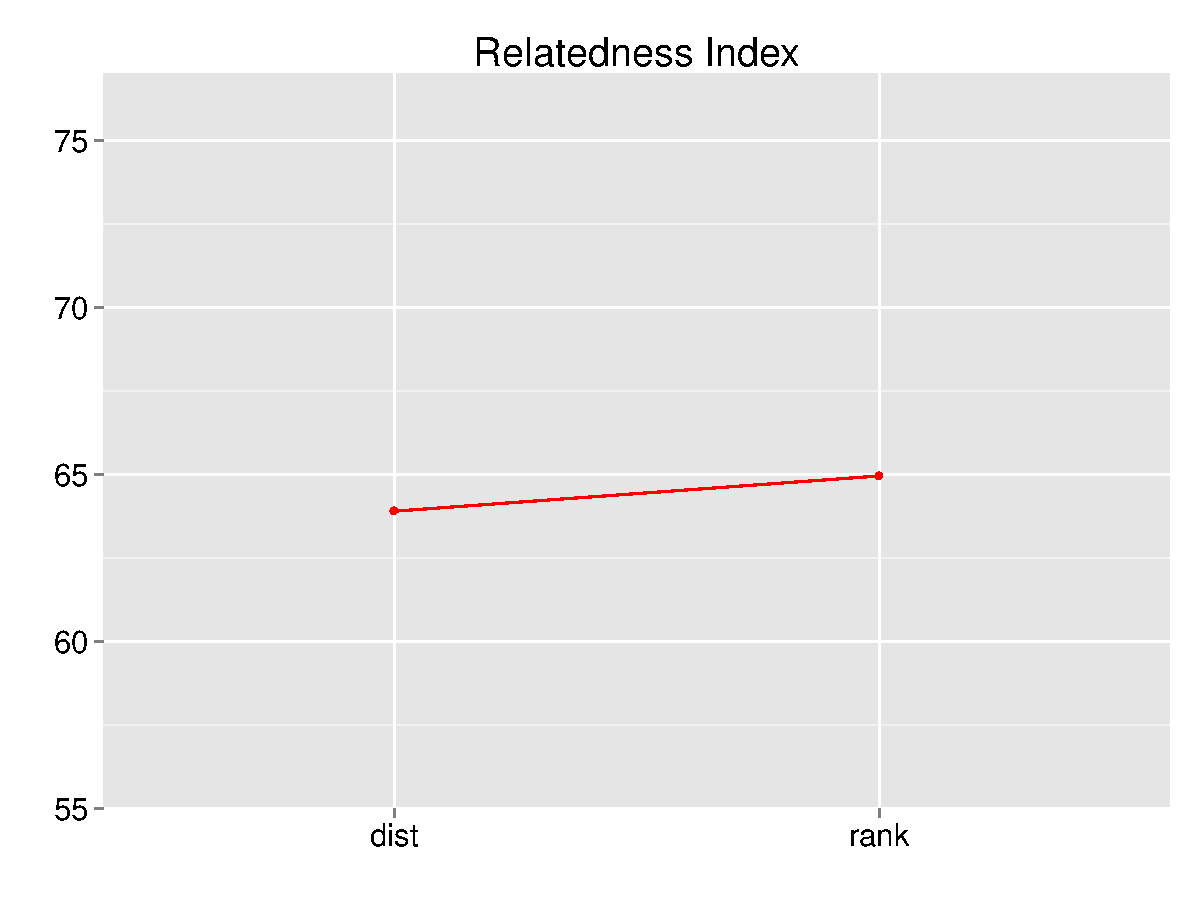
\includegraphics[scale=0.30]{img/lapesa_toefl_main_relindex}
    \end{tabular}
  }
\end{frame}

\begin{frame}
  \frametitle{TOEFL task: summary}
  \begin{exampleblock}{TOEFL: best setting}
    \begin{itemize}\footnotesize
    \item Corpus: ukWac
    \item Window: undirected, 2 words 
    \item Feature selection: top 5000/10000 dimensions, based on frequency
    \item Score * Transformation: simple-ll * log
    \item Dimensionality Reduction: 900 latent dimensions, skipping the first 100
    \item Distance Metric: cosine
    \item Index of Distributional Relatedness: neighbor rank
    \end{itemize}
  \end{exampleblock}   
  
\end{frame}


\begin{frame}
  \frametitle{DSMs and similarity ratings}
  \framesubtitle{Introducing the task}

  \ungap[1]
  \begin{columns}
    \begin{column}{0.5\textwidth}
      \begin{exampleblock}{RG65}
        \textbf{65 pairs, rated from 0 to 4}
        \textit{gem -- jewel}: 3.94 \\
        \textit{grin -- smile}:  3.46 \\
        \textit{fruit -- furnace}: 0.05 \\
      \end{exampleblock}
    \end{column}
    % 
    \begin{column}{0.5\textwidth}
      
      
      \begin{exampleblock}  {WordSim353}
        \textbf{353 pairs, rated from 1 to 10}
        \textit{announcement -- news}: 7.56 \\
        \textit{weapon -- secret}:  6.06 \\
        \textit{travel -- activity}: 5.00 \\
      \end{exampleblock}
    \end{column}
    % 
  \end{columns}
  % 
  % 
  \begin{itemize}
  \item A \textbf{prediction} task
  \item If distributional representation are close to  speakers' conceptual representations, we expect to find some \textbf{correlation} between distance in the semantic space and speaker's judgments concerning semantic similarity
  \item Performance: \textbf{Pearson correlation $r$}
  \end{itemize}

\end{frame}

\begin{frame}
  \frametitle{Similarity ratings: performance on RG65}
  \centering
  
  \begin{columns}
    \begin{column}{0.5\textwidth}
      \centering
      \hspace*{-18pt}   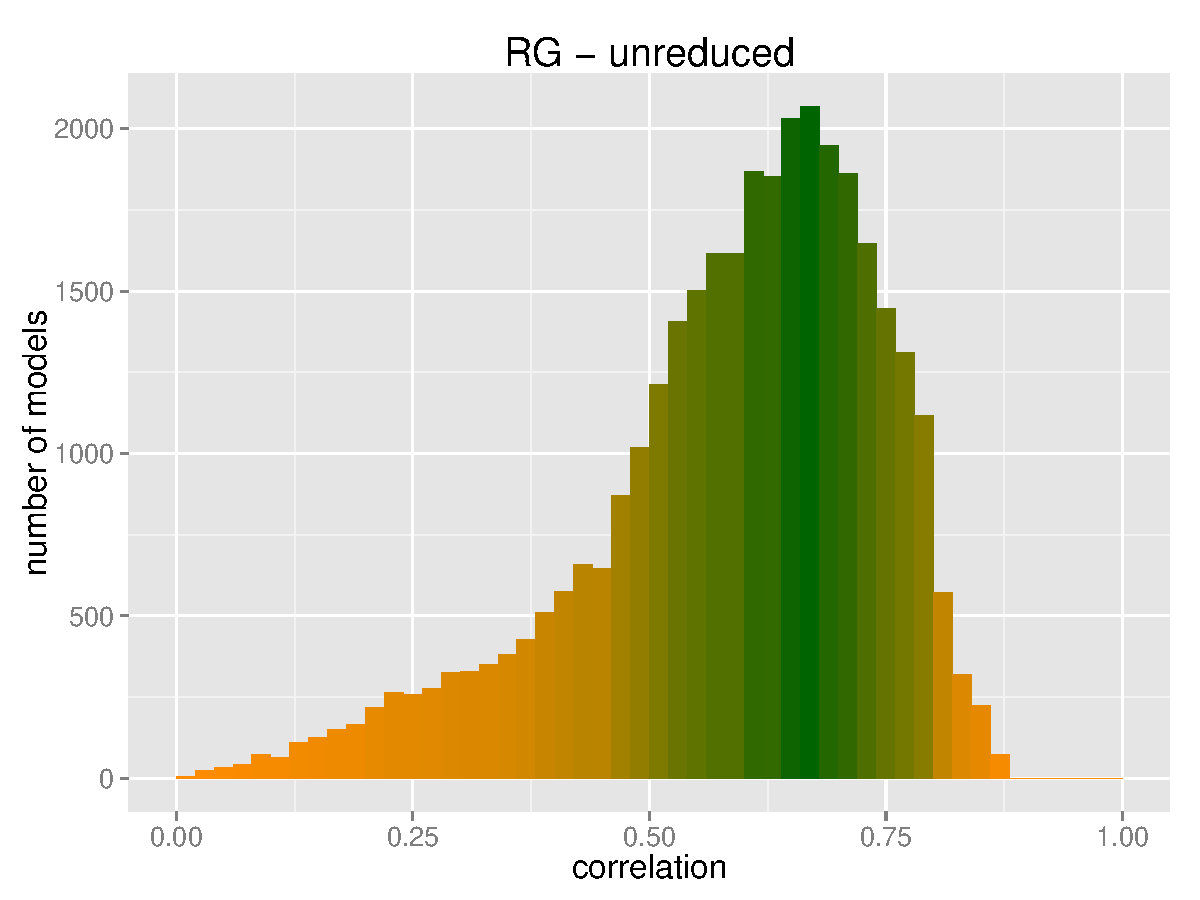
\includegraphics[scale=0.30]{img/lapesa_hist_rg_unreduced}
      \begin{block}{}\footnotesize \centering
        Min:  0.01; Max:  0.88;  Mean 0.59 \\
        \secondary{unreduced}
      \end{block}
    \end{column}
    \begin{column}{0.5\textwidth}
      \hspace*{-18pt} 
      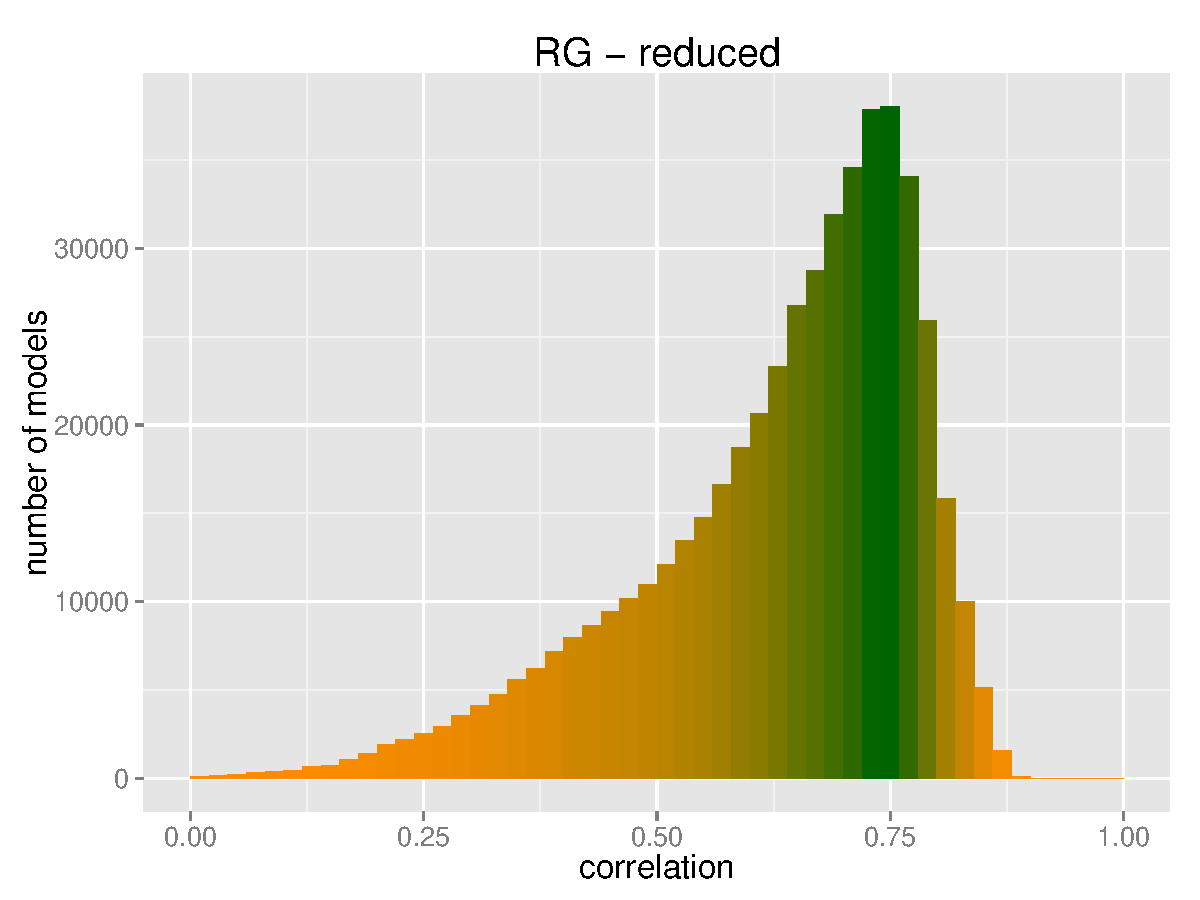
\includegraphics[scale=0.30]{img/lapesa_hist_rg_reduced}
      \begin{block}{}\footnotesize \centering
        Min:  0.00; Max: \primary{0.89};  Mean: 0.63\\
        \secondary{reduced}
      \end{block}
    \end{column}
  \end{columns}
 
\end{frame}

\begin{frame}
  \frametitle{Similarity ratings: performance on WordSim353}
  \centering
  
  \begin{columns}

    \begin{column}{0.5\textwidth}
      \centering
      \hspace*{-18pt} 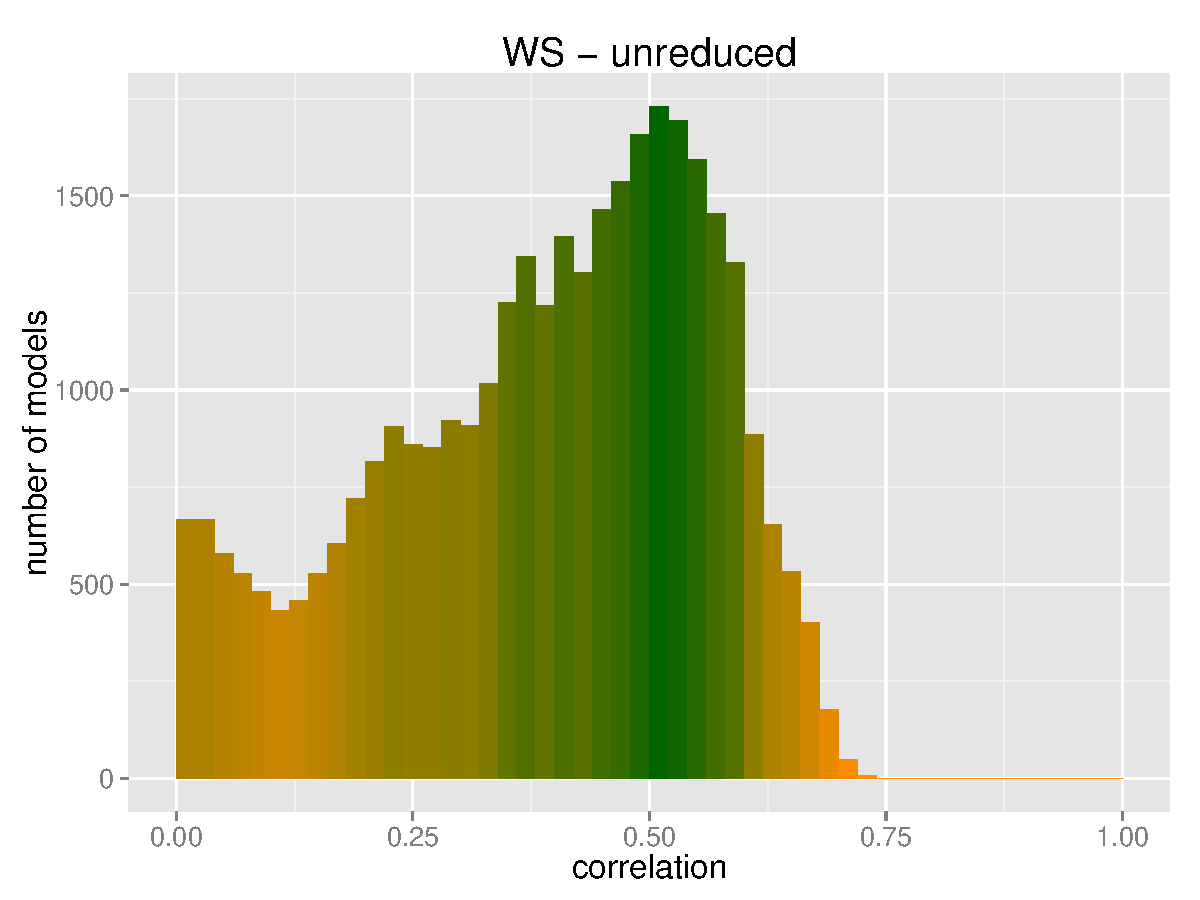
\includegraphics[scale=0.30]{img/lapesa_hist_ws_unreduced}
      \begin{block}{}\footnotesize \centering
        Min:  0.00; Max: \primary{0.73};  Mean: 0.39\\
        \secondary{unreduced}
      \end{block}
    \end{column}
    \begin{column}{0.5\textwidth}
      \hspace*{-18pt} 
      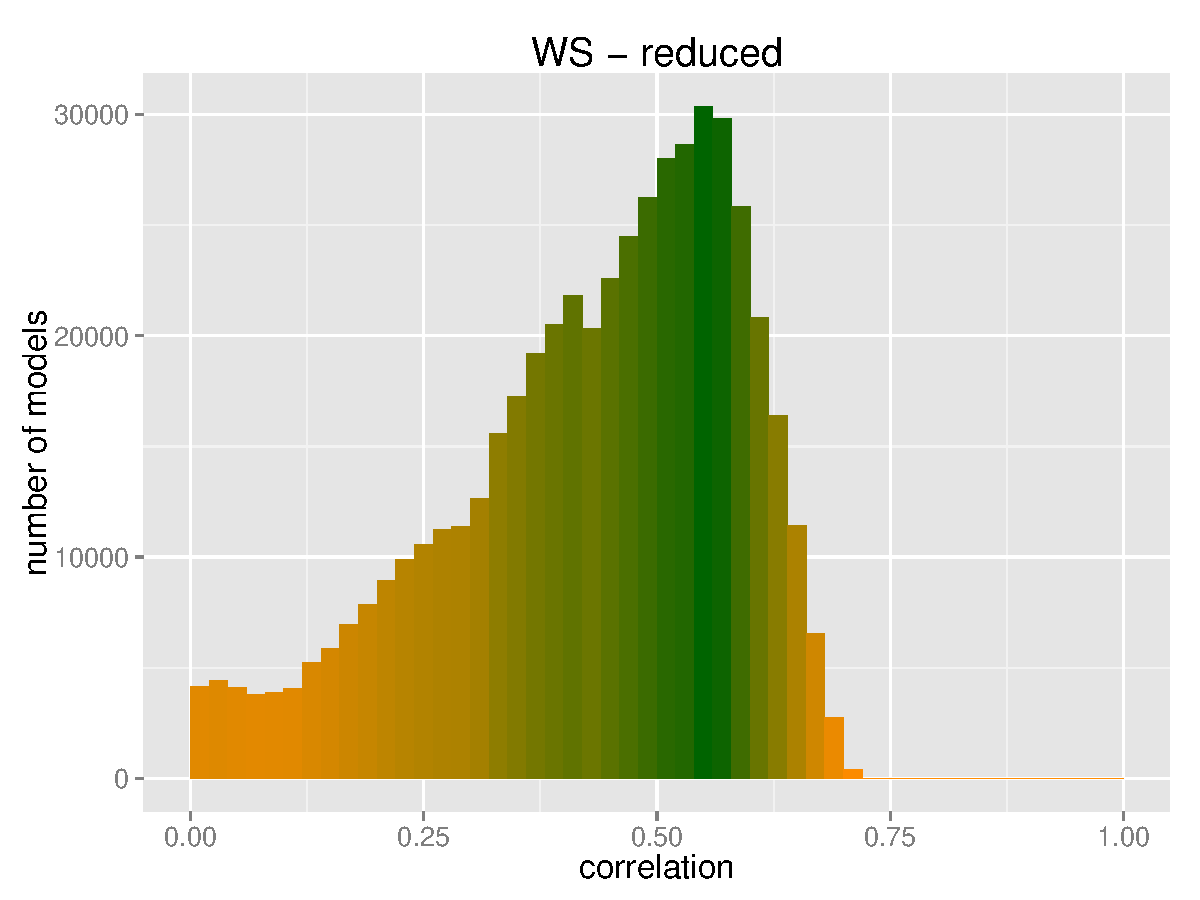
\includegraphics[scale=0.30]{img/lapesa_hist_ws_reduced}
      \begin{block}{}\footnotesize \centering
        Min:  0.00; Max: \primary{0.73};  Mean: 0.43\\
        \secondary{reduced}
      \end{block}
    \end{column}
  \end{columns}  
\end{frame}


\begin{frame}
  \frametitle{Similarity ratings: parameters and explained variance}
  \framesubtitle{Reduced setting: feature ablation  (full model $R^{2}$: RG65 86\%; WS353 90\%)}
  \centering
  \hspace*{-10pt}
  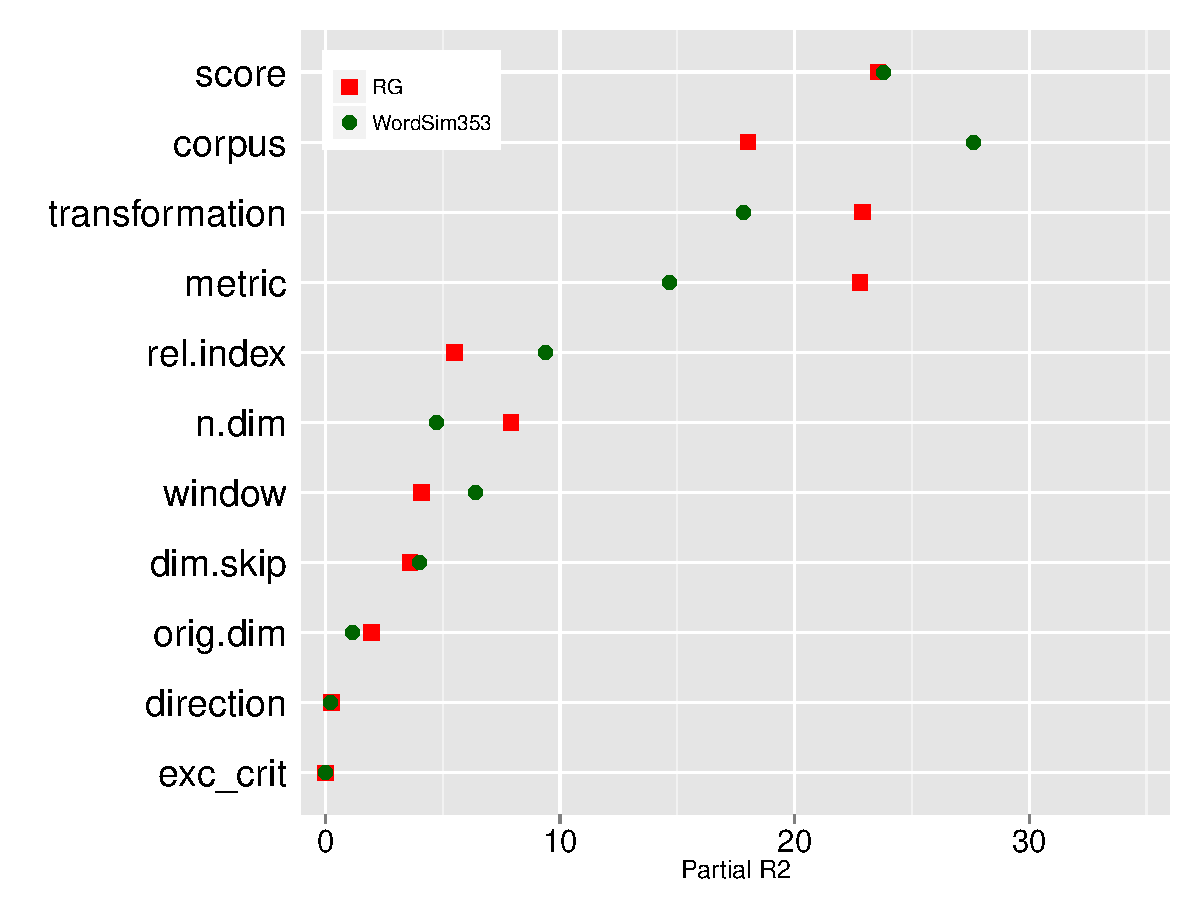
\includegraphics[scale=0.45]{img/lapesa_ratings_main_r2_reduced}
\end{frame}

\begin{frame}
  \frametitle{Similarity ratings: interactions}
  \framesubtitle{Reduced setting ($R^2 > 0.5$)}

  \begin{center}
    \begin{tabular}{lrrrr}
      Interaction & Df & RG65  & WordSim353 \\ \hline

      \primary{score:transf} & 18  & 10.28 & 8.66  \\ 
      \primary{metric:n.dim} & 4  & 2.18 & 1.42 \\   
      \primary{window:transf} & 12  & 1.43 & 1.01 \\   
      corpus:metric & 2  & 1.83 & 0.51 \\  
      score:metric & 6  & 1.91 & 0.59  \\  
      metric:orig.dim & 4  & 1.08 & 0.62 \\ 
      corpus:score & 12 & 0.77 &  0.82 \\ 
      window:score & 24  & 0.77 & 0.69  \\
      score:dim.skip & 12  & 0.58 & 0.85 \\ 
    \end{tabular}

    \gap[1]
    \secondary{Similarity ratings: interactions, $R^2$} 
  \end{center}

\end{frame}


\begin{frame}
  \frametitle{Similarity ratings: Score, Transformation}
  \framesubtitle{Partial effect displays \citep{Fox:03}} 

  \centering
  \gap[1]\hspace*{-1cm}%
  \begin{tabular}{c@{}c}
    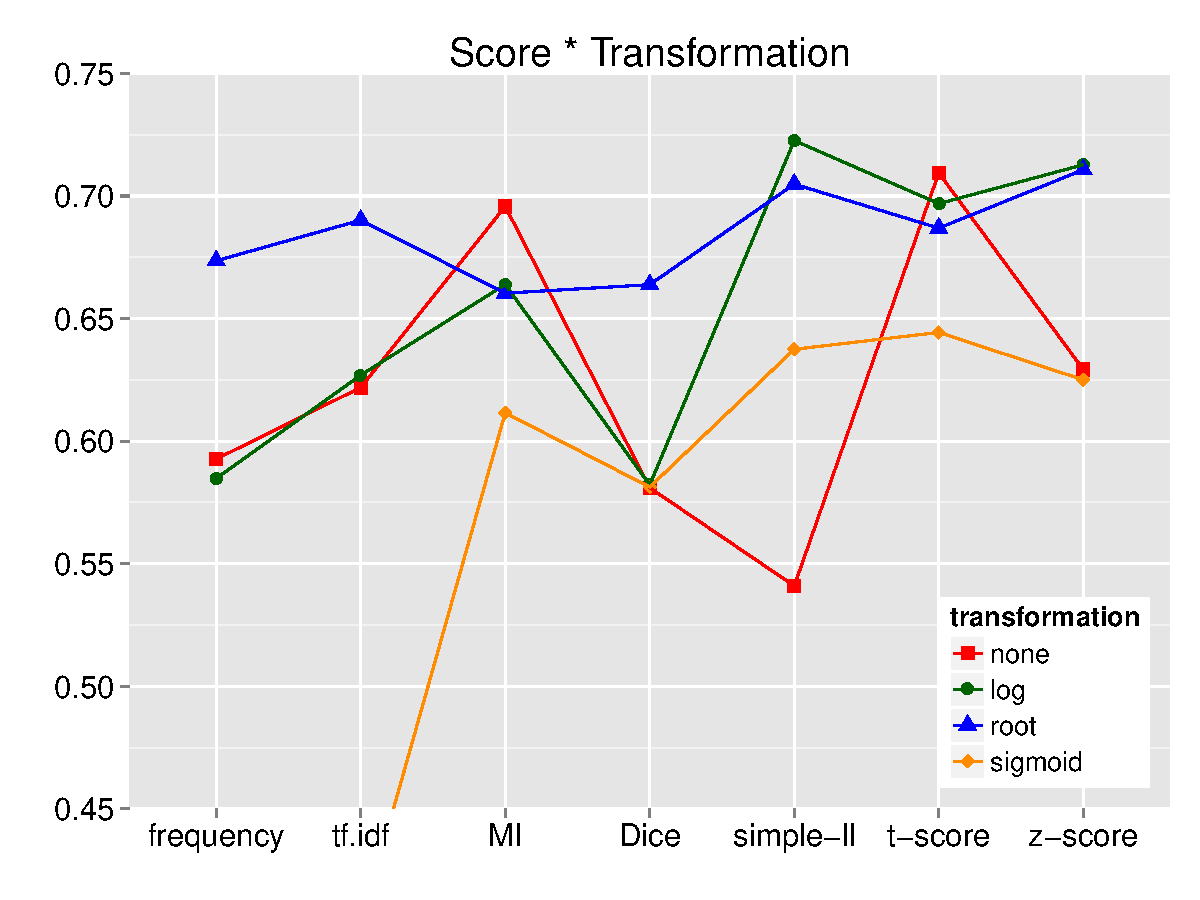
\includegraphics[scale=0.30]{img/lapesa_rg_main_score_transformation} &
    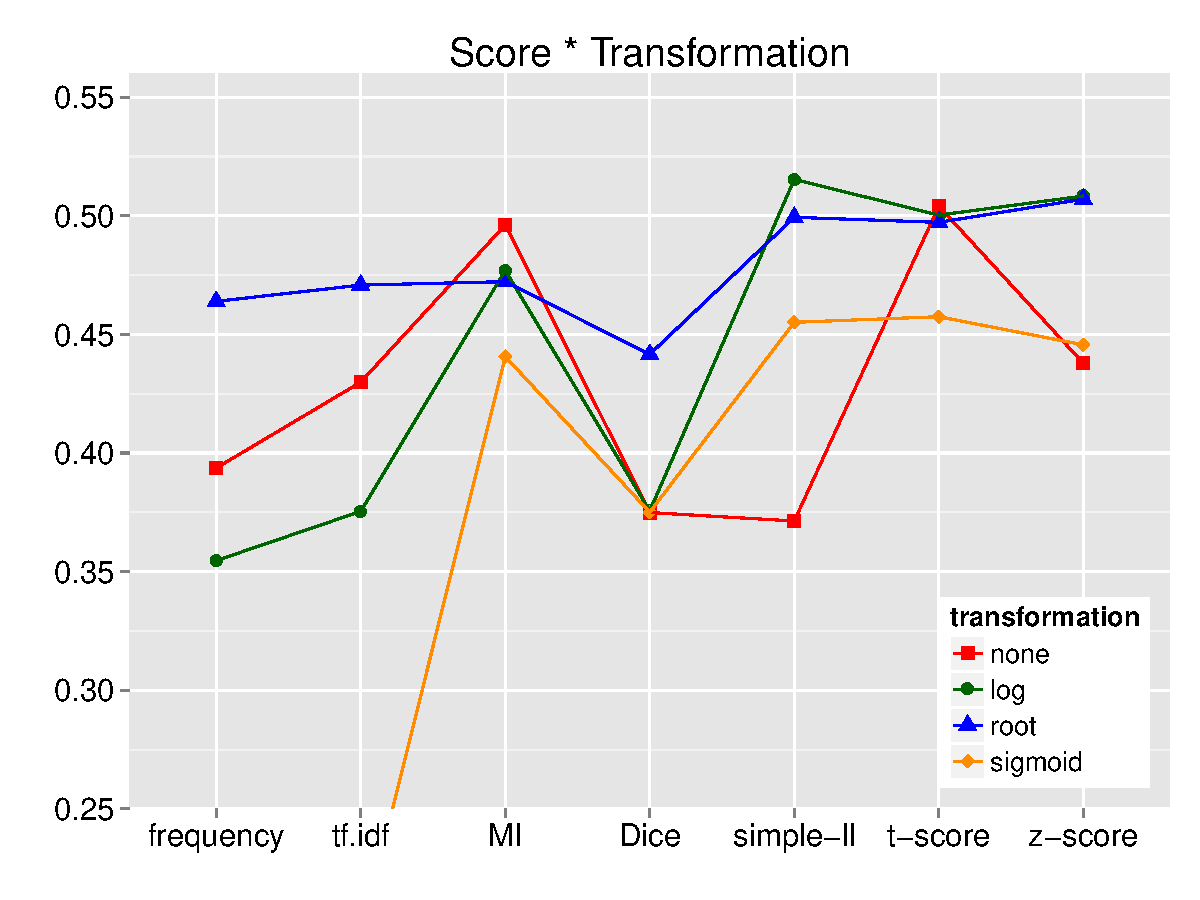
\includegraphics[scale=0.30]{img/lapesa_ws_main_score_transformation} \\
    \secondary{Rubenstein \& Goodenough} &
    \secondary{WordSim-353}
  \end{tabular}
\end{frame}


\begin{frame}
  \frametitle{Similarity ratings: Relatedness Index}
  \framesubtitle{Partial effect displays \citep{Fox:03}} 

  \centering
  \gap[1]\hspace*{-1cm}%
  \begin{tabular}{c@{}c}
    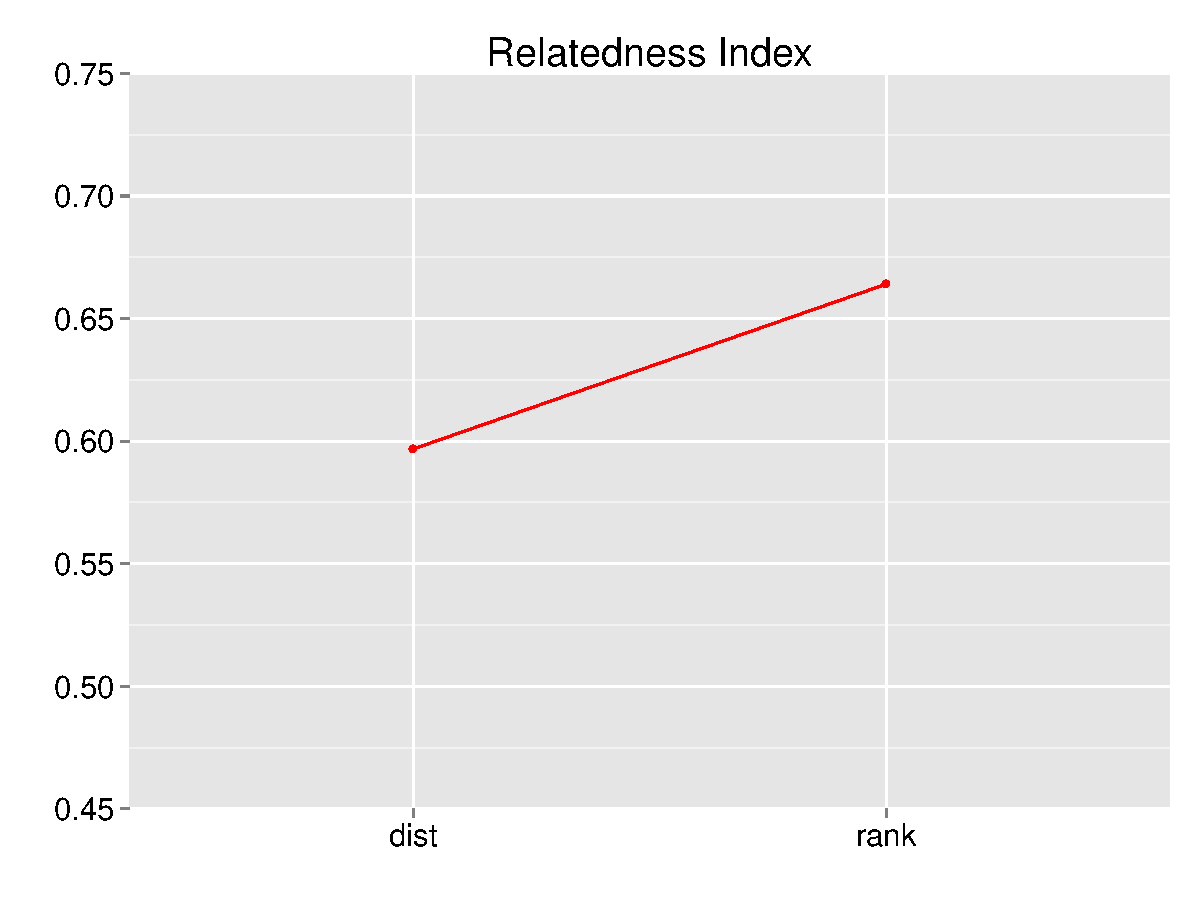
\includegraphics[scale=0.30]{img/lapesa_rg_main_relindex} &
    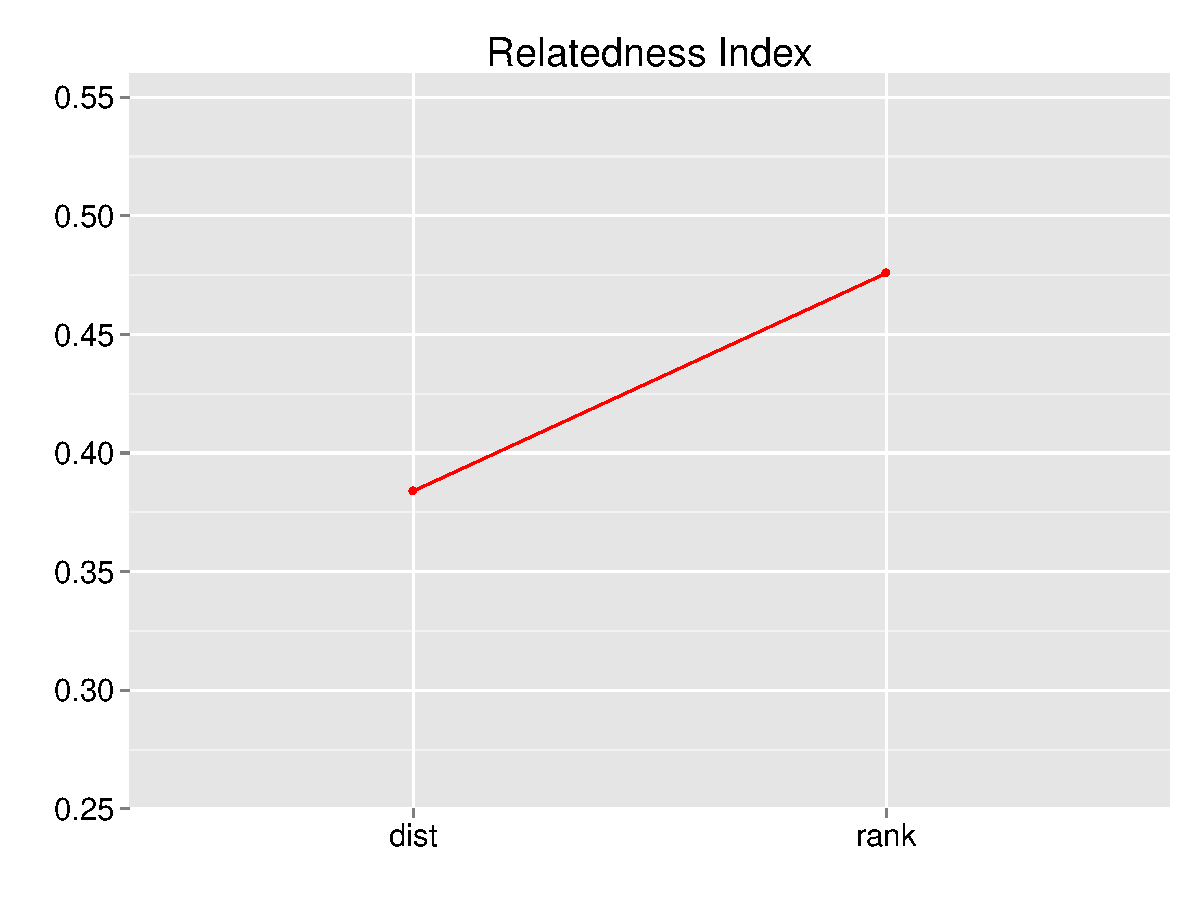
\includegraphics[scale=0.30]{img/lapesa_ws_main_relindex} \\
    \secondary{Rubenstein \& Goodenough} &
    \secondary{WordSim-353}
  \end{tabular}
\end{frame}

\begin{frame}
  \frametitle{Similarity ratings: Metric, Number of Feature Dimensions}
  \framesubtitle{Partial effect displays \citep{Fox:03}} 

  \centering
  \gap[1]\hspace*{-1cm}%
  \begin{tabular}{c@{}c}
    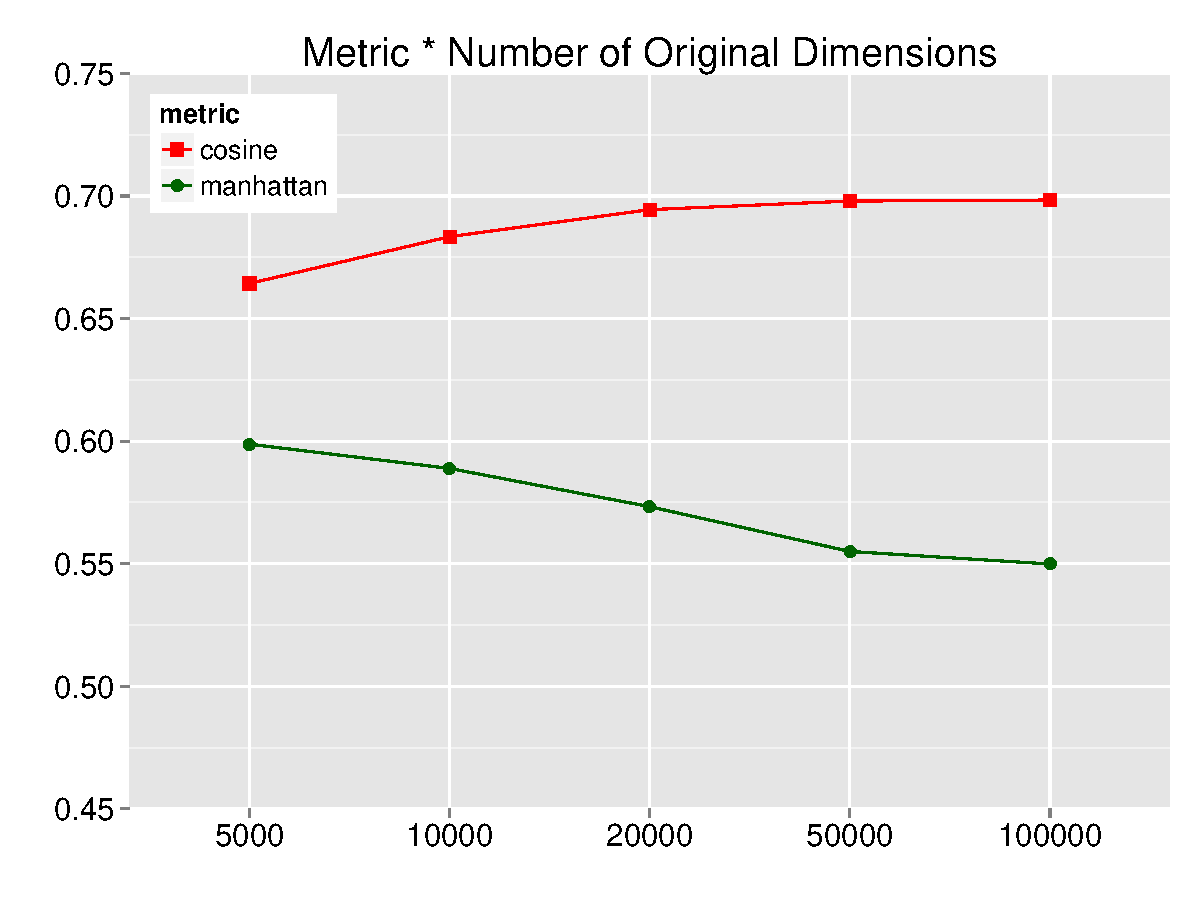
\includegraphics[scale=0.30]{img/lapesa_rg_main_metric_origdim} &
    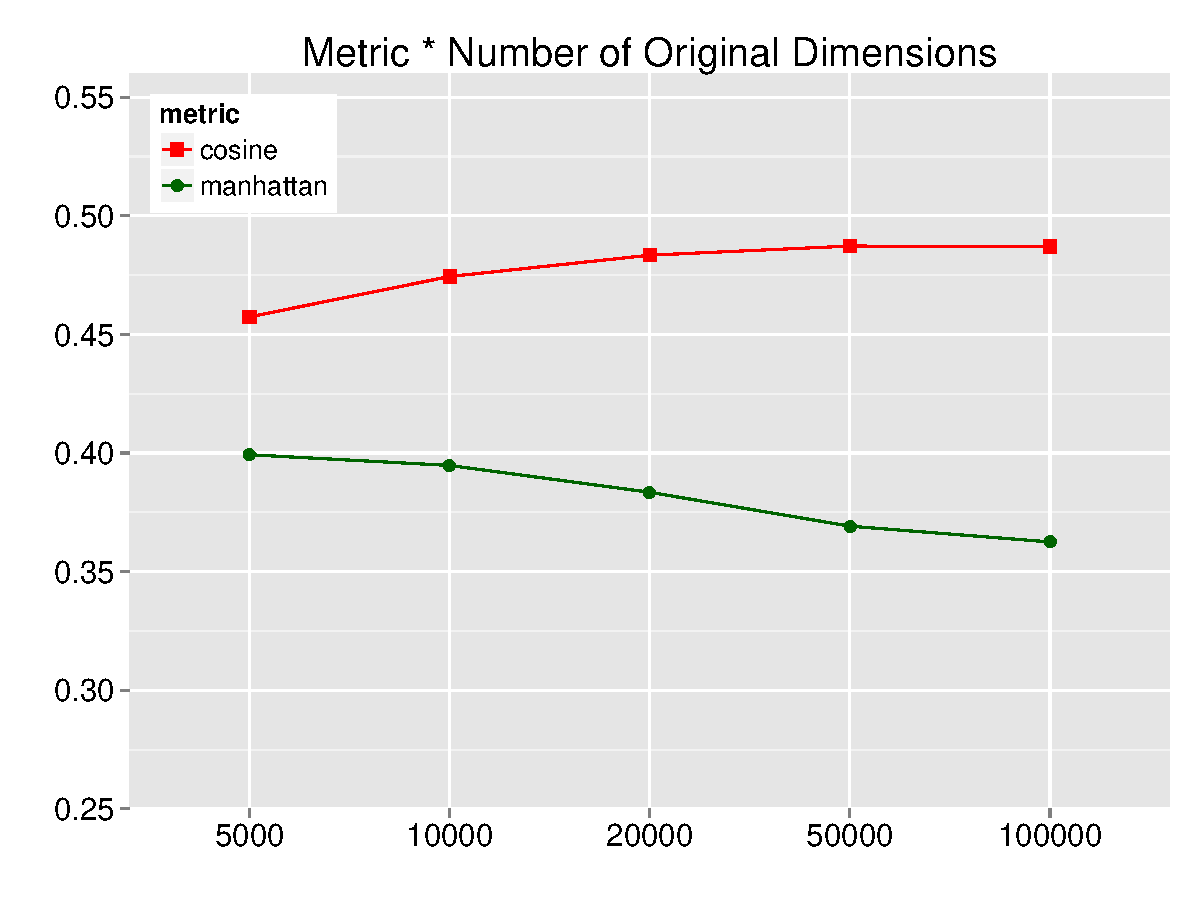
\includegraphics[scale=0.30]{img/lapesa_ws_main_metric_origdim} \\
    \secondary{Rubenstein \& Goodenough} &
    \secondary{WordSim-353}
  \end{tabular}
\end{frame}

\begin{frame}
  \frametitle{Similarity ratings: Number of Latent Dimensions}
  \framesubtitle{Partial effect displays \citep{Fox:03}} 

  \centering
  \gap[1]\hspace*{-1cm}%
  \begin{tabular}{c@{}c}
    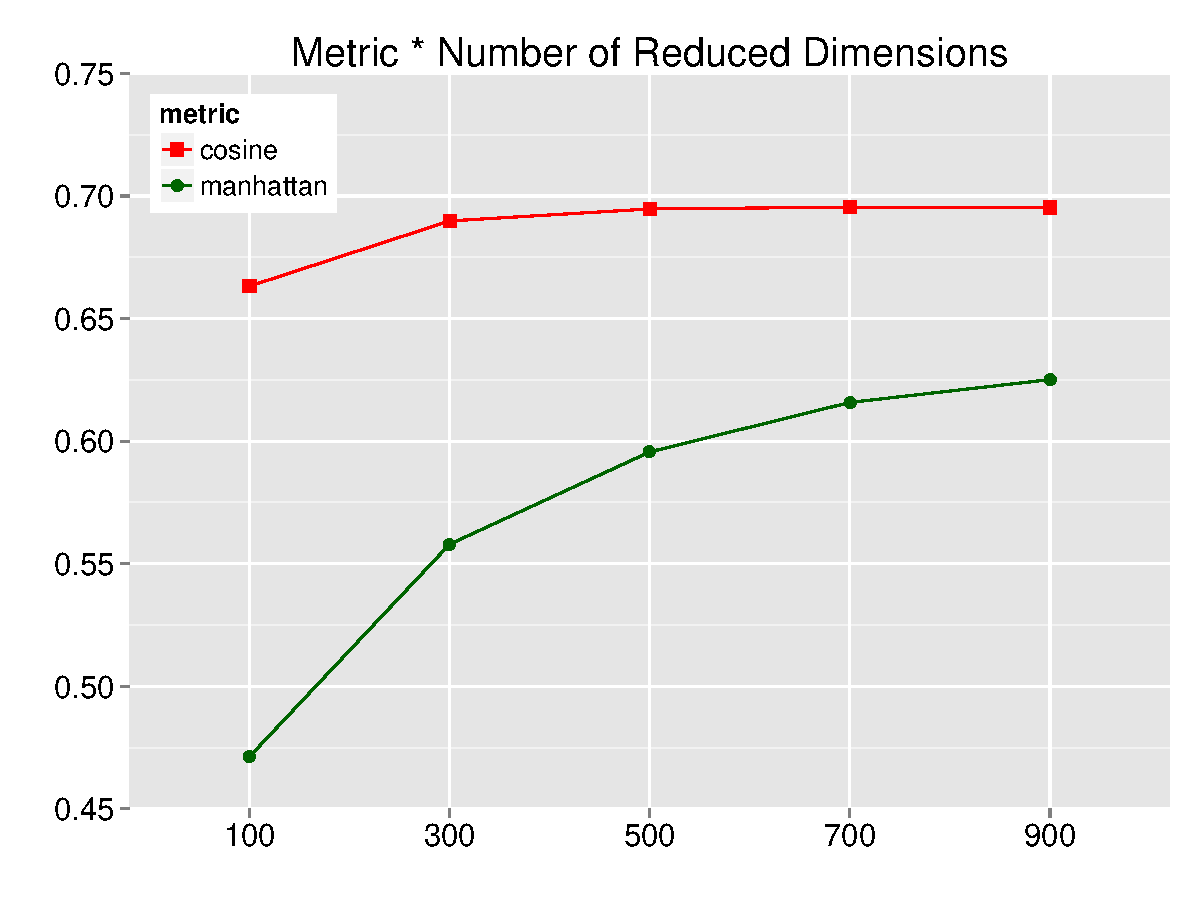
\includegraphics[scale=0.30]{img/lapesa_rg_main_metric_n-dim} &
    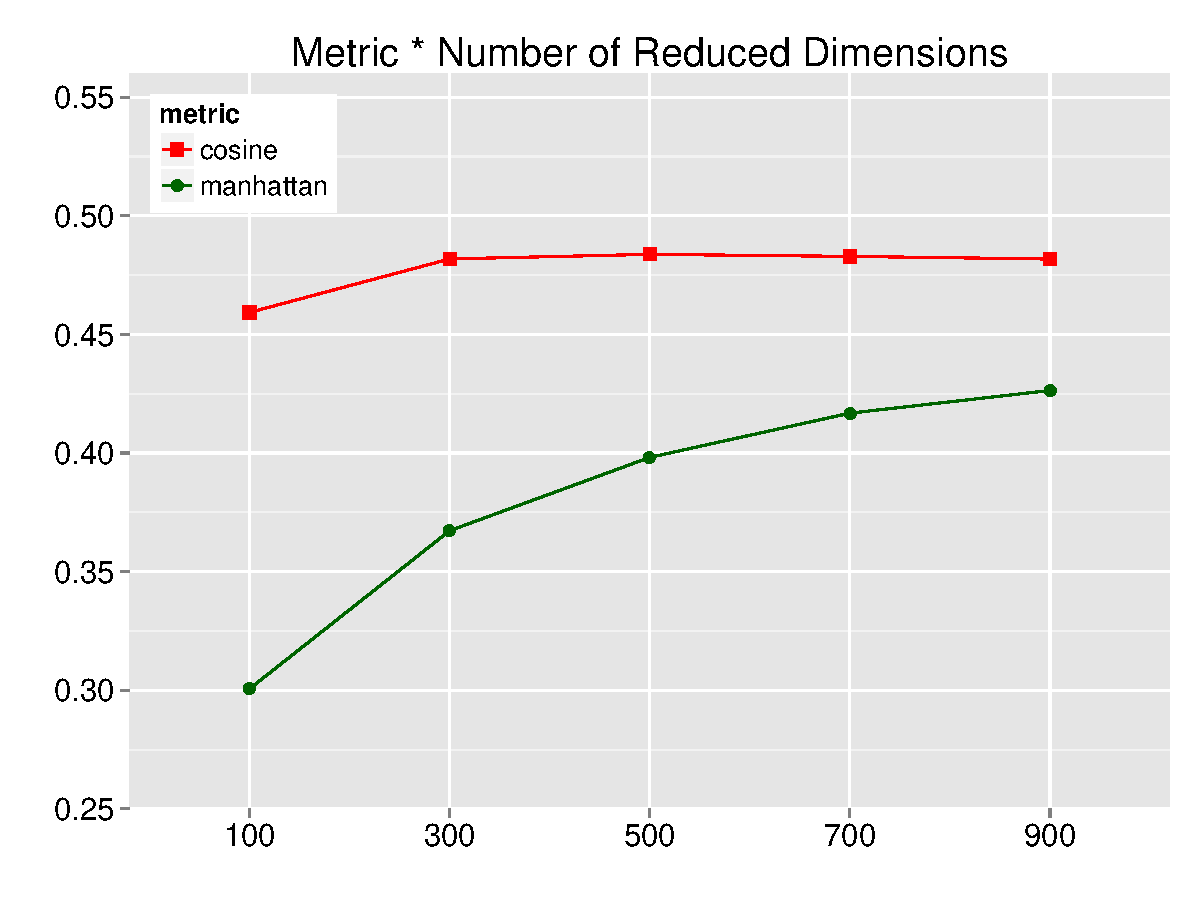
\includegraphics[scale=0.30]{img/lapesa_ws_main_metric_n-dim} \\
    \secondary{Rubenstein \& Goodenough} &
    \secondary{WordSim-353}
  \end{tabular}
\end{frame}

\begin{frame}
  \frametitle{Similarity ratings: Number of Skipped Dimensions}
  \framesubtitle{Partial effect displays \citep{Fox:03}} 

  \centering
  \gap[1]\hspace*{-1cm}%
  \begin{tabular}{c@{}c}
    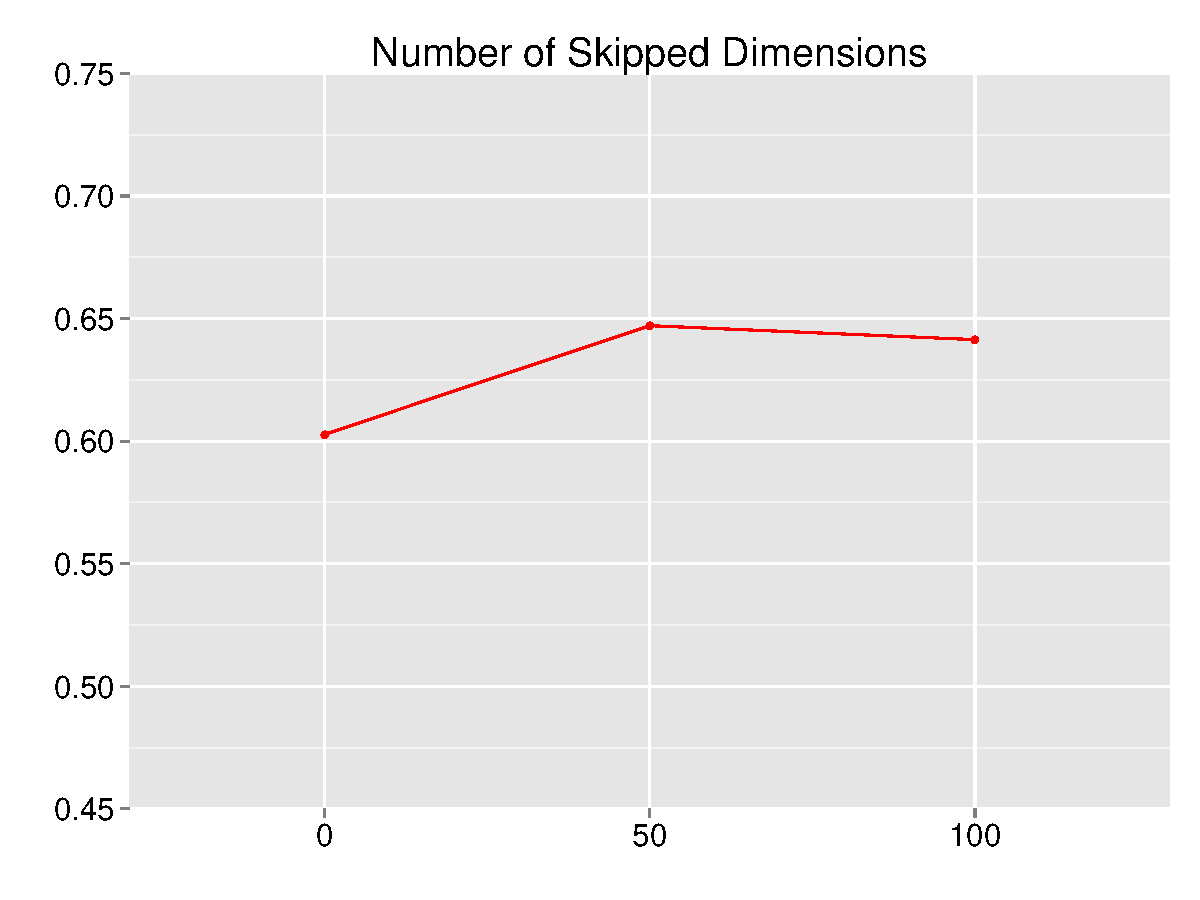
\includegraphics[scale=0.30]{img/lapesa_rg_main_dimskip} &
    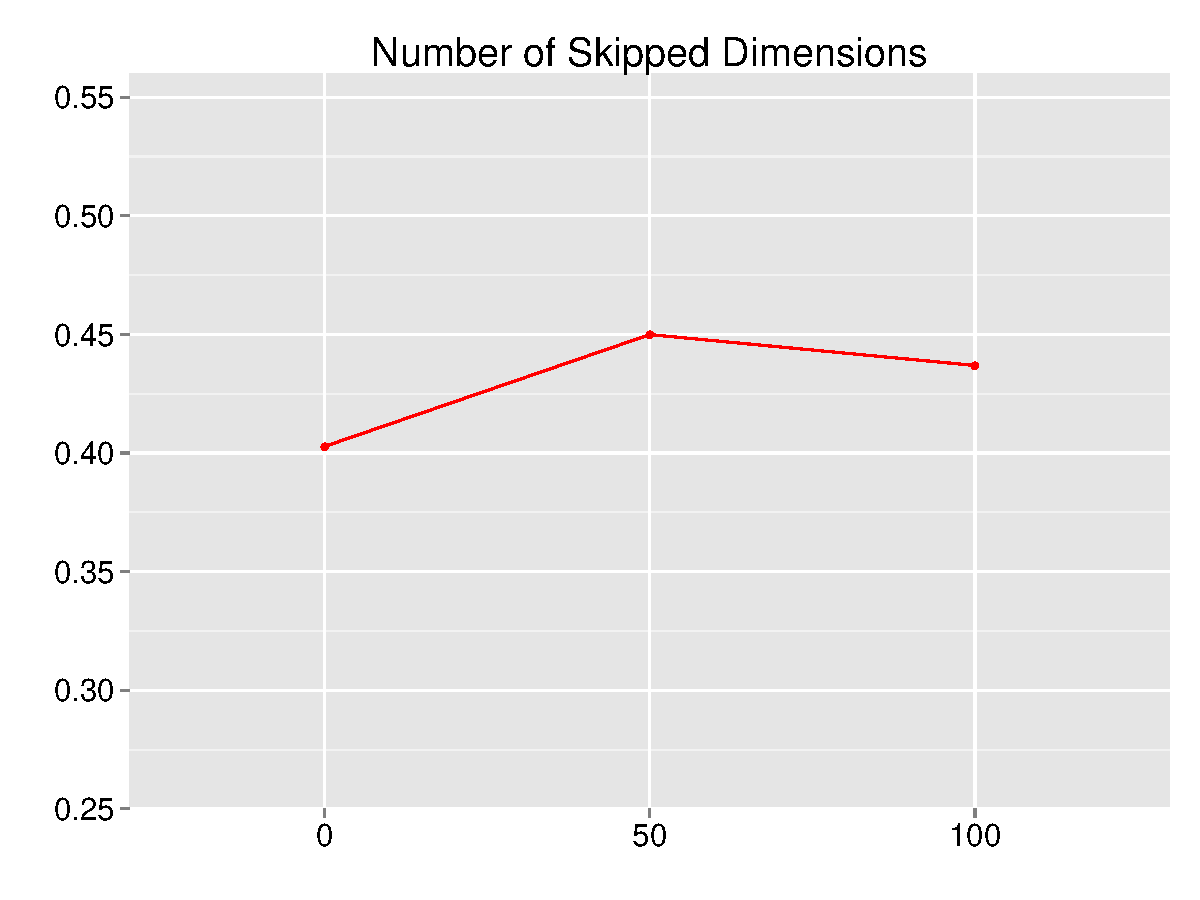
\includegraphics[scale=0.30]{img/lapesa_ws_main_dimskip} \\
    \secondary{Rubenstein \& Goodenough} &
    \secondary{WordSim-353}
  \end{tabular}
\end{frame}

\begin{frame}
  \frametitle{Similarity ratings: Window Size, Transformation}
  \framesubtitle{Partial effect displays \citep{Fox:03}} 

  \centering
  \gap[1]\hspace*{-1cm}%
  \begin{tabular}{c@{}c}
    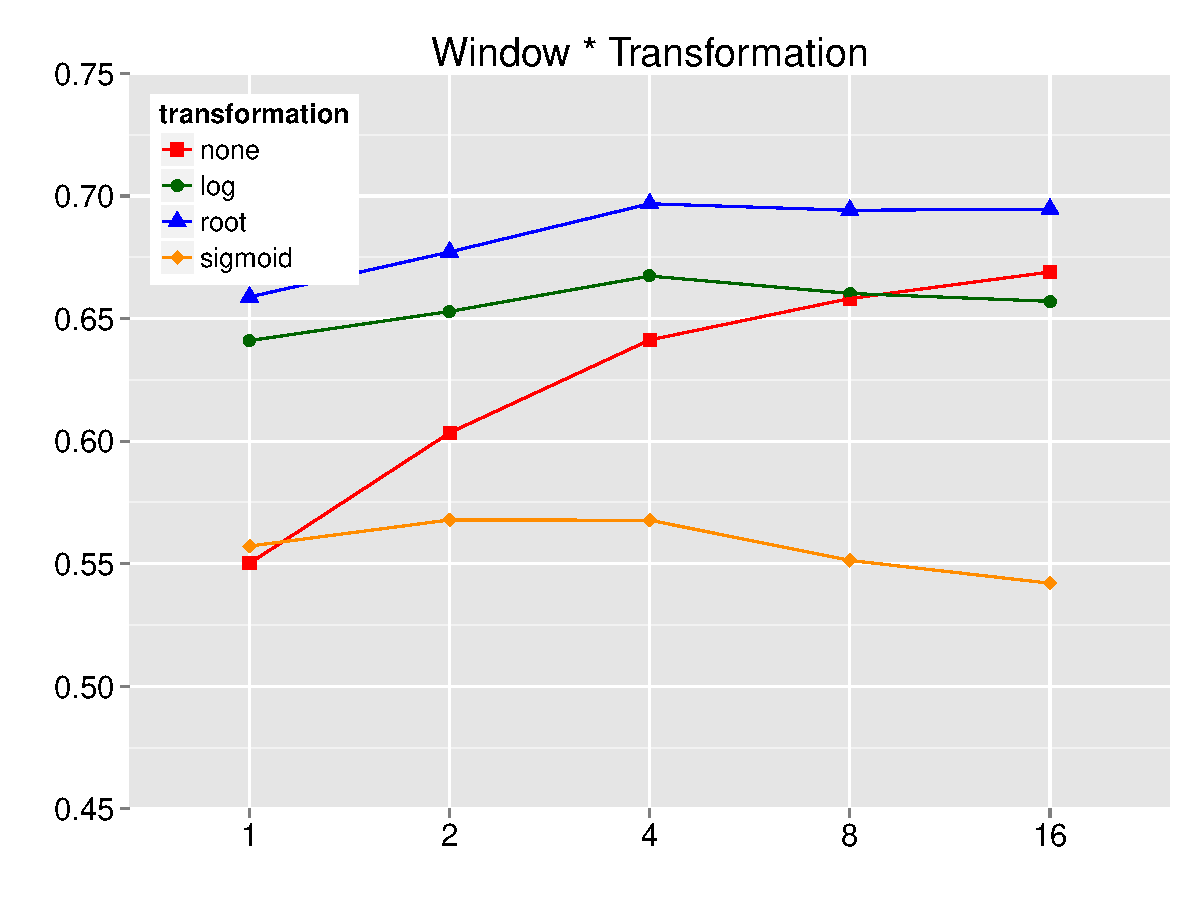
\includegraphics[scale=0.30]{img/lapesa_rg_main_window_transformation} &
    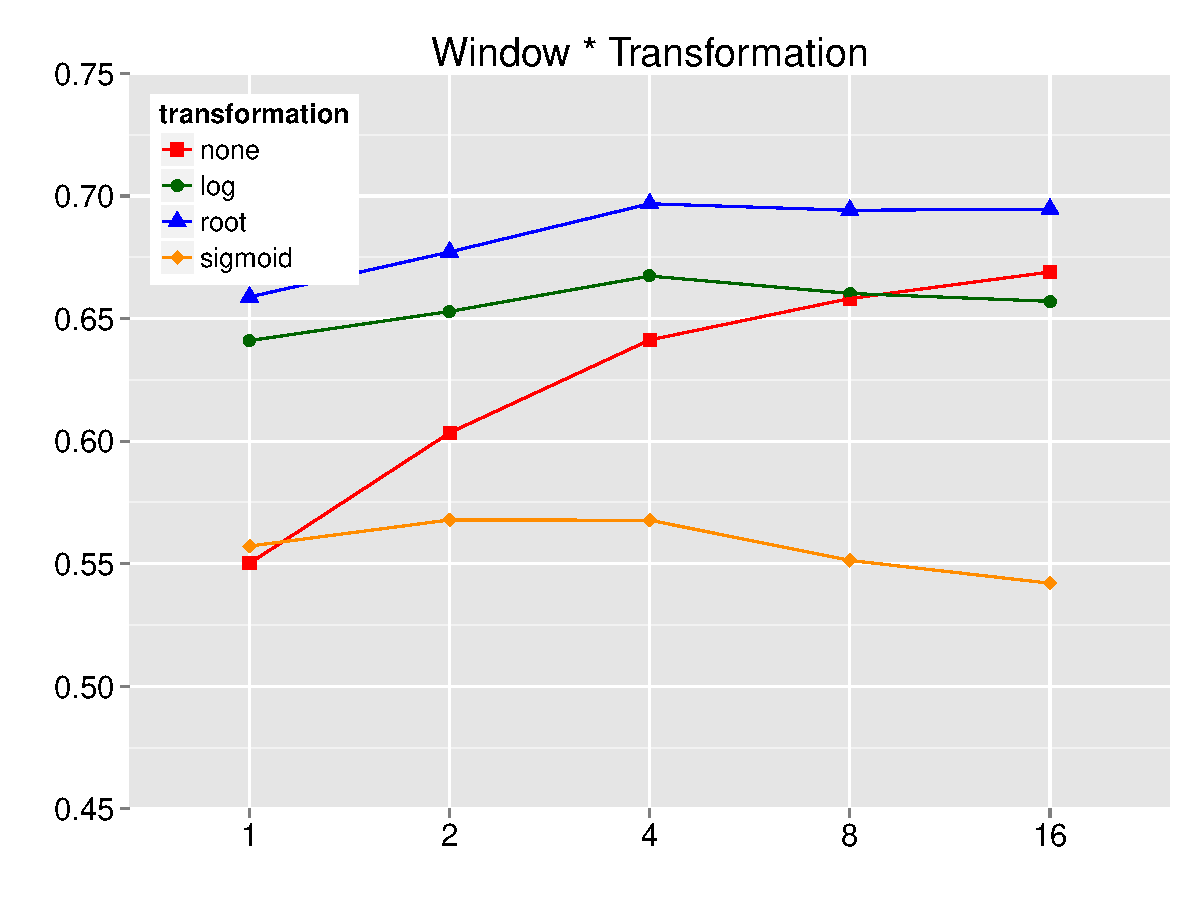
\includegraphics[scale=0.30]{img/lapesa_rg_main_window_transformation} \\
    \secondary{Rubenstein \& Goodenough} &
    \secondary{WordSim-353}
  \end{tabular}
\end{frame}

\begin{frame}
  \frametitle{Summing up: Ratings}
  \begin{exampleblock}{Ratings: best setting}
    \begin{itemize}\footnotesize
    \item Corpus: wacky
    \item Window: undirected, 4 words 
    \item Feature selection: top 20000/50000 dimensions, based on frequency
    \item Score * Transformation: simple-ll * log
    \item Dimensionality Reduction: 300 latent dimensions, skipping the first 50
    \item Distance Metric: cosine
    \item Index of Distributional Relatedness: neighbor rank
    \end{itemize}
  \end{exampleblock}  
\end{frame}


\begin{frame}
  \frametitle{DSMs and semantic clustering}
  \framesubtitle{Introducing the task}

  \ungap[1.5]
  \begin{columns}
    \begin{column}{0.5 \textwidth}
      \begin{exampleblock}{Almuhareb \& Poesio}
        \textbf{402 nouns, 21 classes} \\
        \textit{day} $\Longrightarrow$ \textsc{time}   \\
        \textit{kiwi} $\Longrightarrow$ \textsc{fruit}  \\
        \textit{kitten} $\Longrightarrow$ \textsc{animal} \\
        \textit{volleyball} $\Longrightarrow$ \textsc{game}
      \end{exampleblock}
      \begin{exampleblock}{ESSLLI categorization task}
        \textbf{44 nouns, 6 classes} \\
        \textit{potato} $\Longrightarrow$ \textsc{green}  \\
        \textit{hammer} $\Longrightarrow$ \textsc{tool}  \\
        \textit{car} $\Longrightarrow$ \textsc{vehicle} \\
        \textit{peacock} $\Longrightarrow$ \textsc{bird}     
      \end{exampleblock}
    \end{column}
    \begin{column}{0.5 \textwidth}
      \begin{exampleblock}{BATTIG set}
        \textbf{82 nouns, 10 classes} \\
        \textit{chicken} $\Longrightarrow$ \textsc{bird}   \\
        \textit{bear} $\Longrightarrow$ \textsc{land\_mammal}  \\
        \textit{pot} $\Longrightarrow$ \textsc{kitchenware} \\
        \textit{oak} $\Longrightarrow$ \textsc{tree} 
      \end{exampleblock}
      \begin{exampleblock}{MITCHELL set}
        \textbf{60 nouns, 12 classes} \\
        \textit{ant} $\Longrightarrow$ \textsc{insect}   \\
        \textit{carrot} $\Longrightarrow$ \textsc{vegetable}  \\
        \textit{train} $\Longrightarrow$ \textsc{vehicle} \\
        \textit{cat} $\Longrightarrow$ \textsc{animal}
      \end{exampleblock}
    \end{column}
  \end{columns}
\end{frame}

\begin{frame}
  \frametitle{DSMs and semantic clustering}
  \framesubtitle{Introducing the task}

  \begin{itemize}
  \item A \textbf{categorization} task
  \item If distributional representations approximate human conceptual representations, we expect word categorization based on distributional features to produce concept clusters similar to those in the gold standard datasets
  \item Performance: \textbf{cluster purity}
    \begin{itemize}
    \item classification accuracy for optimal cluster labelling
    \item percentage of nouns that belong to the majority category within their cluster 
    \end{itemize}
  \item<2-> \secondary{Partitioning around medoids} \citep{Kaufman:Rousseeuw:90}
    \begin{itemize}
    \item implemented as \texttt{pam()} in R standard library
    \item direct comparison \so equal to or even better than CLUTO
    \item works with arbitrary dissimilarity matrix
    \end{itemize}
  \end{itemize}
\end{frame}

\begin{frame}
  \frametitle{Semantic clustering: performance}
  \framesubtitle{Overview: unreduced versus reduced experiments}

  \begin{center}
    \begin{tabular}{|l|c|c|c|c|c|c|}
      \hline
      \multirow{2}{*}{Dataset}  & \multicolumn{3}{c|}{Unreduced} &  \multicolumn{3}{c|}{Reduced} \\  \cline{2-7}
      & Min & Max & Mean & Min & Max & Mean \\
      \hline      
      AP & 0.15 & 0.73 & 0.56 & 0.13 & \primary{0.76} & 0.54 \\  
      BATTIG & 0.28 & \primary{0.99} & 0.77 & 0.23 & \primary{0.99} & 0.78  \\  
      ESSLLI & 0.32 & 0.93 & 0.72 & 0.32 & \primary{0.98} & 0.72  \\    
      MITCHELL & 0.26 & \primary{0.97} & 0.68 & 0.27 & \primary{0.97} & 0.69 \\
      \hline
    \end{tabular}

    \gap[1]
    \secondary{Semantic clustering: summary of performance (purity)} 
  \end{center}
\end{frame}

\begin{frame}
  \frametitle{Semantic clustering: parameters and explained variance}
  \framesubtitle{Feature ablation  (model $R^{2}$ -- AP: 82\%;  BATTIG: 77\%; ESSLLI  58\%; MITCHELL 73\%)}

  \centering
  \hspace*{-10pt}
  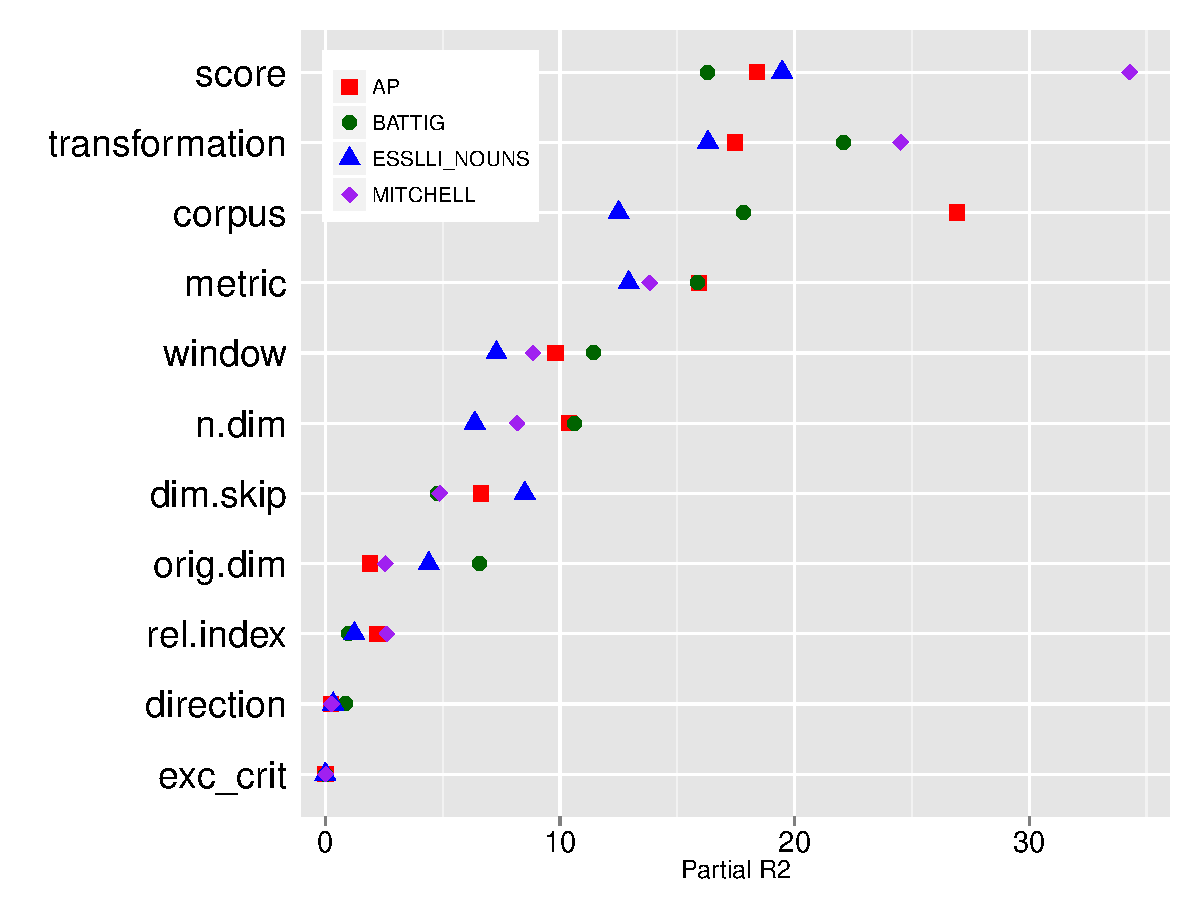
\includegraphics[scale=0.45]{img/lapesa_clustering_main_r2_reduced}
\end{frame}

\begin{frame}
  \frametitle{Semantic clustering: interactions}
  \framesubtitle{Reduced setting ($R^{2} > 0.5$)}
  
  \begin{center}\small
    \begin{tabular}{lrrrrr}
      Interaction & Df & AP & BATTIG & ESSLLI & MITCHELL \\ \hline
      
      \primary{score:transformation} & 18 &  7.10  & 7.95 & 7.56  &  11.42   \\ 
      \primary{window:metric} & 4 &  2.22   & 1.26 & 2.97  & 2.72    \\
      \primary{metric:n.dim} & 4 &   3.29    & 3.16 &  2.03 &  0.58   \\   
      \primary{metric:dim.skip} & 2 &   2.25   & 1.54 & 2.77  & 	 0.86  \\   
      \primary{window:transformation} & 12 &  2.00  & 2.95 & 0.88  &   2.66 \\ 

      corpus:metric & 2 &  1.42  & 2.91 & 2.79   & 1.11      \\ 
      corpus:window & 8 &   2.36   & 1.18 & 1.49  &    1.23   \\ 
      score:dim.skip & 12 &  0.56 & 1.15 &   0.99 &   1.39 \\ 
      window:score & 24 &  0.74   & 0.77 &  0.54  &  0.65  \\  
      %% metric:orig.dim & 4 &    -  & 1.20 &  0.67  &  0.92  \\ 
      %% transformation:dim.skip & 6 &   -   & 1.17 &  0.85  &  1.39    \\   
    \end{tabular}

    \gap[1]\normalsize
    \secondary{Clustering datasets: interactions, $R^2$} 
  \end{center}
\end{frame}

\begin{frame}
  \frametitle{Semantic clustering: Score, Transformation}
  \framesubtitle{Partial effect displays \citep{Fox:03}} 

  \centering
  \gap[1]\hspace*{-1cm}%
  \begin{tabular}{c@{}c}
    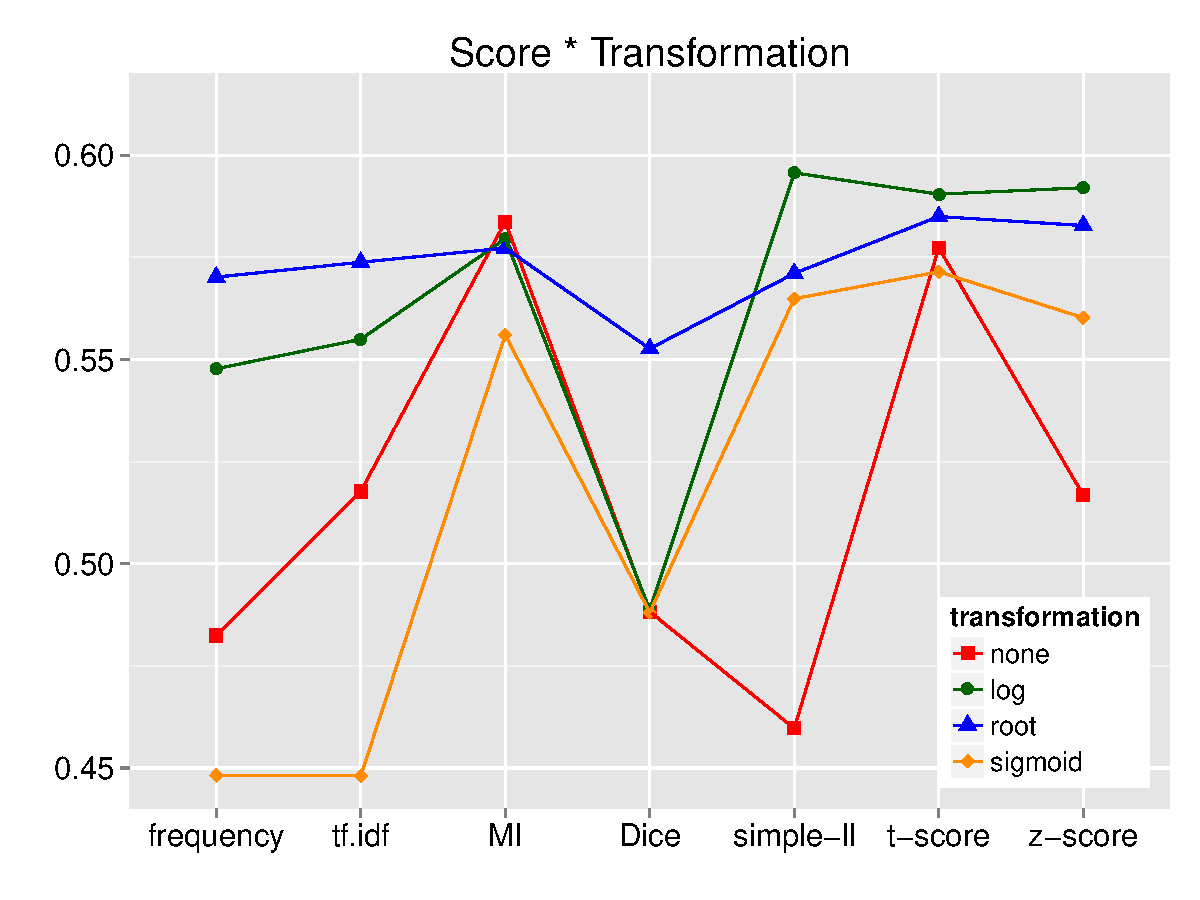
\includegraphics[scale=0.30]{img/lapesa_ap_main_score_transformation} &
    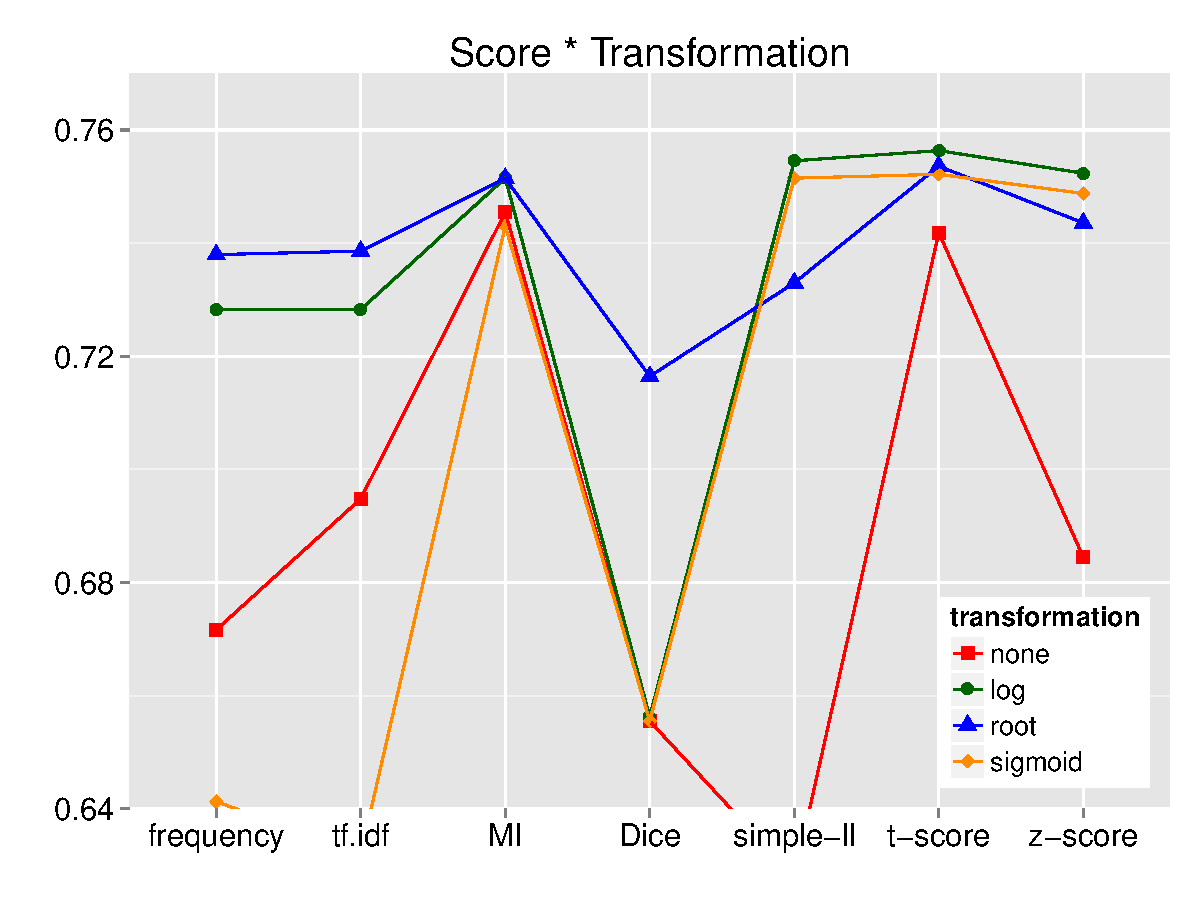
\includegraphics[scale=0.30]{img/lapesa_esslli_main_score_transformation} \\
    \secondary{Almuhareb \& Poesio} &
    \secondary{ESSLLI 2008}
  \end{tabular}
\end{frame}

\begin{frame}
  \frametitle{Semantic clustering: Corpus}
  \framesubtitle{Partial effect displays \citep{Fox:03}} 

  \centering
  \gap[1]\hspace*{-1cm}%
  \begin{tabular}{c@{}c}
    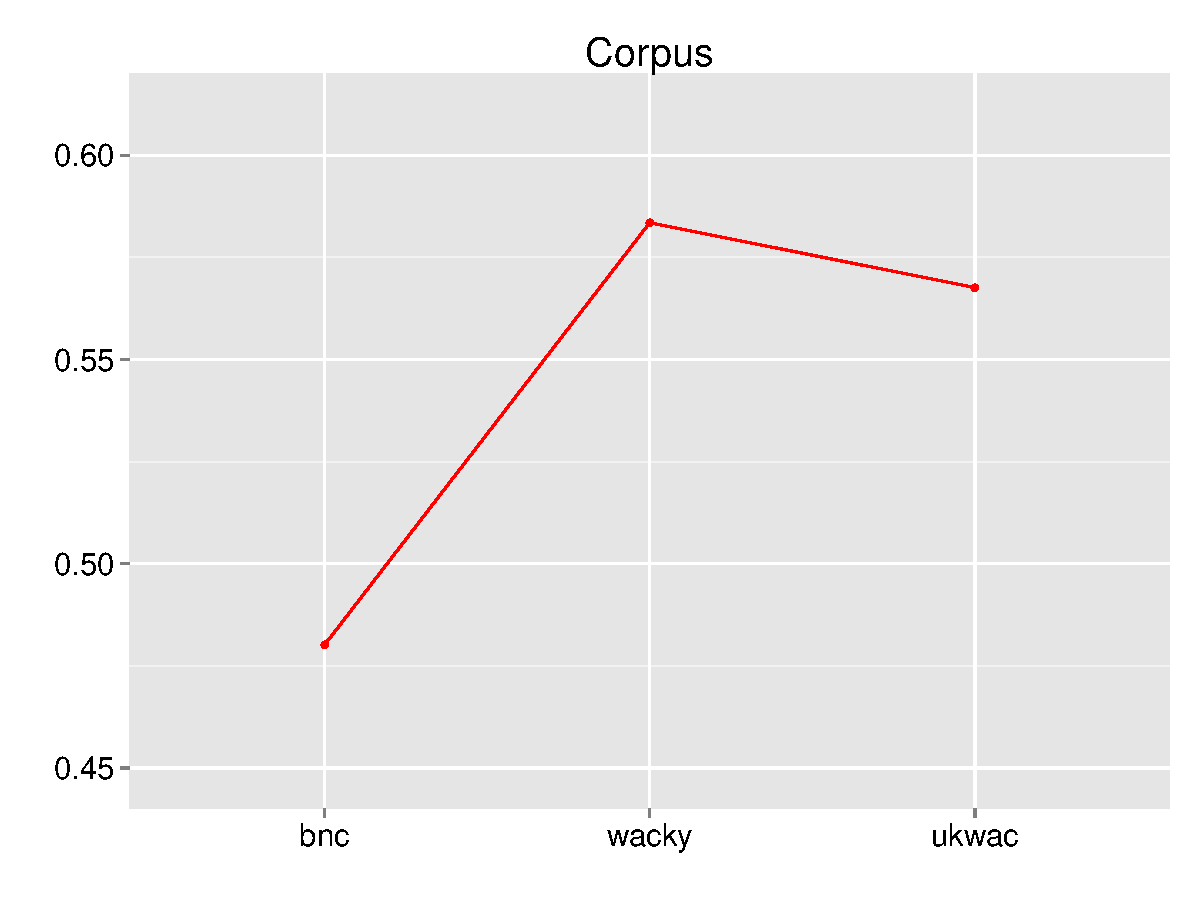
\includegraphics[scale=0.30]{img/lapesa_ap_main_corpus} &
    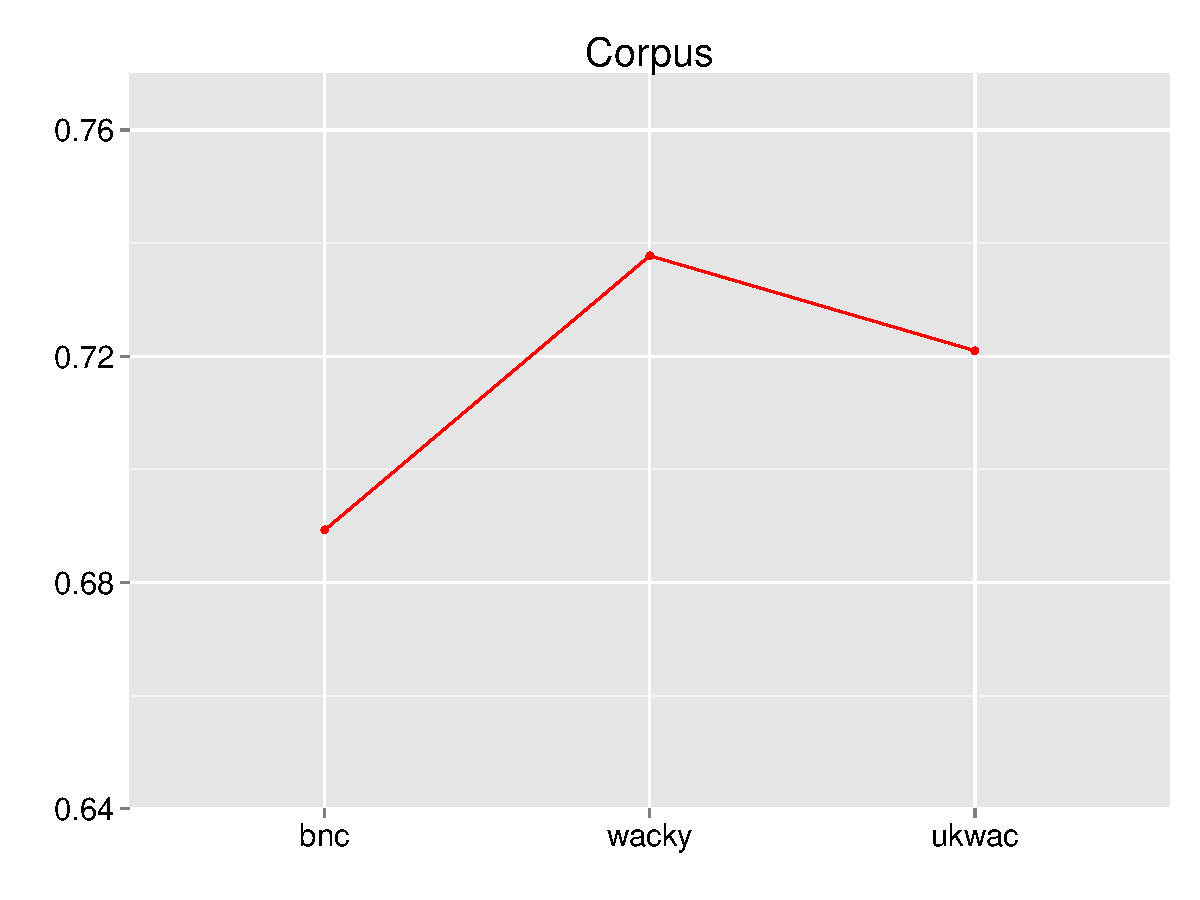
\includegraphics[scale=0.30]{img/lapesa_esslli_main_corpus} \\
    \secondary{Almuhareb \& Poesio} &
    \secondary{ESSLLI 2008}
  \end{tabular}
\end{frame}

\begin{frame}
  \frametitle{Semantic clustering: Window Size, Metric}
  \framesubtitle{Partial effect displays \citep{Fox:03}} 

  \centering
  \gap[1]\hspace*{-1cm}%
  \begin{tabular}{c@{}c}
    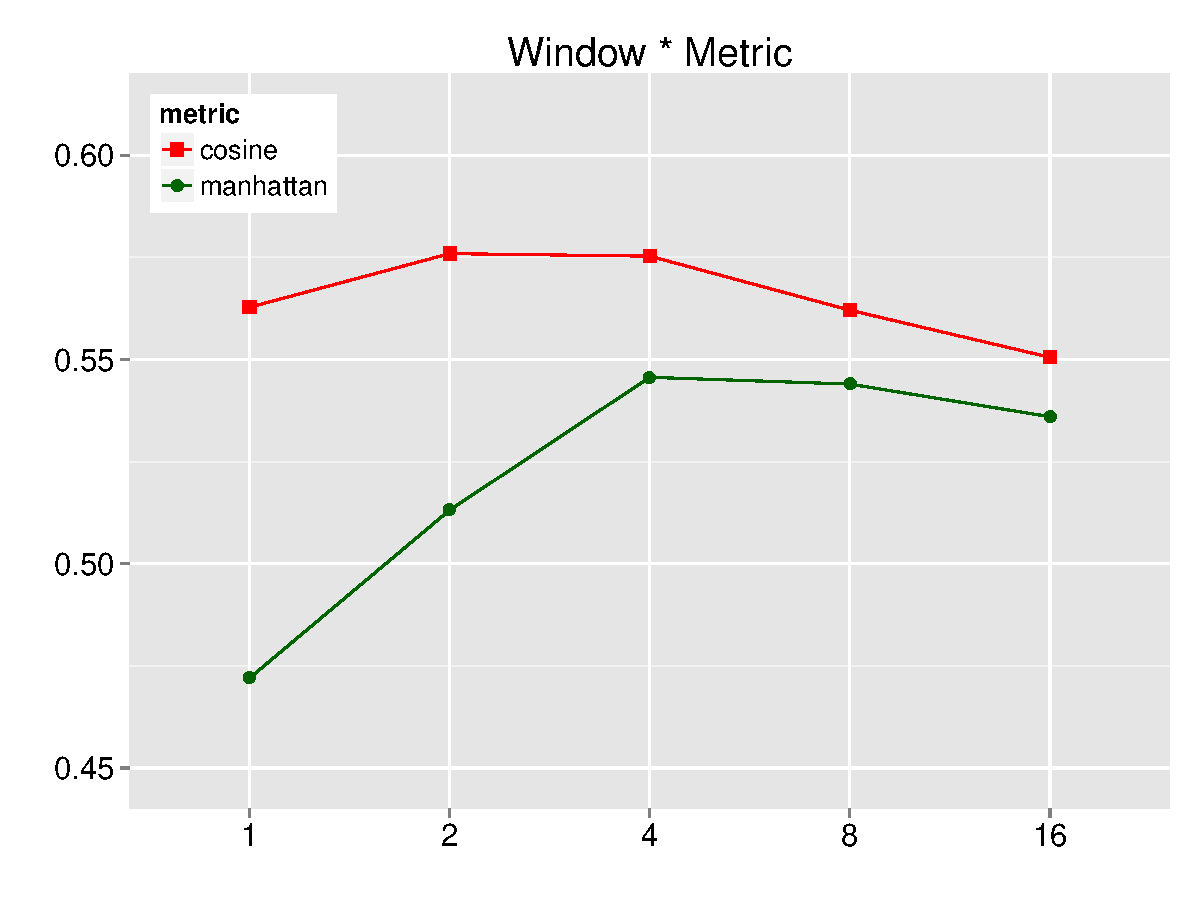
\includegraphics[scale=0.30]{img/lapesa_ap_main_window_metric} &
    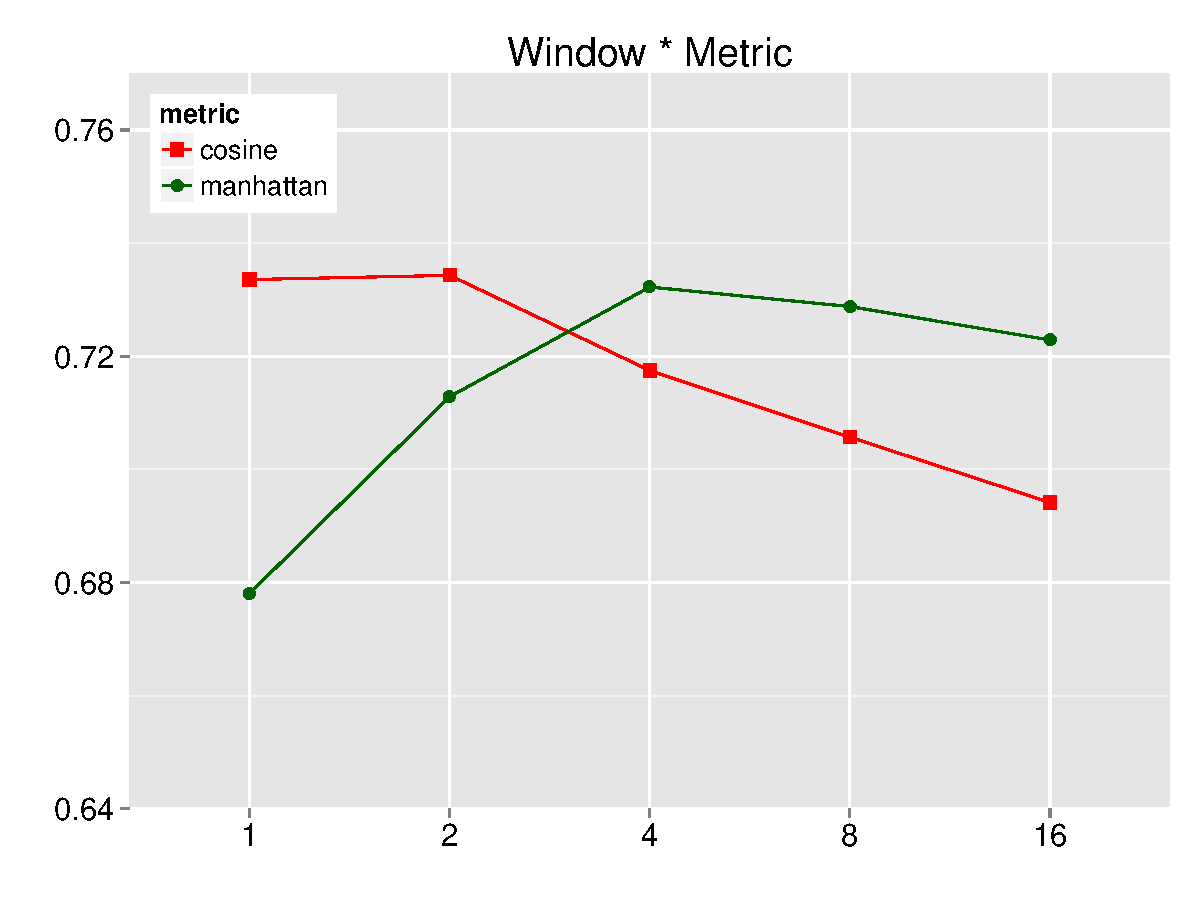
\includegraphics[scale=0.30]{img/lapesa_esslli_main_window_metric} \\
    \secondary{Almuhareb \& Poesio} &
    \secondary{ESSLLI 2008}
  \end{tabular}
\end{frame}

\begin{frame}
  \frametitle{Semantic clustering: Metric, Number of Latent Dimensions}
  \framesubtitle{Partial effect displays \citep{Fox:03}} 

  \centering
  \gap[1]\hspace*{-1cm}%
  \begin{tabular}{c@{}c}
    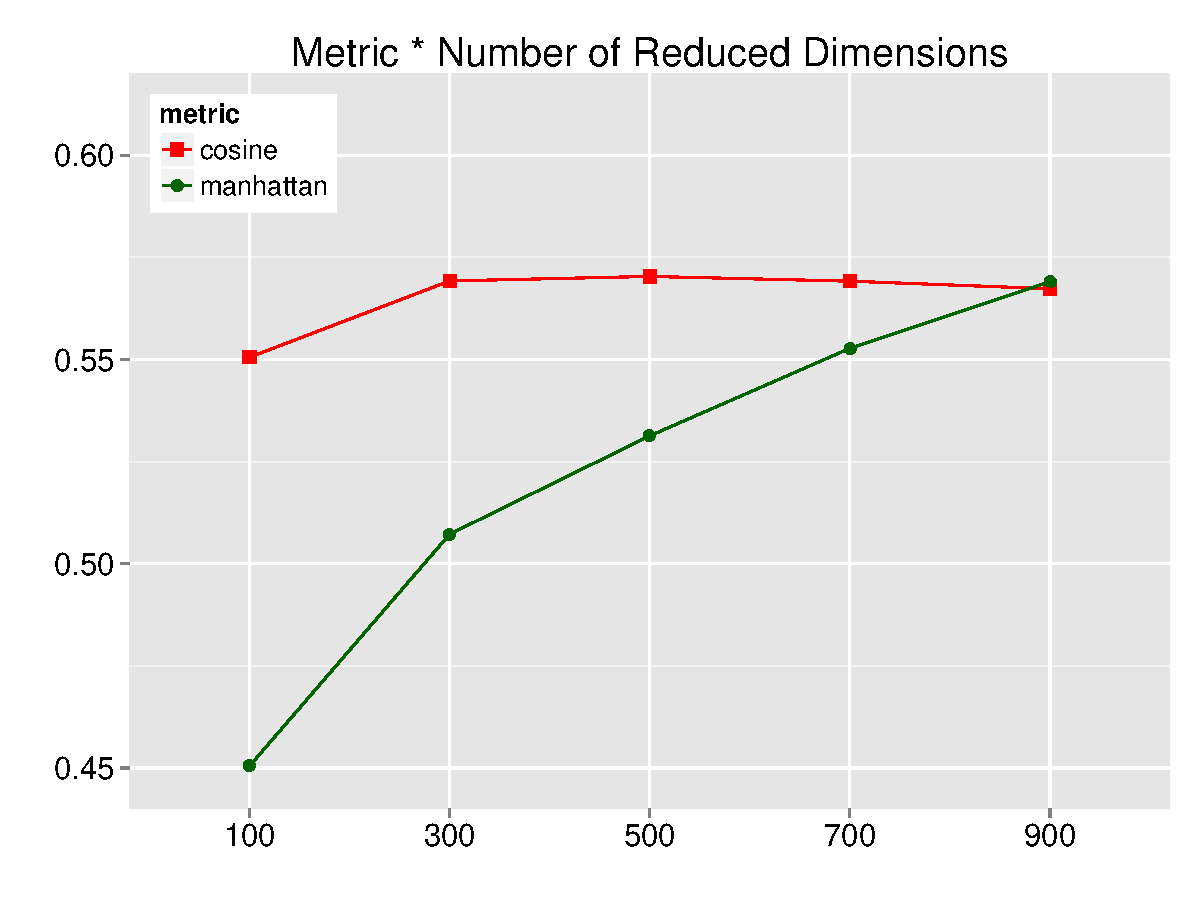
\includegraphics[scale=0.30]{img/lapesa_ap_main_metric_n-dim} &
    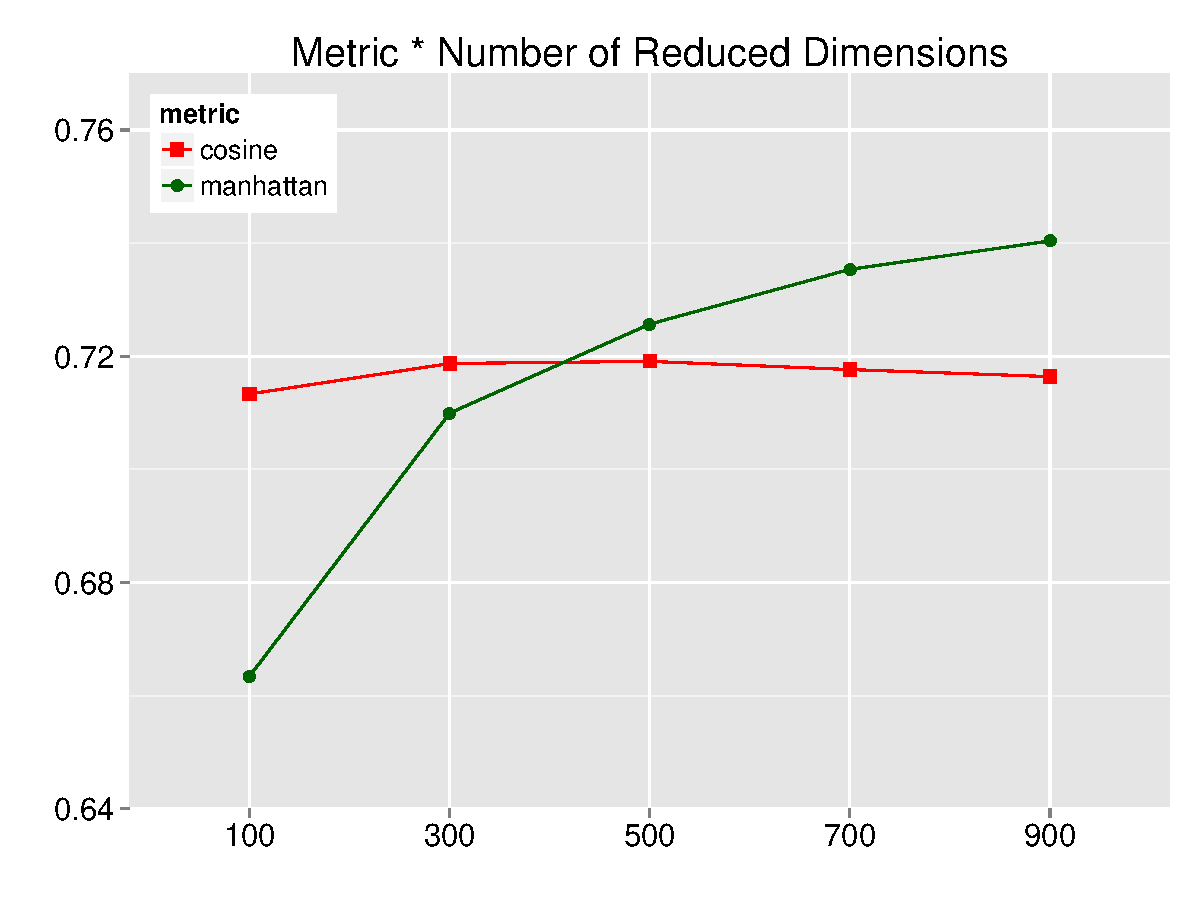
\includegraphics[scale=0.30]{img/lapesa_esslli_main_metric_n-dim} \\
    \secondary{Almuhareb \& Poesio} &
    \secondary{ESSLLI 2008}
  \end{tabular}
\end{frame}

\begin{frame}
  \frametitle{Semantic clustering: Number of Skipped Dimensions}
  \framesubtitle{Partial effect displays \citep{Fox:03}} 

  \centering
  \gap[1]\hspace*{-1cm}%
  \begin{tabular}{c@{}c}
    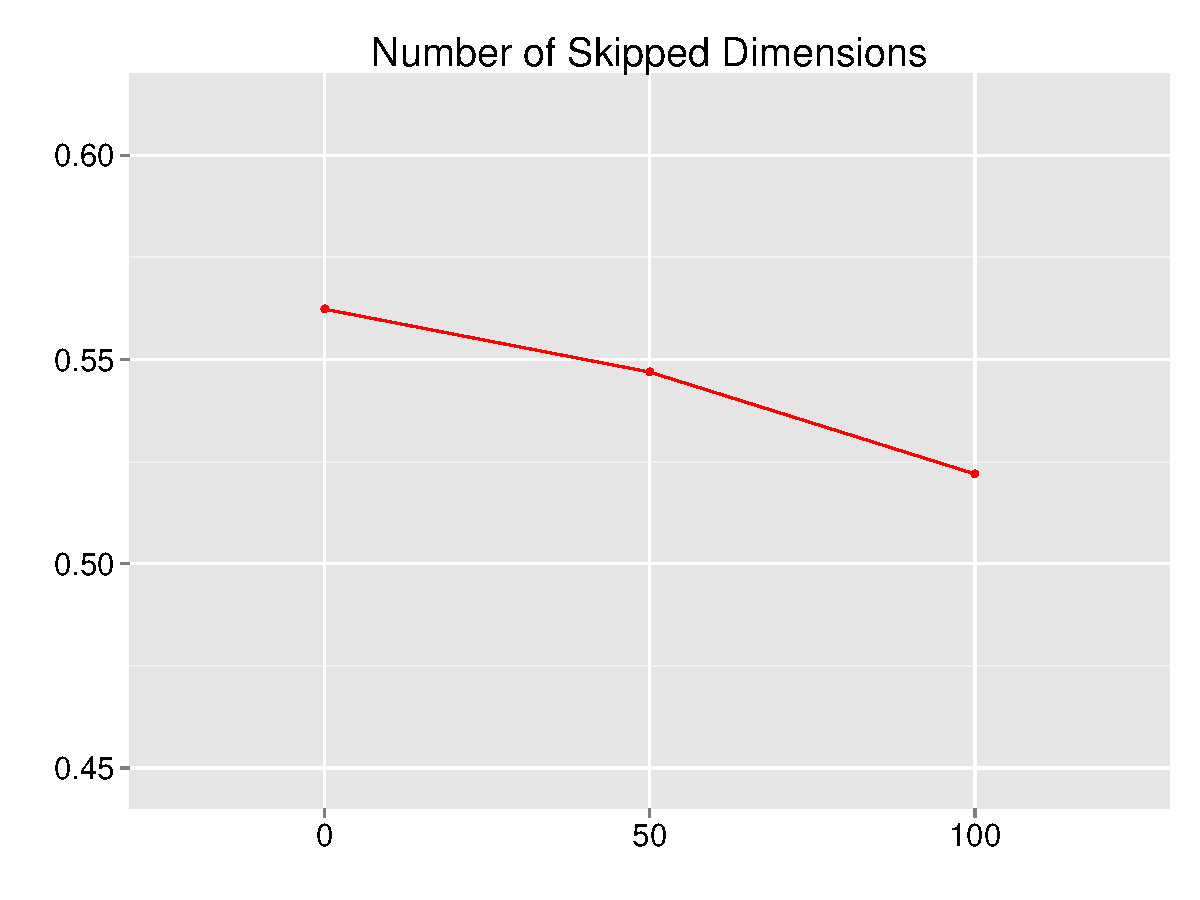
\includegraphics[scale=0.30]{img/lapesa_ap_main_dimskip} &
    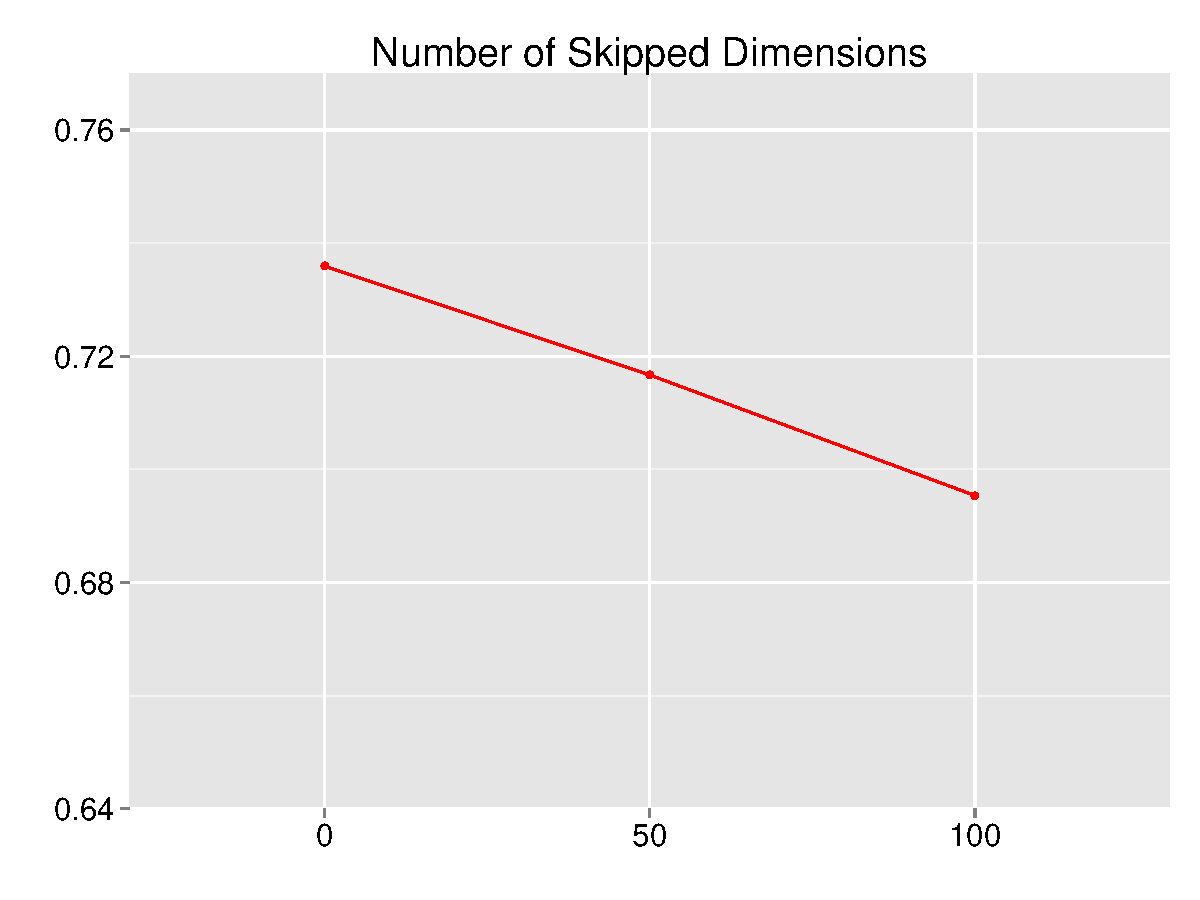
\includegraphics[scale=0.30]{img/lapesa_esslli_main_dimskip} \\
    \secondary{Almuhareb \& Poesio} &
    \secondary{ESSLLI 2008}
  \end{tabular}
\end{frame}

\begin{frame}
  \frametitle{Semantic clustering: Relatedness Index}
  \framesubtitle{Partial effect displays \citep{Fox:03}} 

  \centering
  \gap[1]\hspace*{-1cm}%
  \begin{tabular}{c@{}c}
    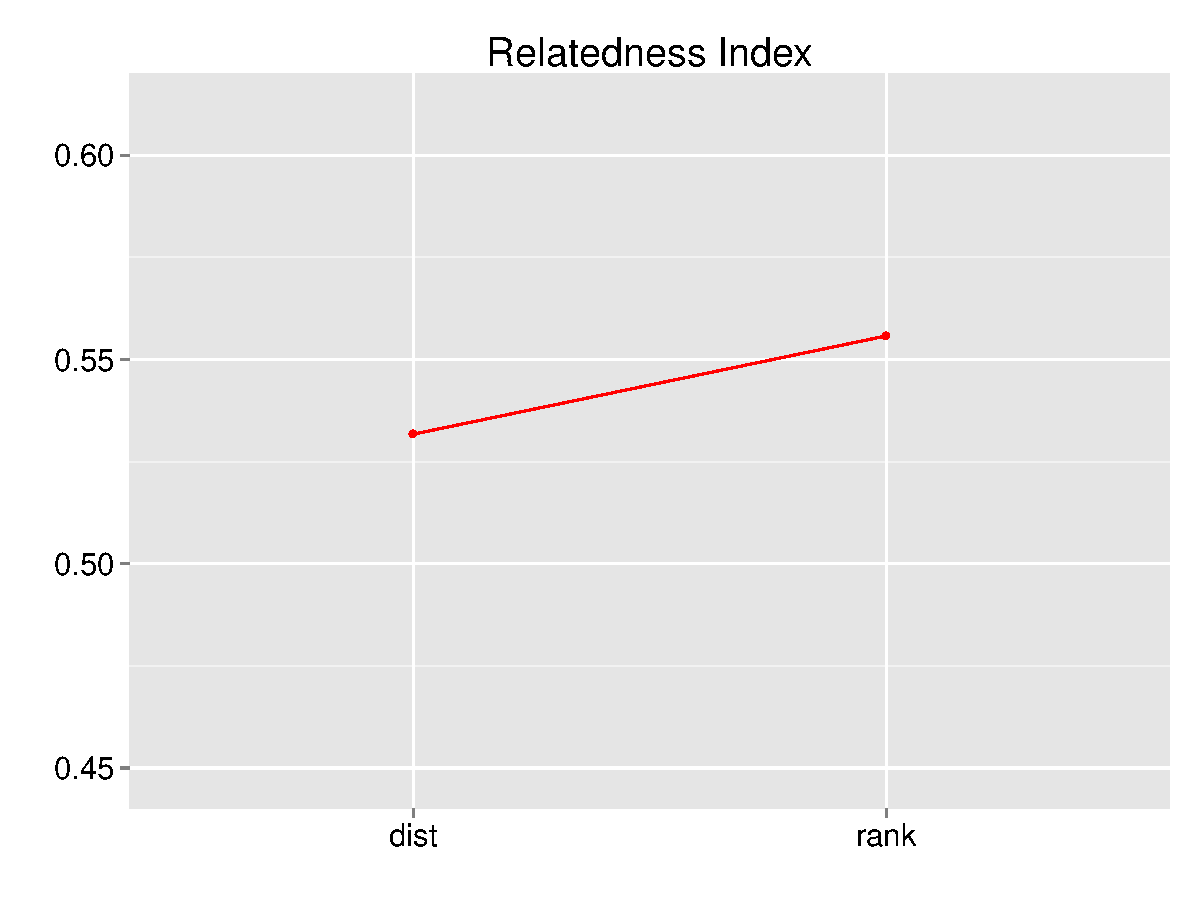
\includegraphics[scale=0.30]{img/lapesa_ap_main_relindex} &
    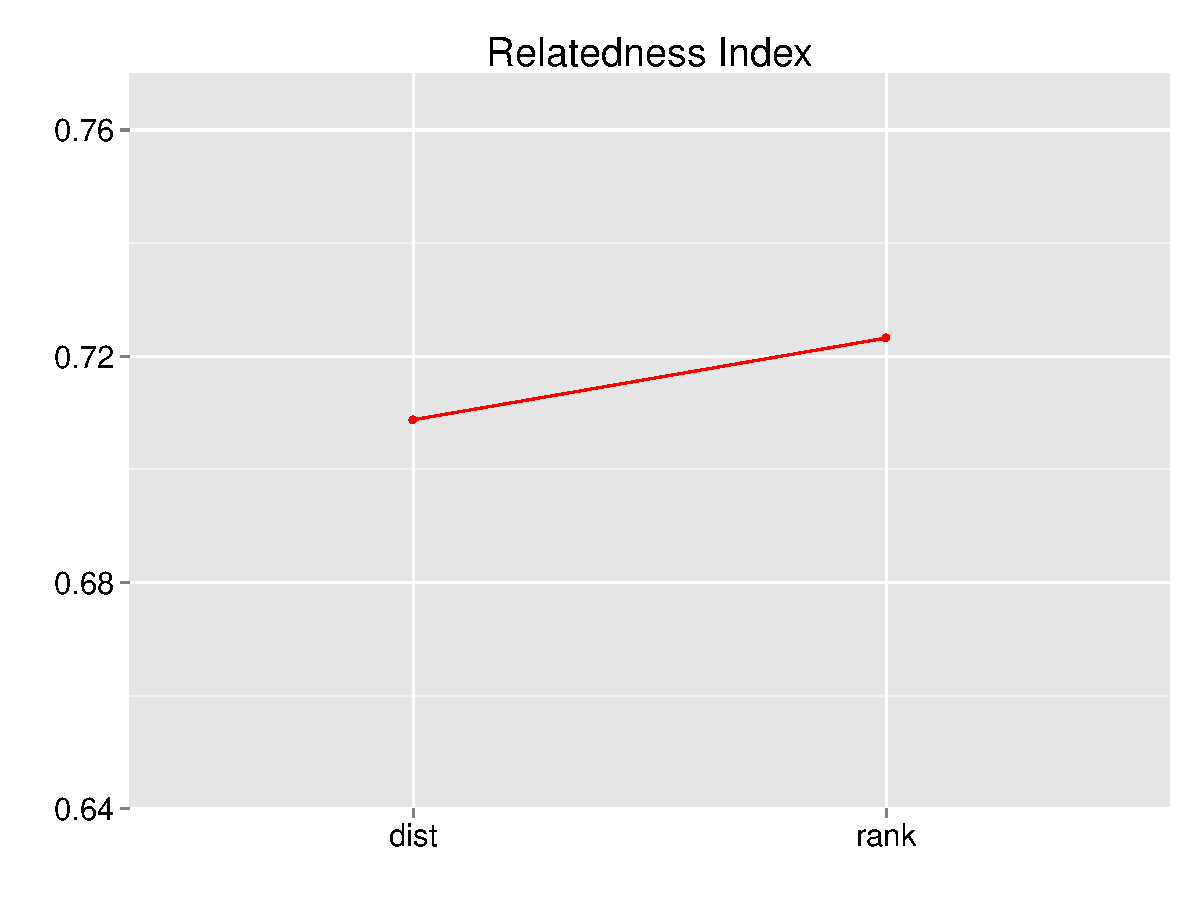
\includegraphics[scale=0.30]{img/lapesa_esslli_main_relindex} \\
    \secondary{Almuhareb \& Poesio} &
    \secondary{ESSLLI 2008}
  \end{tabular}
\end{frame}

\begin{frame}
  \frametitle{Semantic clustering: Number of Feature Dimensions}
  \framesubtitle{Partial effect displays \citep{Fox:03}} 

  \centering
  \gap[1]\hspace*{-1cm}%
  \begin{tabular}{c@{}c}
    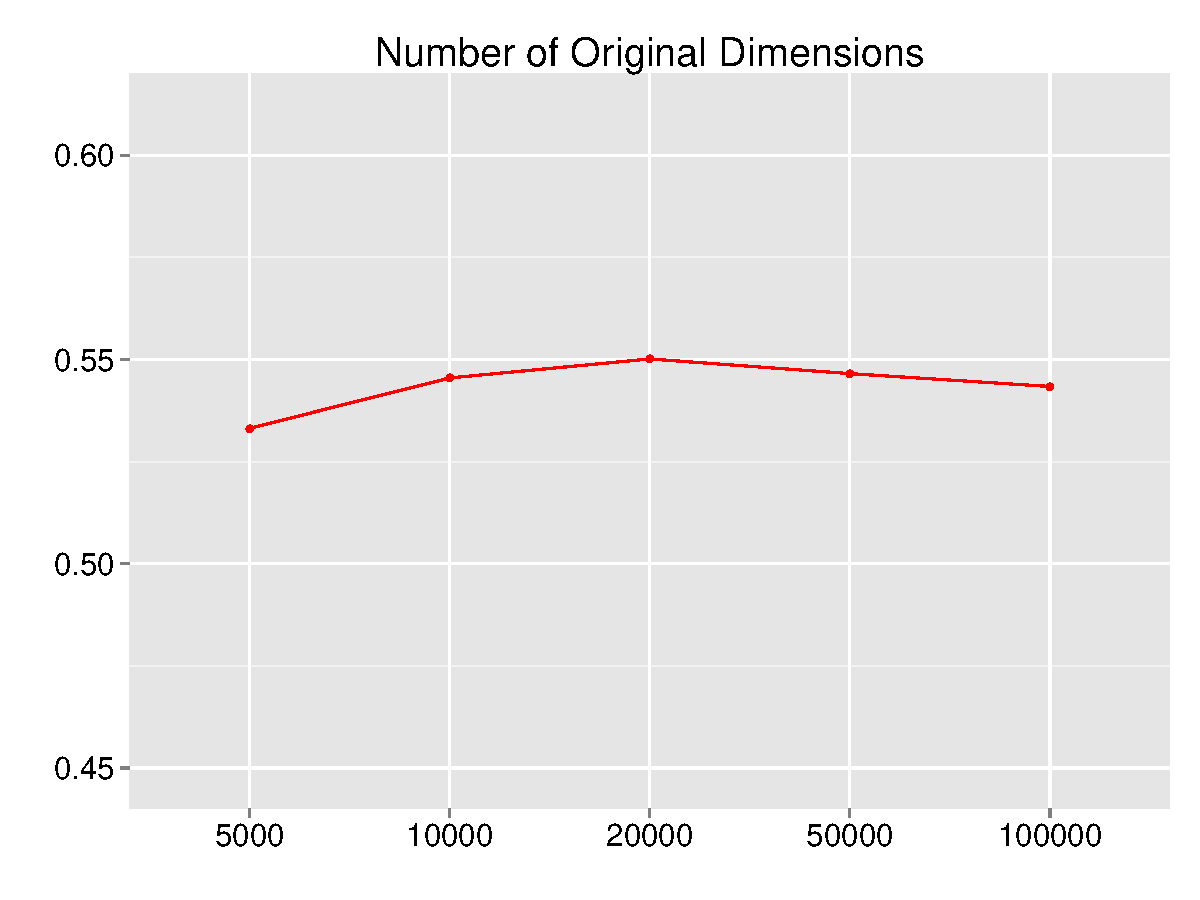
\includegraphics[scale=0.30]{img/lapesa_ap_main_origdim} &
    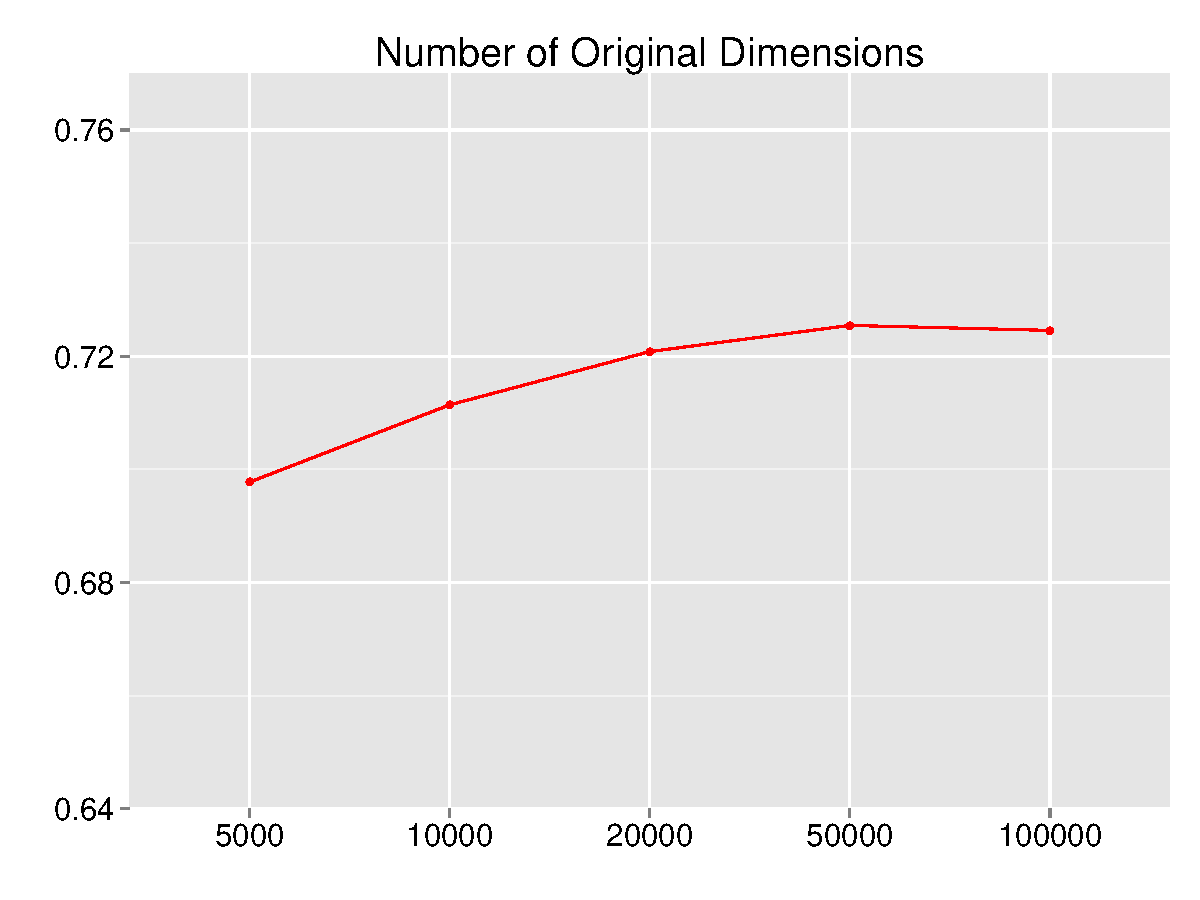
\includegraphics[scale=0.30]{img/lapesa_esslli_main_origdim} \\
    \secondary{Almuhareb \& Poesio} &
    \secondary{ESSLLI 2008}
  \end{tabular}
\end{frame}

\begin{frame}
  \frametitle{Summing up: Semantic Clustering}
  \begin{exampleblock}{Clustering: best setting}
    \begin{itemize}
    \item Corpus: wacky
    \item Window: undirected, 4 words 
    \item Feature selection: top 50000 dimensions, based on frequency
    \item Score * Transformation: simple-ll * log (or t-score * log)
    \item Dimensionality Reduction: 300/500 latent dimensions,\\ no skipping necessary
    \item Distance Metric: cosine
    \item Index of Distributional Relatedness: neighbor rank
    \end{itemize}
  \end{exampleblock}   
\end{frame}


%%%%%%%%%%%%%%%%%%%%%%%%%%%%%%%%%%%%%%%%%%
\subsection{Summary \& conclusion}

\begin{frame}
  \frametitle{Does our evaluation methodology work?}

  \begin{enumerate}
  \item What are the most explanatory parameters?
  \item By inspecting the effect plots, we identified best settings for every dataset: what is the performance of such best settings? Are they close to the best runs in the experiment? 
  \item Is it possible to identify a general best setting that performs reasonably well across all tasks?
  \end{enumerate}
  
\end{frame}


\begin{frame}
  \frametitle{Summary: parameters}
  
  \ungap[1]
  \begin{itemize}
  \item Parameters with strong effect on DSM performance and homogeneous behavior across tasks and datasets
    \begin{itemize}
    \item score
    \item transformation
    \item distance metric
    \end{itemize}
  \item<2-> Parameters with strong effect on DSM performance, but differences across tasks
    \begin{itemize}
    \item dimensionality reduction parameters
    \item window
    \item corpus (to a lesser extent)
    \end{itemize}
  \item<3-> A less crucial parameter with homogeneous behavior
    \begin{itemize}
    \item number of context dimensions
    \end{itemize}
  \item<4-> Parameters that have no or little effect on DSM performance
    \begin{itemize}
    \item criterion for context selection
    \item direction of the context window
    \end{itemize}
  \end{itemize}
\end{frame}

\begin{frame}
  \frametitle{How about the index of distributional relatedness?}

  \begin{figure}
    \centering
    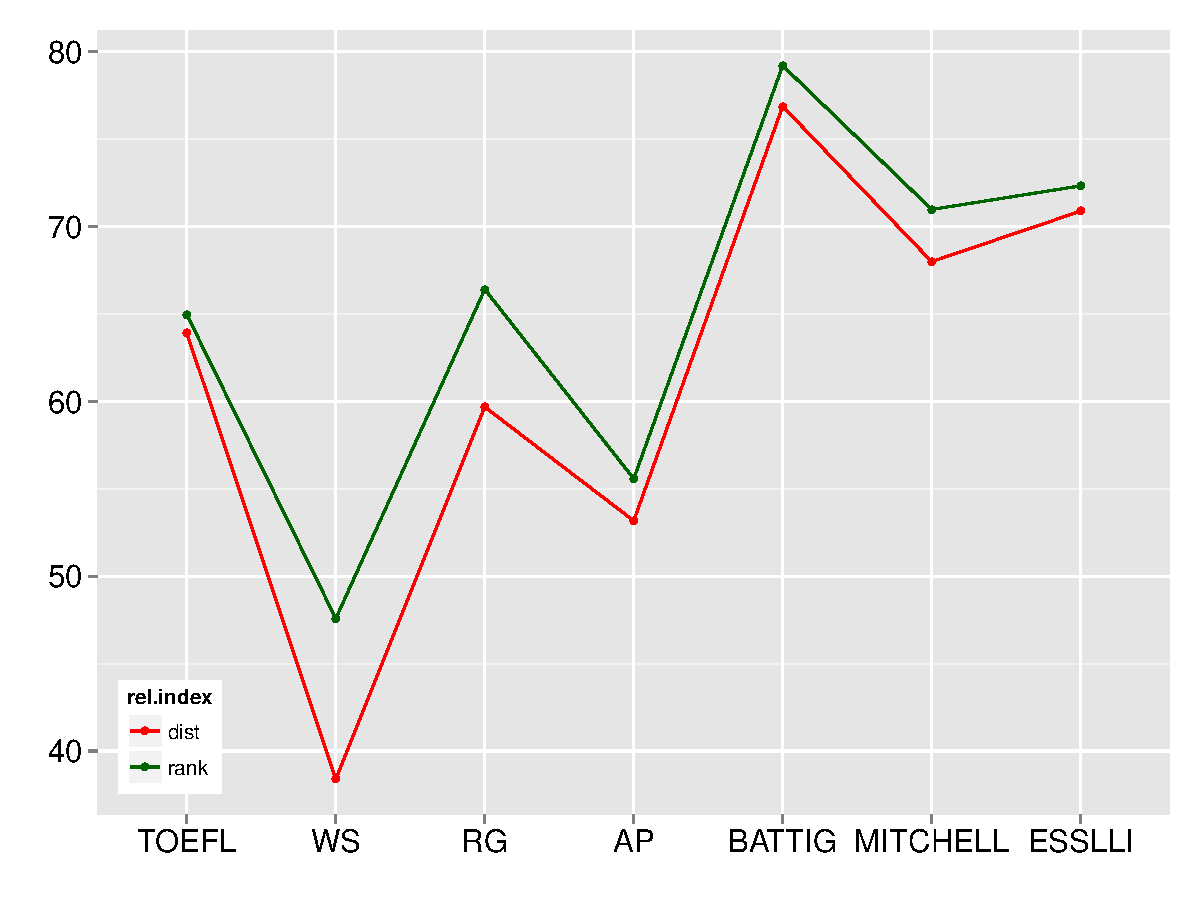
\includegraphics[scale=0.40]{img/lapesa_relindex_priming}
  \end{figure}   
  
\end{frame}

\begin{frame}
  \frametitle{Best settings and their performance}

  \begin{center}
    \setlength{\tabcolsep}{3.5pt}
    \footnotesize
    \begin{tabular}{lrlllllllllllllllll}
      \toprule
      dataset & corpus & w &  o.dim & sc & tr & m  & rel.ind & n.dim & d.sk & best.s & best.m\\ 
      \midrule
      TOEFL & ukwac & \primary{2}  & 5k & s-ll & log & cos & rank  & \primary{900} & \primary{100} & 92.5 & 98.75 \\  
      WS & wacky & \primary{4} & 50k & s-ll  & log & cos & rank   & \primary{300} & \primary{50} &  0.67  & 0.73 \\ 
      RG &  wacky & \primary{4} & 50k & s-ll  & log & cos & rank   & \primary{300} & \primary{50} & 0.86  & 0.89 \\  
      AP & wacky & \primary{4} & 20k & s-ll & log & cos & rank   & \primary{300} & \primary{0} & 0.69 & 0.76 \\ 
      BATTIG & wacky & \primary{8}  & 50k & s-ll & log & cos & rank   & \primary{500} & \primary{0} & 0.98  & 0.99 \\ 
      ESSLLI & wacky & \primary{2} & 20k & t-sc & log & cos & rank   & \primary{300} & \primary{0} & \textit{0.77} & \textit{0.98} \\   
      MITCHELL & wacky & \primary{4}  & 50k & s-ll & log & cos & rank  & \primary{500} & \primary{0} & 0.88 & 0.97 \\
      \bottomrule
    \end{tabular}

    \gap[1]
    \secondary{\normalsize Best settings for each dataset} 

    \gap[2]
    \raggedright
    \light{\small
      w = window size, o.dim = number of feature dimensions, sc = scoring function, tr = transformation, m = metric, d.sk = number of skipped dimensions, best.s = performance of best setting for this dataset,\\ best.m = performance of best run for this dataset
    }
  \end{center}
\end{frame}


\begin{frame}
  \frametitle{General settings}

  \ungap[1]
  \begin{center}
    \setlength{\tabcolsep}{3.5pt}
    \footnotesize
    \begin{tabular}{lrllllllllllllr}
      \toprule
      task & corpus & w &  o.dim & sc & tr. & m  & rel.ind  & n.dim  & d.sk \\  
      \midrule 
      TOEFL & ukwac & 2 &  5k & s-ll & log & cos & rank  & 900 & 100 \\   
      Rating & wacky & 4 & 50k & s-ll & log & cos & rank  & 300 & 50 \\  
      Clustering & wacky & 4 & 50k & s-ll & log  & cos & rank & 500 & 0 \\ 
      \primary{General} & \primary{wacky} & \primary{4} & \primary{50k} & \primary{s-ll} & \primary{log}  & \primary{cos} & \primary{rank} & \primary{500} & \primary{50} \\ 
      \bottomrule 
    \end{tabular}

    \gap[.5]
    \secondary{\normalsize General best settings} 
  \end{center}
  
  \pause
  \begin{center}
    \footnotesize
    \begin{tabular}{lccc>{\color{primary}}c>{\color{counterpoint}}c}
      \toprule
      Task & TOEFL &  RATINGS &   CLUSTERING &  GENERAL & SoA \\  
      \midrule 
      TOEFL & 92.5 & 85.0  & 75.0 & 90.0 & 100.0  \\  
      RG & 0.85 & 0.86  & 0.84 &  0.87 & 0.86 \\  
      WS & 0.60 & 0.67 & 0.64  & 0.68 & 0.81 \\  
      AP402 & 0.60 & 0.66 & 0.67 & 0.67 & 0.79 \\  
      BATTIG & 0.85   & 0.91 & 0.98 & 0.90 & 0.96 \\  
      ESSLLI & 0.70 & 0.77  & 0.80 & 0.77 & 0.91  \\  
      MITCHELL & 0.73 & 0.83 &  0.88 & 0.83 & 0.94 \\
      \bottomrule
    \end{tabular}

    \gap[.5]
    \secondary{\normalsize General best settings -- Performance}
  \end{center}
\end{frame}


%%%%%%%%%%%%%%%%%%%%%%%%%%%%%%%%%%%%%%%%%%%%%%%%%%%%%%%%%%%%%%%%%%%%%% 
%% References (if any)

\frame[allowframebreaks]{
\frametitle{References}
\bibliographystyle{natbib-stefan}
\begin{scriptsize}
  \bibliography{dsm}
\end{scriptsize}
}

\end{document}
